%\VignetteIndexEntry{PPBstats}
%\VignetteEngine{knitr::knitr}

\documentclass{article}\usepackage[]{graphicx}\usepackage[]{color}
%% maxwidth is the original width if it is less than linewidth
%% otherwise use linewidth (to make sure the graphics do not exceed the margin)
\makeatletter
\def\maxwidth{ %
  \ifdim\Gin@nat@width>\linewidth
    \linewidth
  \else
    \Gin@nat@width
  \fi
}
\makeatother

\definecolor{fgcolor}{rgb}{0.345, 0.345, 0.345}
\newcommand{\hlnum}[1]{\textcolor[rgb]{0.686,0.059,0.569}{#1}}%
\newcommand{\hlstr}[1]{\textcolor[rgb]{0.192,0.494,0.8}{#1}}%
\newcommand{\hlcom}[1]{\textcolor[rgb]{0.678,0.584,0.686}{\textit{#1}}}%
\newcommand{\hlopt}[1]{\textcolor[rgb]{0,0,0}{#1}}%
\newcommand{\hlstd}[1]{\textcolor[rgb]{0.345,0.345,0.345}{#1}}%
\newcommand{\hlkwa}[1]{\textcolor[rgb]{0.161,0.373,0.58}{\textbf{#1}}}%
\newcommand{\hlkwb}[1]{\textcolor[rgb]{0.69,0.353,0.396}{#1}}%
\newcommand{\hlkwc}[1]{\textcolor[rgb]{0.333,0.667,0.333}{#1}}%
\newcommand{\hlkwd}[1]{\textcolor[rgb]{0.737,0.353,0.396}{\textbf{#1}}}%
\let\hlipl\hlkwb

\usepackage{framed}
\makeatletter
\newenvironment{kframe}{%
 \def\at@end@of@kframe{}%
 \ifinner\ifhmode%
  \def\at@end@of@kframe{\end{minipage}}%
  \begin{minipage}{\columnwidth}%
 \fi\fi%
 \def\FrameCommand##1{\hskip\@totalleftmargin \hskip-\fboxsep
 \colorbox{shadecolor}{##1}\hskip-\fboxsep
     % There is no \\@totalrightmargin, so:
     \hskip-\linewidth \hskip-\@totalleftmargin \hskip\columnwidth}%
 \MakeFramed {\advance\hsize-\width
   \@totalleftmargin\z@ \linewidth\hsize
   \@setminipage}}%
 {\par\unskip\endMakeFramed%
 \at@end@of@kframe}
\makeatother

\definecolor{shadecolor}{rgb}{.97, .97, .97}
\definecolor{messagecolor}{rgb}{0, 0, 0}
\definecolor{warningcolor}{rgb}{1, 0, 1}
\definecolor{errorcolor}{rgb}{1, 0, 0}
\newenvironment{knitrout}{}{} % an empty environment to be redefined in TeX

\usepackage{alltt}

% to draw on figure or create figures
\usepackage{tikz}
\usepackage{pstricks}

\usetikzlibrary{shapes,arrows}
\graphicspath{{./figures/}}
\usepackage{wrapfig}

\usepackage{multicol}

\usepackage[utf8]{inputenc}

\usepackage[T1]{fontenc}
\usepackage[top=2cm, bottom=2cm, left=3cm, right=2cm]{geometry}
\setcounter{secnumdepth}{3}
\setcounter{tocdepth}{3}
\usepackage{url}
\usepackage[round]{natbib}
\usepackage[a4paper=true, colorlinks=true, linkcolor=black,urlcolor=blue,citecolor=black]{hyperref}


\usepackage{colortbl, xcolor}
\usepackage{float}
\usepackage{lscape}
\usepackage{multirow}

\newcommand{\pack}{\texttt{PPBstats}}
\newcommand{\R}{\texttt{R}}
\newcommand{\versionnumber}{0.13}
\newcommand{\PPB}{Participatory Plant Breeding}


% warning
\newcommand{\warning}[1]{
\setlength{\fboxrule}{1.5mm}\noindent
\begin{minipage}[t]{.1\textwidth}
\parbox[c]{\textwidth}{
\includegraphics[width=\textwidth]{warning}}
\end{minipage}
\fcolorbox{red}{white}{
\begin{minipage}[t]{.85\textwidth}
\textcolor{\colwarning}{\textbf{{#1}}}
\end{minipage}
}~\\
}
\IfFileExists{upquote.sty}{\usepackage{upquote}}{}
\begin{document}



\pagestyle{empty}
\begin{center}
\Huge{\pack } \\
\Large{An \R~package to perform analysis found within PPB programmes regarding network of seeds circulation, agronomic trials, organoleptic tests and molecular experiments}

~\\

\warning{Be aware that this package is under development and test: do not 100\% trust the functions!!! You're welcome to contribute. See for more \href{https://github.com/priviere/PPBstats/releases/download/v0.22/contribute_PPBstats.pdf}{here} details.}


~\\

version \versionnumber \\

~\\
\today

~\\~\\

Pierre Rivi\`ere\textsuperscript{1,2} \hspace{.5cm} 
Gaelle Van Frank\textsuperscript{2} \hspace{.5cm}
Olivier David\textsuperscript{3}  \hspace{.5cm} 
Facundo Muñoz\textsuperscript{4}
\\
~\\~\\ 
\end{center}

\vfill

\noindent\textsuperscript{1} R\'eseau Semences Paysannes, 3 avenue de la gare, F-47190 Aiguillon, France \\
\textsuperscript{2} INRA, UMR 0320, Génétique Quantitative et Evolution, Ferme du Moulon F-91190 Gif sur Yvette, France \\
\textsuperscript{3} INRA, UR 1404 Unité Mathématiques et Informatique Appliquées du Génome à l'Environnement, F-78352 Jouy-en-Josas, France \\ 
\textsuperscript{4} INRA, Centre Val de Loire, Unité Amélioration, Génétique et Physiologie Forestières, F-45075 Orléans, France \\ 
\textbf{Contact:} \href{mailto:pierre@semencespaysannes.org}{pierre@semencespaysannes.org} \\

\vfill

\noindent\textbf{Contributions:} \\
PR coordinates the package development, wrote the \texttt{R} functions and the vignette \\
GVF test the package and updated the code regarding Sections~\ref{ammi}, \ref{gge}, \ref{model_1}, \ref{model_2} and \ref{variance_intra} \\
OD wrote the \texttt{JAGS} code and reviewed the \texttt{R} code and the vignette regarding Sections~\ref{model_1}, \ref{model_2} and \ref{variance_intra} \\
FM reformated and improved all the code especially regarding S3 methods and reviewed and improved the vignette \\

\vfill

\begin{center}
Copyright Réseau Semences Paysannes and Institut National de la Recherche Agronomique \\
\href{http://creativecommons.org/licenses/by-nc-sa/4.0/}{Licence creative commons BY-NC-SA 4.0} \\
\vspace{.25cm}
\href{http://creativecommons.org/licenses/by-nc-sa/4.0/}{
\includegraphics[width=.15\textwidth]{cc-by-nc-sa}}
\end{center}

\clearpage

\begin{wrapfigure}{l}{.15\textwidth}
\begin{center} \vspace{-20pt}

\includegraphics[width=.15\textwidth]{Logo-RSP}
\end{center} \vspace{-20pt}
\end{wrapfigure}
\noindent
Le Réseau Semences Paysannes (the French Farmers' Seeds Network (RSP)), created in 2003, brings together a great diversity of collectives and people who preserve farmers' seeds in fields, orchards, vineyards and gardens. They are involved in supporting the consolidation of local initiatives to maintain and renew cultivated biodiversity through Community Seeds Systems. Over 80 organizations have come together to promote and develop farmers' seeds, and to protect farmers' rights over their seeds. \\
\url{www.semencespaysannes.org} (in french).


\vfill

\begin{wrapfigure}{l}{.15\textwidth}
\begin{center} \vspace{-20pt}

\includegraphics[width=.15\textwidth]{Logo-UMRGV}
\end{center} \vspace{-20pt}
\end{wrapfigure}
\noindent
The Diversity, Evolution and Adaptation of Populations (DEAP) team led by Isabelle Goldringer is part of INRA UMR 0320 Quantitative Genetic and Evolution.
Its work is based on the analysis of the genetic and evolutionary mechanisms underlying evolution and adaptation of crop populations.
DEAP develops strategies for on farm management of crop genetic diversity and
for plant breeding (evolutionary and/or participatory) adated to organic and low input agriculture.
Assessing the benefits of in-field genetic diversity (variety mixtures, populations) and designing
/ breeding optimized mixtures adapted to local conditions are also key research objectives.\\
\url{http://moulon.inra.fr/index.php/en/team/deap}


\vfill


\begin{wrapfigure}{l}{.15\textwidth}
\begin{center} \vspace{-20pt}

\includegraphics[width=.15\textwidth]{Logo-maiage}
\end{center} \vspace{-20pt}
\end{wrapfigure}
\noindent
The INRA UR1404 MaIAGE research laboratory gathers mathematicians, computer scientists, bioinformaticians and biologists to tackle problems coming from biology, agronomy and ecology; The addressed questions may concern processes at very different levels: molecular, cellular or multicellular, individual, populations, ecosystems oy landscapes. 
MaIAGE develops original methods in mathematics, statistics and computer science which are generic or driven by specific biological problems. A particular attention is paid to develop and make available softwares, databases, ontologies and web services so that biologists can use them easily to analyze their data or to mine the scientific literature.\\
\url{http://maiage.jouy.inra.fr/?q=en/home}



\newpage

\tableofcontents

\vfill

\begin{center}
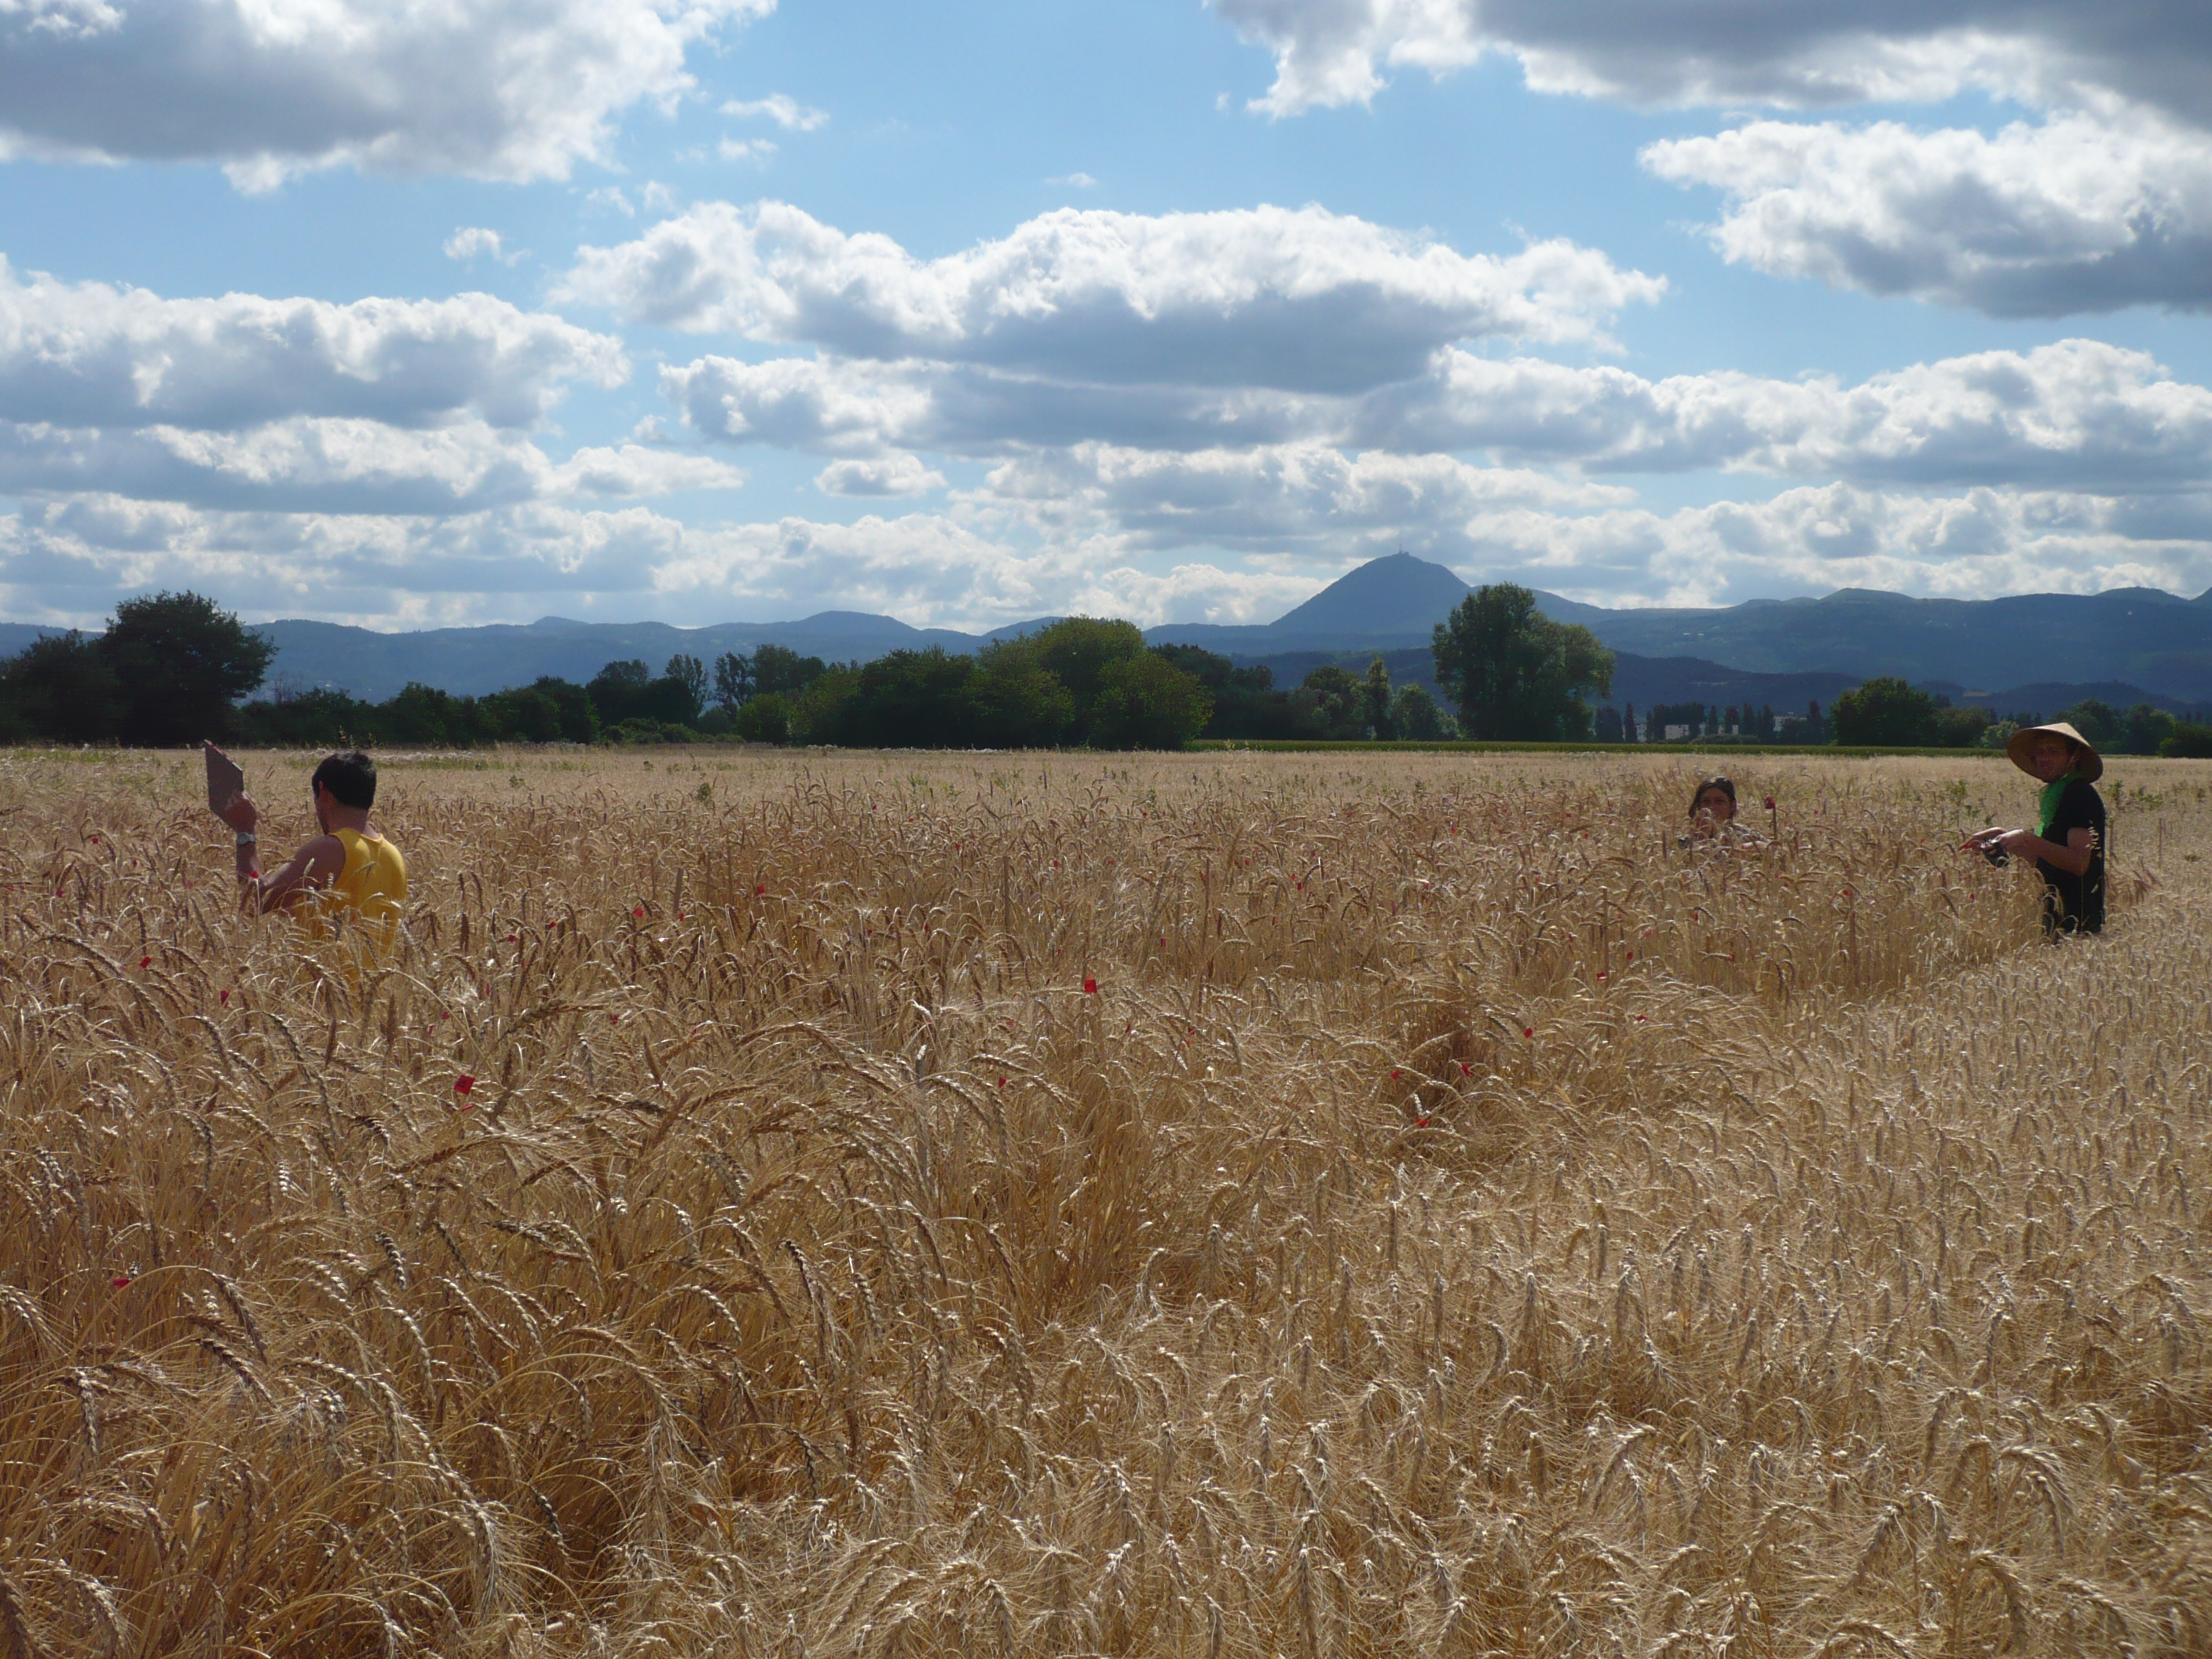
\includegraphics[width=.8\textwidth]{wheat} \\
Wheat trials on farm within our participatory plant breeding programme, summer 2012, Auvergne, France. \\
CC-BY-NC-SA. Pierre Rivière.
\end{center}

\newpage
\pagestyle{plain}



\section{Philosophy of \pack}
\label{philo}

\subsection{What is \PPB ?}

\begin{itemize}
\item \textbf{decentralized the selection}

When decentralizing the selection in target environment \citep{desclaux_changes_2008}, the phenotypic trait is the sum of genetic ($G$), environmental ($E$) and interaction between the two ($G \times E$) : $P = G + E + G \times E$.
Braod sens heritability of a given trait is then:
\begin{displaymath}
h^2_{sl} = \frac{var(G)}{var(G) + var(E) + var(G\times E)}
\end{displaymath}

Heritability taking into account the network is therefore superior or equal to heritability on a given site because $var(G\times E) > 0$.
When facing a wide diversity of agroecological environment and practices, decentralized breeding is a key point to select adapted variety to local agro-system.

\item \textbf{involve all actors in the breeding decision process}: farmers, technicians, researcher, facolitators, consumers ... Such involvement empower all actors and answer the real needs of actors  \citep{sperling_framework_2001}.

\end{itemize}


\subsection{Objectives of \pack}

\pack~aims to set, describe and analyse balanced and unbalanced trials in decentralized participatory plant breeding programmes.
The statistical procedures are based on frequentist and bayesian approaches.

\subsection{Workflow and function relations in \pack}

\pack~is divided into two sets of functions:

\begin{itemize}
\item Main functions
\item Second functions
\end{itemize}

In this vignette, we only used examples with main functions.
Nevertheless, second functions could be used in other context to answer specific questions.
Figure~\ref{main_workflow} displays the main functions and their relations.
Table~\ref{function_descriptions_workflow} describe each of the main functions.

Figure~\ref{workflow_2} display second functions used in the main functions.
Table~\ref{function_descriptions_workflow_2} describe each of the second functions.

You can have more information for each function by typing \texttt{?function\_name} in your \R~session.

%get.PPBstats.data
%extra_functions


\begin{figure}[H]
\begin{center}
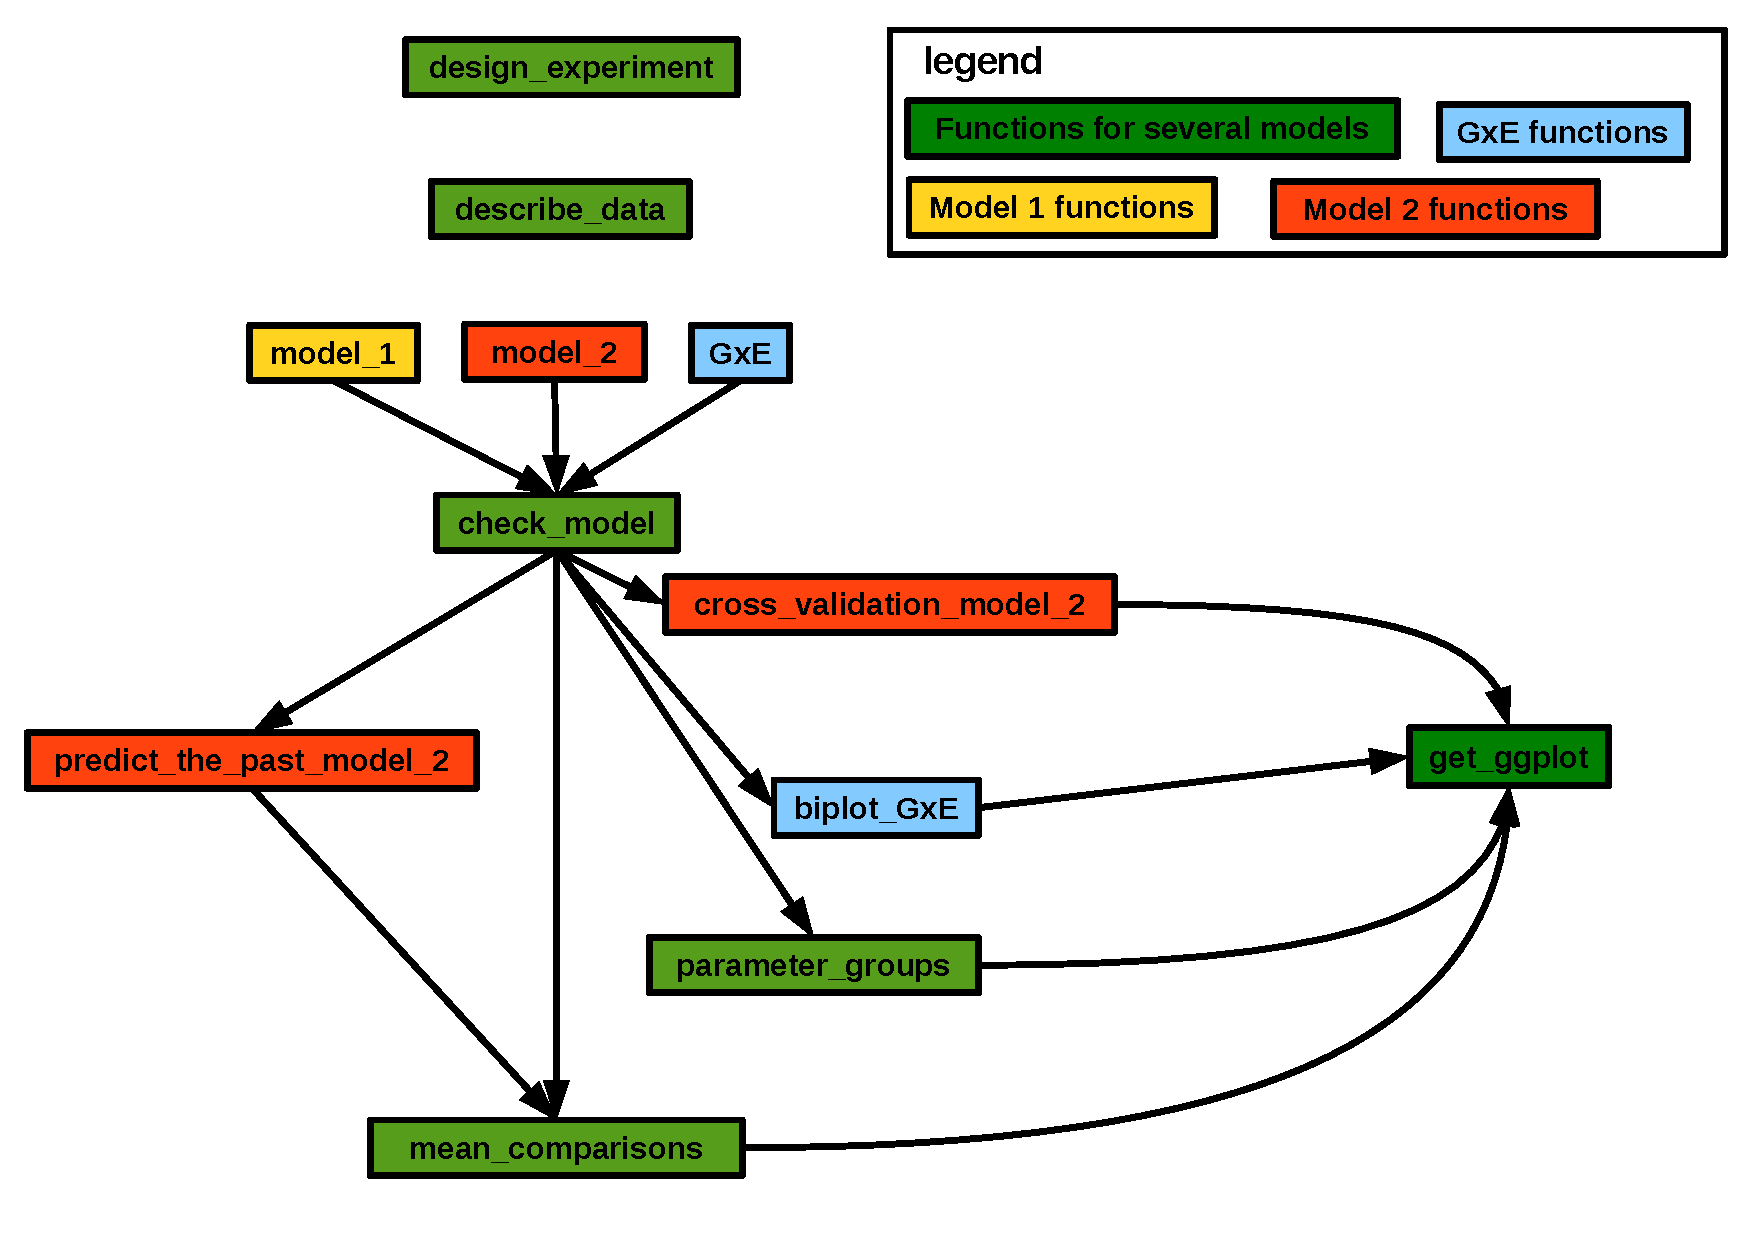
\includegraphics[width=\textwidth,page=1]{PBBstats_function_relations}
\end{center}
\caption{Main functions used in the workflow.}
\label{main_workflow}
\end{figure}

\begin{table}[H]
\begin{tabular}{cp{.6\textwidth}}

\hline
\textbf{function name} & \textbf{description} \\ \hline

\texttt{design\_experiment} & Provides experimental design for several situations \\ \hline

\texttt{describe\_data} & Describe the data set in order to choose the appropriate analysis to carry out \\ \hline

\texttt{model\_1} & Run model 1 \\ \hline

\texttt{model\_2} & Run model 2 \\ \hline

\texttt{GxE} & Run AMMI or GGE model \\ \hline

\texttt{check\_model} &  Check if the model went well \\ \hline

\texttt{mean\_comparisons} &  Get mean comparisons \\ \hline

\texttt{parameter\_groups} & Get groups of parameters based on multivariate analysis \\ \hline

\texttt{cross\_validation\_model\_2} & Run complete cross validation with model 2 \\ \hline

\texttt{predict\_the\_past\_model\_2} & Estimate value of a germplasm in an environment based on model 2 \\ \hline

\texttt{biplot\_GxE} & Compute ecovalence and format PCA results \\ \hline

\texttt{get\_ggplot} & Get ggplot objects to visualize output \\ \hline

\end{tabular}
\caption{Main function descriptions.}
\label{function_descriptions_workflow}
\end{table}


\begin{figure}[H]
\begin{center}
\includegraphics[width=\textwidth,page=2]{PBBstats_function_relations}
\includegraphics[width=\textwidth,page=3]{PBBstats_function_relations}
\end{center}
\caption{Second functions used in main functions.}
\label{workflow_2}
\end{figure}

\begin{table}[H]
\begin{tabular}{cp{.4\textwidth}}

\hline
\textbf{function name} & \textbf{description} \\ \hline

\texttt{get.env.info} & Get regional farms data and satellite farms data \\ \hline

\texttt{GxE\_build\_interaction\_matrix} & Compute interaction matrix \\ \hline

\texttt{check\_model\_model\_1} & Check if the \texttt{model\_1} model went well  \\ \hline

\texttt{check\_model\_model\_2} & Check if the \texttt{model\_2} model went well \\ \hline

\texttt{check\_model\_GxE} & Check if the GxE model went well \\ \hline

\texttt{parameter\_groups\_GxE} & Get matrix with variables in column and effect in row from \texttt{check\_model\_GxE} \\ \hline

\texttt{parameter\_groups\_model\_2} & Get matrix with variables in column and effect in row from \texttt{check\_model\_model\_2} \\ \hline

\texttt{comp.parameters} & Get parameter comparisons two by two or to a given threshold based on MCMC outputs \\ \hline

\texttt{get.significant.groups} & Get significant groups of differences for a set of parameters based on MCMC outputs \\ \hline

\texttt{get.at.least.X.groups} & Get the value of type one error needed to have X groups \\ \hline

\texttt{mean\_comparisons\_GxE} & Get mean comparisons from \texttt{check\_model\_GxE} \\ \hline

\texttt{mean\_comparisons\_model\_1} & Get mean comparisons from \texttt{check\_model\_model\_1} \\ \hline

\texttt{mean\_comparisons\_model\_2} &Get mean comparisons from \texttt{check\_model\_model\_2}  \\ \hline

\texttt{mean\_comparisons\_predict\_the\_past\_model\_2} & Get mean comparisons from \texttt{predict\_the\_past\_model\_2} \\ \hline

\texttt{ggplot\_parameter\_groups} & Get ggplot from \texttt{parameter\_groups} \\ \hline

\texttt{ggplot\_check\_model\_GxE} & Get ggplot from \texttt{check\_model\_GxE} \\ \hline

\texttt{ggplot\_check\_model\_model\_1} & Get ggplot from \texttt{check\_model\_model\_1} \\ \hline

\texttt{ggplot\_check\_model\_model\_2} & Get ggplot from \texttt{check\_model\_model\_2} \\ \hline

\texttt{ggplot\_cross\_validation\_model\_2} & Get ggplot from \texttt{cross\_validation\_model\_2} \\ \hline

\texttt{ggplot\_mean\_comparisons\_GxE} & Get ggplot from \texttt{mean\_comparisons\_GxE} \\ \hline

\texttt{ggplot\_mean\_comparisons\_model\_1} & Get ggplot from \texttt{mean\_comparisons\_model\_1} \\ \hline

\texttt{ggplot\_mean\_comparisons\_model\_2} & Get ggplot from \texttt{mean\_comparisons\_model\_2} \\ \hline

\texttt{ggplot\_mean\_comparisons\_predict\_the\_past\_model\_2} & Get ggplot from \texttt{mean\_comparisons\_predict\_the\_past\_model\_2} \\ \hline

\texttt{ggplot\_biplot\_GxE} & Get ggplot from \texttt{biplot\_GxE} \\ \hline

\texttt{ggplot\_discrimitiveness\_vs\_representativeness} & Get "discrimitiveness vs representativeness" ggplot from PCA on interaction matrix \\ \hline

\texttt{ggplot\_mean\_vs\_stability} & Get "mean vs stability" ggplot from PCA on interaction matrix \\ \hline

\texttt{ggplot\_which\_won\_where} & Get "which won where" ggplot from PCA on interaction matrix \\ \hline

\end{tabular}
\caption{Second function descriptions.}
\label{function_descriptions_workflow_2}
\end{table}

Two other funtions are also in the package:


\begin{table}[H]\begin{center}
\begin{tabular}{cl}
\hline
\texttt{common\_functions} & Some functions used in several functions of PPBstats \\ \hline
\texttt{gget.PPBstats.data} & Get PPBstats datas to run example of the vignette \\ \hline
\end{tabular}
\end{center}\end{table}



\subsection{Frequentist statistics}

!!! TO DO !!!

\subsubsection{Theory}

\subsubsection{Mean comparisons}

\subsection{Bayesian statistics}
\label{section_bayes}

\subsubsection{Theory}

The analyses performed in \pack~are based on Bayesian statistics.

Bayesian statistics are based on the Bayes theorem:

\begin{displaymath}
Pr(\theta|y) \propto Pr(\theta) Pr(y|\theta)
\end{displaymath}

with 
$Pr(\theta|y)$ the posterior, 
$Pr(y|\theta)$ the likelihood and 
$Pr(\theta)$ the prior.

The parameters' distribution, knowing the data (the posterior), is proportional to the distribution \textit{a  priori} (the prior) $\times$ the information brought by the data (the likelihood).

The more information (i.e. the larger the data set and the better the model fits the data), the less the prior would be of importance.
If the priors equal the posteriors, it means that there is not enough data or the model does not fit the data.


Bayesian inference is based on the posterior distribution of model parameters.
This distribution could not be calculated explicitely for the hierarchical model used in here (see section~\ref{section_model1} and section~\ref{section_model2}) but could be estimated using Markov Chain and Monte Carlo (MCMC) methods.

These methods simulate values of model parameters according to a Markov chain that converges to the posterior distribution of model parameters \citep{robert_bayesian_2001}.

MCMC methods were implemented using \texttt{JAGS} by the \texttt{R} package \texttt{rjags} that performed Gibbs sampling \citep{robert_bayesian_2001}.
Two MCMC chains were run independently to test for convergence using the Gelman-Rubin test.
This test was based on the variance within and between the chains \citep{gelman_inference_1992}.

A burn-in and lots of iterations were needed in the MCMC procedure.
In our case, the burn-in had 1000 iterations, then 100 000 iterations are done by default\footnote{You can change it with the argument \texttt{nb\_iterations} in functions \texttt{MC} and \texttt{FWH}} with a thinning interval of 10 to reduce autocorrelations between samples, so that 10 000 samples were available for inference for each chain by default\footnote{There are \texttt{nb\_iterations}/10 values for each chain. This can be changed with the \texttt{thin} argument of the functions.}.
 
The final distribution of a posterior is the concatenation of the two MCMC chains: 20 000 samples.


\subsubsection{Mean comparisons}
\label{mean_comp}
In this part, the mean of each entry is compared to the mean of each other entry.
Let $H_{0}$ and $H_{1}$ denote the hypotheses:

\begin{displaymath}
  H_{0} : \mu_{ij} \ge \mu_{i'j} , \; H_{1} : \mu_{ij} < \mu_{i'j}.
\end{displaymath}

The difference $\mu_{ij}-\mu_{i'j}$ between the means of germplasm $i$ and population $i'$ in environment $j$ was considered as significant if either $H_{0}$ or $H_{1}$ had a high posterior probability, that is if $Pr\{H_{0}|y\} > 1 - \alpha$ or $Pr\{H_{1}|y\}> 1 - \alpha$, where
$\alpha$ was some specified threshold.
The difference was considered as not significant otherwise.
The posterior probability of a hypothesis was estimated by the proportion of MCMC simulations for
which this hypothesis was satisfied (Figure~\ref{proba}).

Groups are made based on the probabilites.
Germplasms which share the same group are not different.
Germplasms which do not share the same groupe are different.

The threshold $\alpha$ that depends on agronomic objectives.
This threshold is set by default to $\alpha=0.1/I$ (with $I$ the number of entries in a given environnement).
It corresponded to a `soft' Bonferroni correction, the Bonferroni correction being very conservative.

As one objective of this PPB programme is that farmers (re)learn selection, the threshold could be adjusted to allow the detection of at least two groups instead of having farmers choose at random.
The initial value could be set to $\alpha=0.1/I$ and if only one group is obtained, then this value could be adjusted to allow the detection of two groups.
In this cases, the farmers should be informed of the lower degree of confidence that there are significant differences among entries.

\begin{figure}[H]
\begin{center}
\begin{pspicture}(10,10)
\rput[bl](0,0){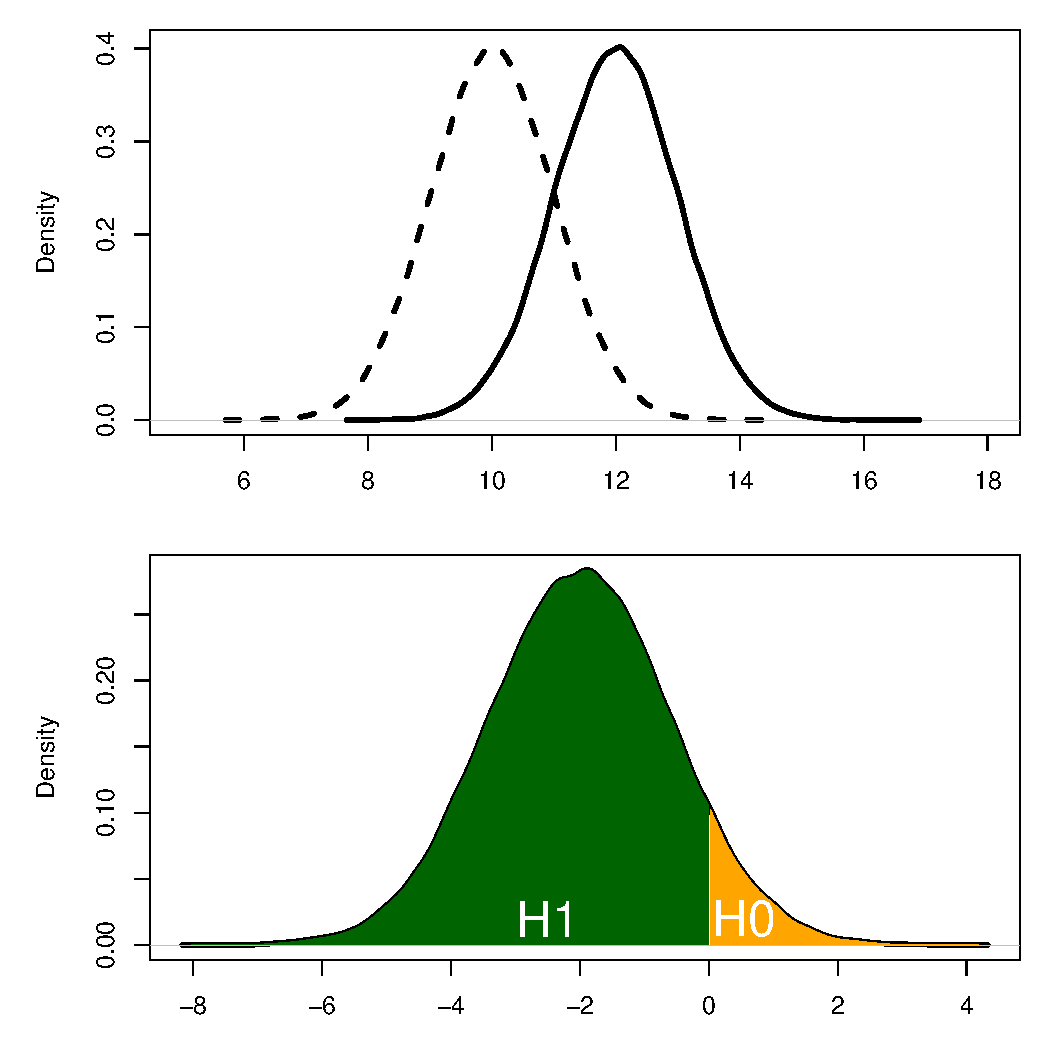
\includegraphics[width=.6\textwidth]{proba}}
\rput[b](3,7){$\mu_{ij}$}
\rput[b](7.5,7){$\mu_{i'j}$}
\rput[b](3,3){$\mu_{ij} - \mu_{i'j}$}
\end{pspicture}
\end{center}
\caption{Mean comparison between $\mu_{ij}$ (dash line) and $\mu_{i'j}$ (plain line).}
\label{proba}
\end{figure}

%% R code to get proba.pdf %%
%
%pdf("proba.pdf")
%
%par(mfrow=c(2,1),mar=c(3,5,1,1))
%
%a = rnorm(100000,10)
%d <- density(a)
%plot(d, type='l', xlab="", main="", xlim=c(5,18), lty=2, lwd=3)
%
%b = rnorm(100000,12)
%d <- density(b)
%lines(d,lty=1, lwd=3)
%
%diff = a - b
%
%d <- density(diff)
%plot(d, type='l', xlab="", main="", lty=1, lwd=3)
%
%toget = which(d$x>=0)
%H0x = d$x[toget]
%H0y = d$y[toget]
%
%toget = which(d$x<0)
%H1x = d$x[toget]
%H1y = d$y[toget]
%
%x <- H0x
%y <- H0y
%polygon( c(x,rev(x)), c(rep(0,length(x)),rev(y)), border=NA, col="orange" )
%
%x <- H1x
%y <- H1y
%polygon( c(x,rev(x)), c(rep(0,length(x)),rev(y)), border=NA, col="darkgreen" )
%
%text(-2.5,0.02,"H1", cex=2, col="white")
%text(0.55,0.02,"H0", cex=2, col="white")
%
%dev.off()

In \pack, mean comparisons are done with \texttt{mean\_comparisons}.
You can choose on which parameters to run the comparison (\texttt{parameter} argument) and the $\alpha$ type one error (\texttt{alpha} argument).
The soft Bonferonni correction is applied by default (\texttt{p.adj} argument).
More informations on this function by typing \texttt{?mean\_comparisons}.


\subsection{Let's go!}
To continue, load the development version of the package:

\begin{knitrout}
\definecolor{shadecolor}{rgb}{0.969, 0.969, 0.969}\color{fgcolor}\begin{kframe}
\begin{alltt}
\hlstd{devtools}\hlopt{::}\hlkwd{install_github}\hlstd{(}\hlstr{"priviere/PPBstats"}\hlstd{)}
\end{alltt}
\end{kframe}
\end{knitrout}

, load it 

\begin{knitrout}
\definecolor{shadecolor}{rgb}{0.969, 0.969, 0.969}\color{fgcolor}\begin{kframe}
\begin{alltt}
\hlkwd{library}\hlstd{(PPBstats)}
\end{alltt}
\end{kframe}
\end{knitrout}

and download from internet the data used in this vignette (this is useful to earn lots of time!) :

\begin{knitrout}
\definecolor{shadecolor}{rgb}{0.969, 0.969, 0.969}\color{fgcolor}\begin{kframe}
\begin{alltt}
\hlkwd{get.PPBstats.data}\hlstd{()} \hlcom{# not run}
\hlcom{# |=======================================================================| 100%}
\hlcom{# The data are downloaded in ./data_PPBstats/ }
\hlcom{# You can now load the data, for example load("./data_PPBstats/out1.Rdata").}
\end{alltt}
\end{kframe}
\end{knitrout}

The data have always the following columns : location, year, germplasm, block, X, Y as factors followed by the variables.


%The example in this vignette were performed with a computer with 4 Gb of memory and the following processor : Intel(R) Core(TM) i5-4210M CPU @ 2.60GHz.
%This gives an idea about memory and processor needed to run the analysis.

\newpage


\section{Design the experiment}
\label{doe}

Before sowing, you must plan the experiment regarding your research question, the amount of seeds available, the number of locations and the space available.

\subsection{Analysis carry out in \pack}

Based on the research question, an analysis is carried on.

Table \ref{summary_analysis} summarize the analysis possible in \pack~and their specificities.
The different effects that can be estimated are:
\begin{itemize}
\item \textbf{entry}: a combinaison of a germplasm and an location or an environment
\item \textbf{germplasm}
\item \textbf{location} 
\item \textbf{environment}: a combinaison of a location and a year
\item \textbf{interaction}: interaction between germplasm and location or germplasm and environment
\item \textbf{year}
\item \textbf{migrant-resident}: migrant refers to germplasm that was not grown on previous generation on location; resident refers to germplasm that was grown  on previous generation on location.
\item \textbf{version}: version within a germplasm, for example selected vs non-selected
\end{itemize}

\noindent The analysis are divided into four families:
\begin{itemize}
\item \textbf{Family 1} gathers analysis that estimate entry effects. This is for analysis on one farm.
\item \textbf{Family 2} gathers analysis that estimate germplasm, location and interaction effects. This is for analysis in a network of farms. Estimation of environment and year effects are in option depending of the model.
\item \textbf{Family 3} gathers one analysis which estimates effects from family 1 and 2. This is for analysis in a network of farms. Environment effect can not be estimated as location and year are separated.
\item \textbf{Family 4} gathers analysis answering specific research questions. This is for analysis on one farm or more.
\end{itemize}
Within family analysis 1 and 2, the differences are in the experimental designs which are presented in the next section.

\textbf{Family 5} refers to multivariate analysis and is mentionned in section \ref{multivariate_analysis}.

\begin{table}[H]
\begin{center}
\begin{tabular}{ccccccccccc}
\hline
Family & Name & Section &
\rotatebox{90}{entry effects} &
\rotatebox{90}{germpasm effects} &
\rotatebox{90}{location effects} &
\rotatebox{90}{environments effects} &
\rotatebox{90}{interaction effects} &
\rotatebox{90}{year effects} &
\rotatebox{90}{migrant-resident effects} & 
\rotatebox{90}{version effects}
\\
\hline
1 & Anova & \ref{classic_anova} & X & & & & & & \\
  & Spatial analysis & \ref{spatial_analysis} & X & & & & & & & \\
  & Bayesian model 1 & \ref{model_1} & X & & & & & & & \\
\hline
2 & AMMI & \ref{ammi} & & X & X & (X) & X & (X) & & \\
  & GGE & \ref{gge} & & X & X & (X) & X & (X) & & \\
  & Bayesian model 2 & \ref{model_2} & & X & X & (X) & X & & & \\
\hline
3 & Bayesian model 3 & \ref{model_3} & X & X & X & & X & X & & \\
\hline
4 & Migrant-residant & \ref{migrant_residant} & X & X & (X) & (X) & (X) & (X) & X & \\
  & Version & \ref{version} & X & (X) & (X) & (X) & (X) & (X) & & X \\
\hline
\end{tabular}
\caption{Analysis carry out in \pack. X: effects that are estimated. (X): effects that can be estimated.}
\label{summary_analysis}
\end{center}
\end{table}



\subsection{Experimental design}

The experimental design is thought in relation to the analysis.
The key elements to choose an appropriate experimental designs are:
\begin{itemize}
\item the number of locations
\item the number of years
\item the replication of entries within and between locations
\end{itemize}

\noindent Function \texttt{design\_experiment} settle experimental design based on :
\begin{itemize} 
\item the number of entries
\item the number of controls per blocks
\item the number of blocks
\item the number of columns in the design. The number of rows is computed automaticaly.
\end{itemize} 

\noindent The function returns a list with
\begin{itemize} 
\item A data frame
\item An image of the experimental design
\end{itemize} 

\noindent A description of the algorithm is describe in the help of the function: \texttt{?design\_experiment}.

\noindent Table \ref{cases_expe} summarize the different experimental design regarding analysis.

\begin{table}[H]
\begin{tabular}{
c
p{.1\textwidth}
p{.1\textwidth}
p{.4\textwidth}
p{.2\textwidth}
p{.1\textwidth}
}
\hline
case & number of locations & number of years & comments regarding entries replication & design of experiment & analysis \\
\hline
1 & 1 & 1 & All entries are replicated at least twice & \multirow{3}{.2\textwidth}{\texttt{fully-repicated}} & Anova \\
\cline{2-4}\cline{6-6}
  & 2 or more & 1 or more & Same entries are in all locations. All entries are replicated at least twice in each location & & AMMI; GGE \\
\hline
2 & 1 & 1 & Entries not replicated. Only a control is replicated in rows and columns & \texttt{row-column} & Spatial analysis \\
\hline
3 & 25 or more & 1 or more & \multirow{3}{.35\textwidth}{All locations share a control. Entries are not replicated.} & \multirow{3}{.2\textwidth}{\texttt{satellite-farm} and \texttt{regional-farm}} & \multirow{2}{.1\textwidth}{B models 1 and 2} \\
  & 12 or more & 2 or more & & & \\
  \cline{2-3} \cline{6-6}
  & 25 or more & 3 or more & & & B model 3 \\
\hline
\end{tabular}
\caption{Experimental design specification linked to dedicated analysis. Column 'design of experiments' corresponds to the argument \texttt{expe.type} in the \texttt{design\_experiment} function.}
\label{cases_expe}
\end{table}


\subsubsection{Case 1}
\begin{knitrout}
\definecolor{shadecolor}{rgb}{0.969, 0.969, 0.969}\color{fgcolor}\begin{kframe}
\begin{alltt}
\hlstd{p_fr} \hlkwb{=} \hlkwd{design_experiment}\hlstd{(}
  \hlkwc{location} \hlstd{=} \hlstr{"Location-1"}\hlstd{,}
  \hlkwc{year} \hlstd{=} \hlstr{"2016"}\hlstd{,}
  \hlkwc{expe.type} \hlstd{=} \hlstr{"fully-replicated"}\hlstd{,}
  \hlkwc{germplasm} \hlstd{=} \hlkwd{paste}\hlstd{(}\hlstr{"germ"}\hlstd{,} \hlkwd{c}\hlstd{(}\hlnum{1}\hlopt{:}\hlnum{20}\hlstd{),} \hlkwc{sep} \hlstd{=} \hlstr{":"}\hlstd{),}
  \hlkwc{nb.blocks} \hlstd{=} \hlnum{3}\hlstd{,}
  \hlkwc{nb.cols} \hlstd{=} \hlnum{4}\hlstd{)}
\end{alltt}
\end{kframe}
\end{knitrout}

By default, the data frame is under a standard format:
\begin{knitrout}
\definecolor{shadecolor}{rgb}{0.969, 0.969, 0.969}\color{fgcolor}\begin{kframe}
\begin{alltt}
\hlkwd{head}\hlstd{(p_fr}\hlopt{$}\hlstr{"fully-replicated"}\hlopt{$}\hlstd{data.frame)}
\end{alltt}
\begin{verbatim}
##     location year germplasm block X Y
## 1 Location-1 2016   germ:12     1 A 1
## 2 Location-1 2016    germ:4     1 A 2
## 3 Location-1 2016    germ:3     1 A 3
## 4 Location-1 2016   germ:13     1 A 4
## 5 Location-1 2016   germ:15     1 A 5
## 6 Location-1 2016    germ:6     1 B 1
\end{verbatim}
\end{kframe}
\end{knitrout}

You can set the format to a SHiNeMaS\footnote{Seeds History and Network Management System, see \url{http://moulon.inra.fr/index.php/en/tranverse-team/atelier-de-bioinformatique/projects/181} for more details} reproduction template file:

\begin{knitrout}
\definecolor{shadecolor}{rgb}{0.969, 0.969, 0.969}\color{fgcolor}\begin{kframe}
\begin{alltt}
\hlstd{p_fr} \hlkwb{=} \hlkwd{design_experiment}\hlstd{(}
  \hlkwc{location} \hlstd{=} \hlstr{"Location-2"}\hlstd{,}
  \hlkwc{year} \hlstd{=} \hlstr{"2016"}\hlstd{,}
  \hlkwc{expe.type} \hlstd{=} \hlstr{"fully-replicated"}\hlstd{,}
  \hlkwc{germplasm} \hlstd{=} \hlkwd{paste}\hlstd{(}\hlstr{"germ"}\hlstd{,} \hlkwd{c}\hlstd{(}\hlnum{1}\hlopt{:}\hlnum{20}\hlstd{),} \hlkwc{sep} \hlstd{=} \hlstr{":"}\hlstd{),}
  \hlkwc{nb.blocks} \hlstd{=} \hlnum{3}\hlstd{,}
  \hlkwc{nb.cols} \hlstd{=} \hlnum{4}\hlstd{,}
  \hlkwc{return.format} \hlstd{=} \hlstr{"shinemas"}\hlstd{)}
\end{alltt}
\end{kframe}
\end{knitrout}

\begin{knitrout}
\definecolor{shadecolor}{rgb}{0.969, 0.969, 0.969}\color{fgcolor}\begin{kframe}
\begin{alltt}
\hlkwd{head}\hlstd{(p_fr}\hlopt{$}\hlstr{"fully-replicated"}\hlopt{$}\hlstd{data.frame)}
\end{alltt}
\begin{verbatim}
##   project sown_year harvested_year        id_seed_lot_sown
## 1              2016                 germ:8_Location-2_2016
## 2              2016                germ:19_Location-2_2016
## 3              2016                 germ:7_Location-2_2016
## 4              2016                 germ:4_Location-2_2016
## 5              2016                germ:10_Location-2_2016
## 6              2016                 germ:3_Location-2_2016
##   intra_selection_name etiquette split quantity_sown
## 1                                                   
## 2                                                   
## 3                                                   
## 4                                                   
## 5                                                   
## 6                                                   
##   quantity_harvested block X Y
## 1                        1 A 1
## 2                        1 A 2
## 3                        1 A 3
## 4                        1 A 4
## 5                        1 A 5
## 6                        1 B 1
\end{verbatim}
\end{kframe}
\end{knitrout}


\begin{knitrout}
\definecolor{shadecolor}{rgb}{0.969, 0.969, 0.969}\color{fgcolor}\begin{kframe}
\begin{alltt}
\hlstd{p_fr}\hlopt{$}\hlstr{"fully-replicated"}\hlopt{$}\hlstd{design}
\end{alltt}
\end{kframe}

{\centering 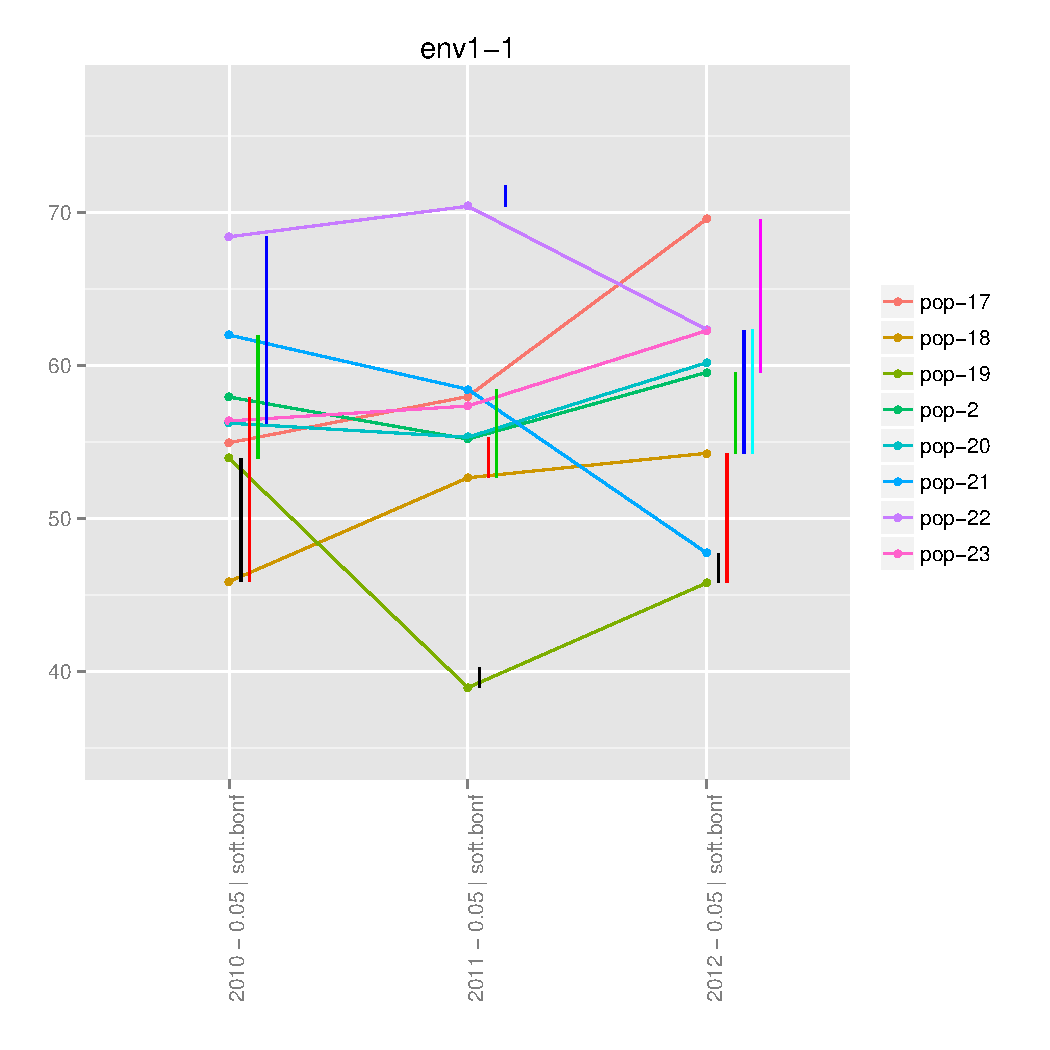
\includegraphics[width=.4\textwidth]{figures/PPBstats_unnamed-chunk-23-1} 

}



\end{knitrout}



\subsubsection{Case 2}
\begin{knitrout}
\definecolor{shadecolor}{rgb}{0.969, 0.969, 0.969}\color{fgcolor}\begin{kframe}
\begin{alltt}
\hlstd{p_case2} \hlkwb{=} \hlkwd{design_experiment}\hlstd{(}
  \hlkwc{location} \hlstd{=} \hlstr{"Location-3"}\hlstd{,}
  \hlkwc{year} \hlstd{=} \hlstr{"2016"}\hlstd{,}
  \hlkwc{expe.type} \hlstd{=} \hlstr{"row-column"}\hlstd{,}
  \hlkwc{germplasm} \hlstd{=} \hlkwd{paste}\hlstd{(}\hlstr{"germ"}\hlstd{,} \hlkwd{c}\hlstd{(}\hlnum{1}\hlopt{:}\hlnum{20}\hlstd{),} \hlkwc{sep} \hlstd{=} \hlstr{":"}\hlstd{),}
  \hlkwc{controls} \hlstd{=} \hlstr{"toto"}\hlstd{,}
  \hlkwc{nb.controls.per.block} \hlstd{=} \hlnum{7}\hlstd{,}
  \hlkwc{nb.blocks} \hlstd{=} \hlnum{1}\hlstd{,}
  \hlkwc{nb.cols} \hlstd{=} \hlnum{7}\hlstd{)}
\end{alltt}
\end{kframe}
\end{knitrout}

\begin{knitrout}
\definecolor{shadecolor}{rgb}{0.969, 0.969, 0.969}\color{fgcolor}\begin{kframe}
\begin{alltt}
\hlkwd{head}\hlstd{(p_case2}\hlopt{$}\hlstr{"row-column"}\hlopt{$}\hlstd{data.frame)}
\end{alltt}
\begin{verbatim}
##     location year germplasm block X Y
## 1 Location-3 2016    germ:9     1 A 1
## 2 Location-3 2016      toto     1 A 2
## 3 Location-3 2016    germ:6     1 A 3
## 4 Location-3 2016   germ:14     1 A 4
## 5 Location-3 2016    germ:5     1 B 1
## 6 Location-3 2016   germ:15     1 B 2
\end{verbatim}
\end{kframe}
\end{knitrout}

\begin{knitrout}
\definecolor{shadecolor}{rgb}{0.969, 0.969, 0.969}\color{fgcolor}\begin{kframe}
\begin{alltt}
\hlstd{p_case2}\hlopt{$}\hlstr{"row-column"}\hlopt{$}\hlstd{design}
\end{alltt}
\end{kframe}

{\centering 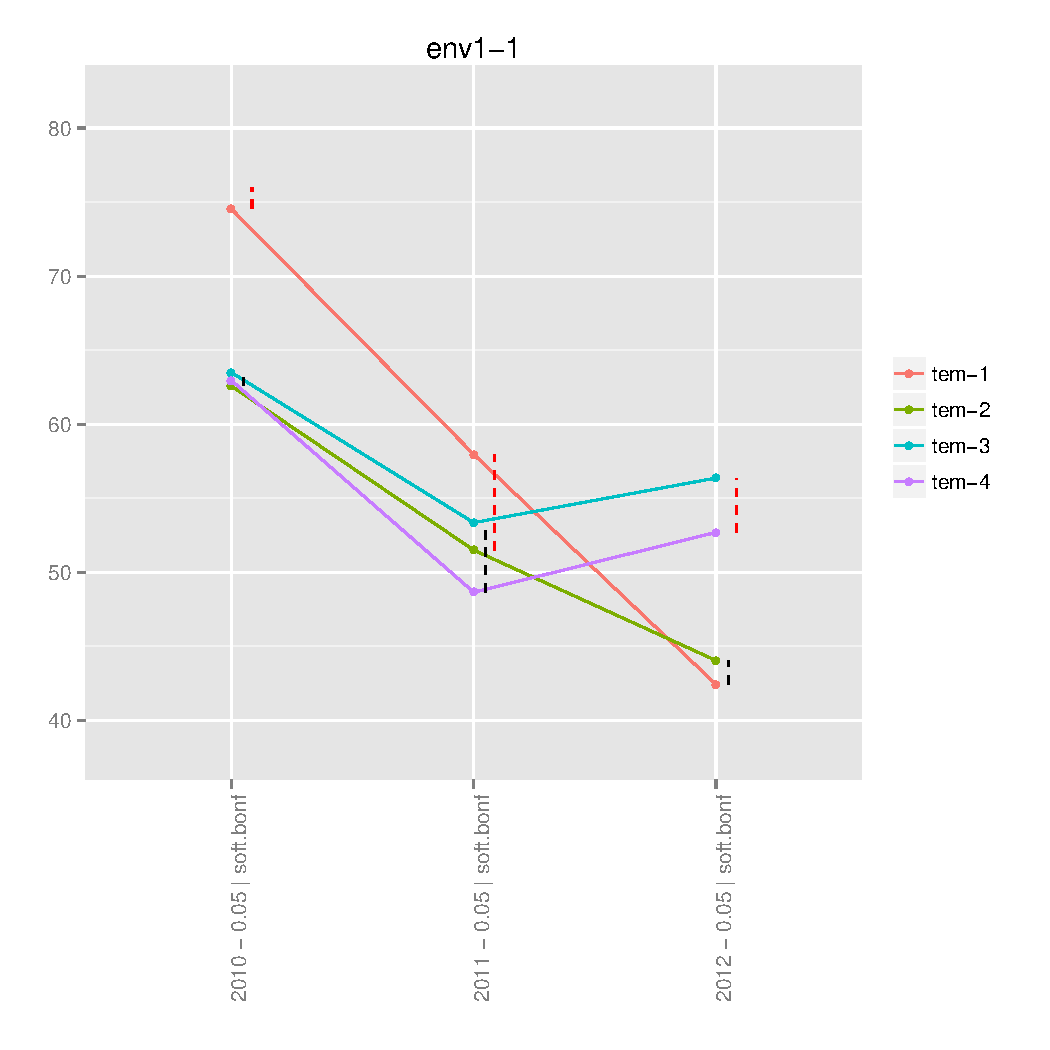
\includegraphics[width=.4\textwidth]{figures/PPBstats_unnamed-chunk-26-1} 

}



\end{knitrout}

Note that if controls are missing in rows or columns.
The function return an error.
The controls must catch as much as possible of the trial variation.


\subsubsection{Case 3}

Regional farms had several entries (i.e. a germplasm in an environment) in two or more blocks with entries replicated in each block.
Satellite farms had no block and one entry replicated twice.
Farmers chose the other entries to be sown that were not replicated.
The number of entries may vary between farms.

Here, six designs are generated: four for satellite farm and two for regional farm.

\begin{knitrout}
\definecolor{shadecolor}{rgb}{0.969, 0.969, 0.969}\color{fgcolor}\begin{kframe}
\begin{alltt}
\hlstd{p_case3_sf1} \hlkwb{=} \hlkwd{design_experiment}\hlstd{(}
  \hlkwc{location} \hlstd{=} \hlstr{"Location-4"}\hlstd{,}
  \hlkwc{year} \hlstd{=} \hlstr{"2016"}\hlstd{,}
  \hlkwc{expe.type} \hlstd{=} \hlstr{"satellite-farm"}\hlstd{,}
  \hlkwc{germplasm} \hlstd{=} \hlkwd{paste}\hlstd{(}\hlstr{"germ"}\hlstd{,} \hlkwd{c}\hlstd{(}\hlnum{1}\hlopt{:}\hlnum{6}\hlstd{),} \hlkwc{sep} \hlstd{=} \hlstr{":"}\hlstd{),}
  \hlkwc{controls} \hlstd{=} \hlstr{"toto"}\hlstd{,}
  \hlkwc{nb.controls.per.block} \hlstd{=} \hlnum{2}\hlstd{,}
  \hlkwc{nb.blocks} \hlstd{=} \hlnum{1}\hlstd{,}
  \hlkwc{nb.cols} \hlstd{=} \hlnum{2}\hlstd{)}
\hlstd{p_case3_sf1} \hlkwb{=} \hlstd{p_case3_sf1}\hlopt{$}\hlstd{`satellite-farms`}\hlopt{$}\hlstd{design}

\hlstd{p_case3_sf2} \hlkwb{=} \hlkwd{design_experiment}\hlstd{(}
  \hlkwc{location} \hlstd{=} \hlstr{"Location-5"}\hlstd{,}
  \hlkwc{year} \hlstd{=} \hlstr{"2016"}\hlstd{,}
  \hlkwc{expe.type} \hlstd{=} \hlstr{"satellite-farm"}\hlstd{,}
  \hlkwc{germplasm} \hlstd{=} \hlkwd{paste}\hlstd{(}\hlstr{"germ"}\hlstd{,} \hlkwd{c}\hlstd{(}\hlnum{1}\hlopt{:}\hlnum{6}\hlstd{),} \hlkwc{sep} \hlstd{=} \hlstr{":"}\hlstd{),}
  \hlkwc{controls} \hlstd{=} \hlstr{"toto"}\hlstd{,}
  \hlkwc{nb.controls.per.block} \hlstd{=} \hlnum{2}\hlstd{,}
  \hlkwc{nb.blocks} \hlstd{=} \hlnum{1}\hlstd{,}
  \hlkwc{nb.cols} \hlstd{=} \hlnum{2}\hlstd{)}
\hlstd{p_case3_sf2} \hlkwb{=} \hlstd{p_case3_sf2}\hlopt{$}\hlstd{`satellite-farms`}\hlopt{$}\hlstd{design}

\hlstd{p_case3_sf3} \hlkwb{=} \hlkwd{design_experiment}\hlstd{(}
  \hlkwc{location} \hlstd{=} \hlstr{"Location-6"}\hlstd{,}
  \hlkwc{year} \hlstd{=} \hlstr{"2016"}\hlstd{,}
  \hlkwc{expe.type} \hlstd{=} \hlstr{"satellite-farm"}\hlstd{,}
  \hlkwc{germplasm} \hlstd{=} \hlkwd{paste}\hlstd{(}\hlstr{"germ"}\hlstd{,} \hlkwd{c}\hlstd{(}\hlnum{1}\hlopt{:}\hlnum{6}\hlstd{),} \hlkwc{sep} \hlstd{=} \hlstr{":"}\hlstd{),}
  \hlkwc{controls} \hlstd{=} \hlstr{"toto"}\hlstd{,}
  \hlkwc{nb.controls.per.block} \hlstd{=} \hlnum{2}\hlstd{,}
  \hlkwc{nb.blocks} \hlstd{=} \hlnum{1}\hlstd{,}
  \hlkwc{nb.cols} \hlstd{=} \hlnum{2}\hlstd{)}
\hlstd{p_case3_sf3} \hlkwb{=} \hlstd{p_case3_sf3}\hlopt{$}\hlstd{`satellite-farms`}\hlopt{$}\hlstd{design}

\hlstd{p_case3_rf1} \hlkwb{=} \hlkwd{design_experiment}\hlstd{(}
  \hlkwc{location} \hlstd{=} \hlstr{"Location-7"}\hlstd{,}
  \hlkwc{year} \hlstd{=} \hlstr{"2016"}\hlstd{,}
  \hlkwc{expe.type} \hlstd{=} \hlstr{"regional-farm"}\hlstd{,}
  \hlkwc{germplasm} \hlstd{=} \hlkwd{paste}\hlstd{(}\hlstr{"germ"}\hlstd{,} \hlkwd{c}\hlstd{(}\hlnum{1}\hlopt{:}\hlnum{16}\hlstd{),} \hlkwc{sep} \hlstd{=} \hlstr{":"}\hlstd{),}
  \hlkwc{controls} \hlstd{=} \hlkwd{c}\hlstd{(}\hlstr{"c1"}\hlstd{,} \hlstr{"c2"}\hlstd{,} \hlstr{"c3"}\hlstd{,} \hlstr{"c4"}\hlstd{),}
  \hlkwc{nb.controls.per.block} \hlstd{=} \hlnum{4}\hlstd{,}
  \hlkwc{nb.blocks} \hlstd{=} \hlnum{2}\hlstd{,}
  \hlkwc{nb.cols} \hlstd{=} \hlnum{4}\hlstd{)}
\hlstd{p_case3_rf1} \hlkwb{=} \hlstd{p_case3_rf1}\hlopt{$}\hlstd{`regional-farms`}\hlopt{$}\hlstd{design}

\hlstd{p_case3_rf2} \hlkwb{=} \hlkwd{design_experiment}\hlstd{(}
  \hlkwc{location} \hlstd{=} \hlstr{"Location-8"}\hlstd{,}
  \hlkwc{year} \hlstd{=} \hlstr{"2016"}\hlstd{,}
  \hlkwc{expe.type} \hlstd{=} \hlstr{"regional-farm"}\hlstd{,}
  \hlkwc{germplasm} \hlstd{=} \hlkwd{paste}\hlstd{(}\hlstr{"germ"}\hlstd{,} \hlkwd{c}\hlstd{(}\hlnum{1}\hlopt{:}\hlnum{16}\hlstd{),} \hlkwc{sep} \hlstd{=} \hlstr{":"}\hlstd{),}
  \hlkwc{controls} \hlstd{=} \hlkwd{c}\hlstd{(}\hlstr{"c1"}\hlstd{,} \hlstr{"c2"}\hlstd{,} \hlstr{"c3"}\hlstd{),}
  \hlkwc{nb.controls.per.block} \hlstd{=} \hlnum{3}\hlstd{,}
  \hlkwc{nb.blocks} \hlstd{=} \hlnum{2}\hlstd{,}
  \hlkwc{nb.cols} \hlstd{=} \hlnum{3}\hlstd{)}
\end{alltt}


{\ttfamily\noindent\color{warningcolor}{\#\# Warning in place\_controls(d, expe.type): Controls are missing in columns 2. You can rise nb.controls.per.block.}}

{\ttfamily\noindent\color{warningcolor}{\#\# Warning in place\_controls(d, expe.type): Controls are missing in rows 2. You can rise nb.controls.per.block.}}

{\ttfamily\noindent\color{warningcolor}{\#\# Warning in place\_controls(d, expe.type): Controls are missing in columns 3. You can rise nb.controls.per.block.}}

{\ttfamily\noindent\color{warningcolor}{\#\# Warning in place\_controls(d, expe.type): Controls are missing in rows 3. You can rise nb.controls.per.block.}}\begin{alltt}
\hlstd{p_case3_rf2} \hlkwb{=} \hlstd{p_case3_rf2}\hlopt{$}\hlstd{`regional-farms`}\hlopt{$}\hlstd{design}
\end{alltt}
\end{kframe}
\end{knitrout}

If you have many space and many seeds, you can adapt the satellite farm design with only one column.
Each row beeing a sower width.

\begin{knitrout}
\definecolor{shadecolor}{rgb}{0.969, 0.969, 0.969}\color{fgcolor}\begin{kframe}
\begin{alltt}
\hlstd{p_case3_sf4} \hlkwb{=} \hlkwd{design_experiment}\hlstd{(}
  \hlkwc{location} \hlstd{=} \hlstr{"Location-9"}\hlstd{,}
  \hlkwc{year} \hlstd{=} \hlstr{"2016"}\hlstd{,}
  \hlkwc{expe.type} \hlstd{=} \hlstr{"satellite-farm"}\hlstd{,}
  \hlkwc{germplasm} \hlstd{=} \hlkwd{paste}\hlstd{(}\hlstr{"germ"}\hlstd{,} \hlkwd{c}\hlstd{(}\hlnum{1}\hlopt{:}\hlnum{6}\hlstd{),} \hlkwc{sep} \hlstd{=} \hlstr{":"}\hlstd{),}
  \hlkwc{controls} \hlstd{=} \hlstr{"C"}\hlstd{,}
  \hlkwc{nb.controls.per.block} \hlstd{=} \hlnum{2}\hlstd{,}
  \hlkwc{nb.blocks} \hlstd{=} \hlnum{1}\hlstd{,}
  \hlkwc{nb.cols} \hlstd{=} \hlnum{1}\hlstd{)}
\hlstd{p_case3_sf4} \hlkwb{=} \hlstd{p_case3_sf4}\hlopt{$}\hlstd{`satellite-farms`}\hlopt{$}\hlstd{design}
\end{alltt}
\end{kframe}
\end{knitrout}

\begin{center}
\begin{tabular}{cc}
\texttt{p\_case3\_sf1} & \texttt{p\_case3\_sf2} \\
\begin{knitrout}
\definecolor{shadecolor}{rgb}{0.969, 0.969, 0.969}\color{fgcolor}

{\centering \includegraphics[width=.4\textwidth]{figures/PPBstats_unnamed-chunk-29-1} 

}



\end{knitrout}
&
\begin{knitrout}
\definecolor{shadecolor}{rgb}{0.969, 0.969, 0.969}\color{fgcolor}

{\centering 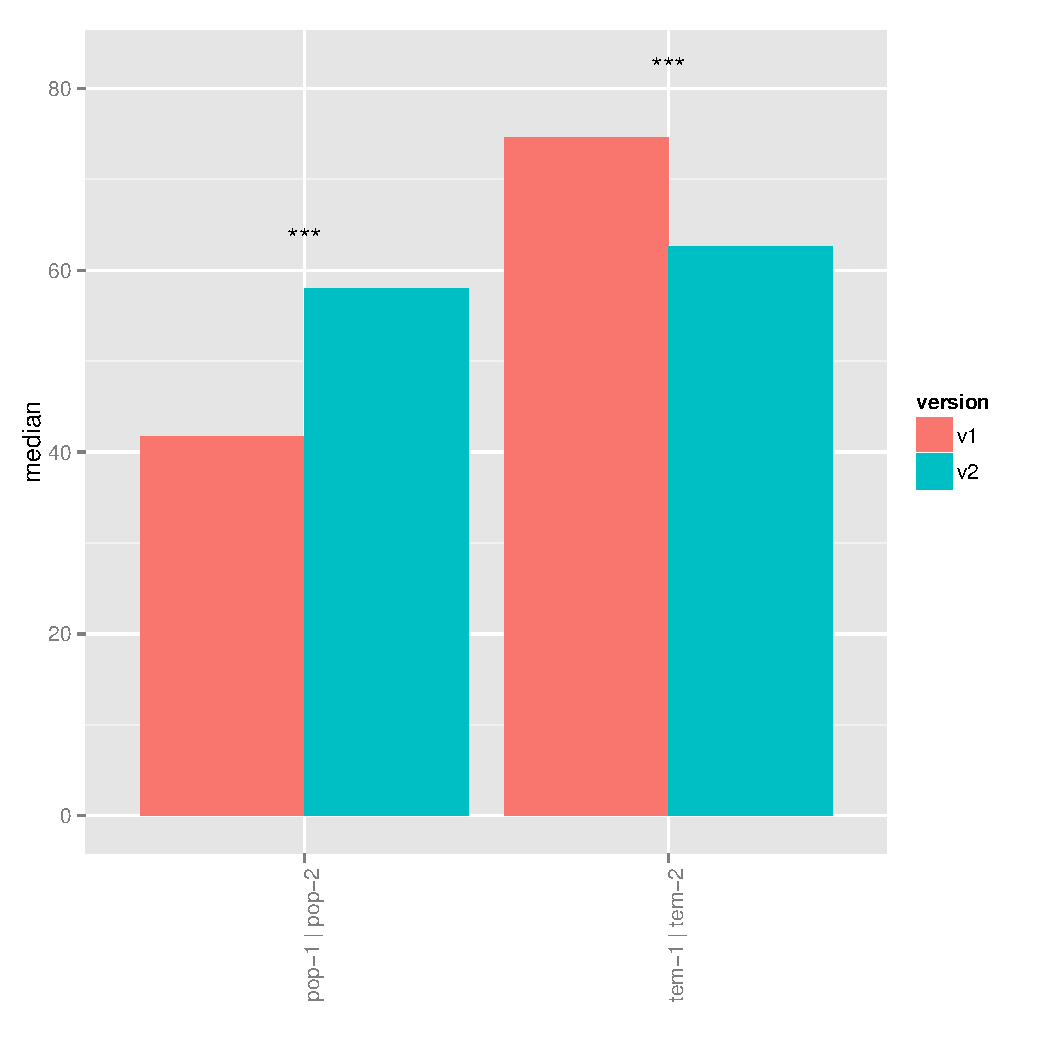
\includegraphics[width=.4\textwidth]{figures/PPBstats_unnamed-chunk-30-1} 

}



\end{knitrout}
\\
\texttt{p\_case3\_sf3} & \texttt{p\_case3\_rf1} \\
\begin{knitrout}
\definecolor{shadecolor}{rgb}{0.969, 0.969, 0.969}\color{fgcolor}

{\centering 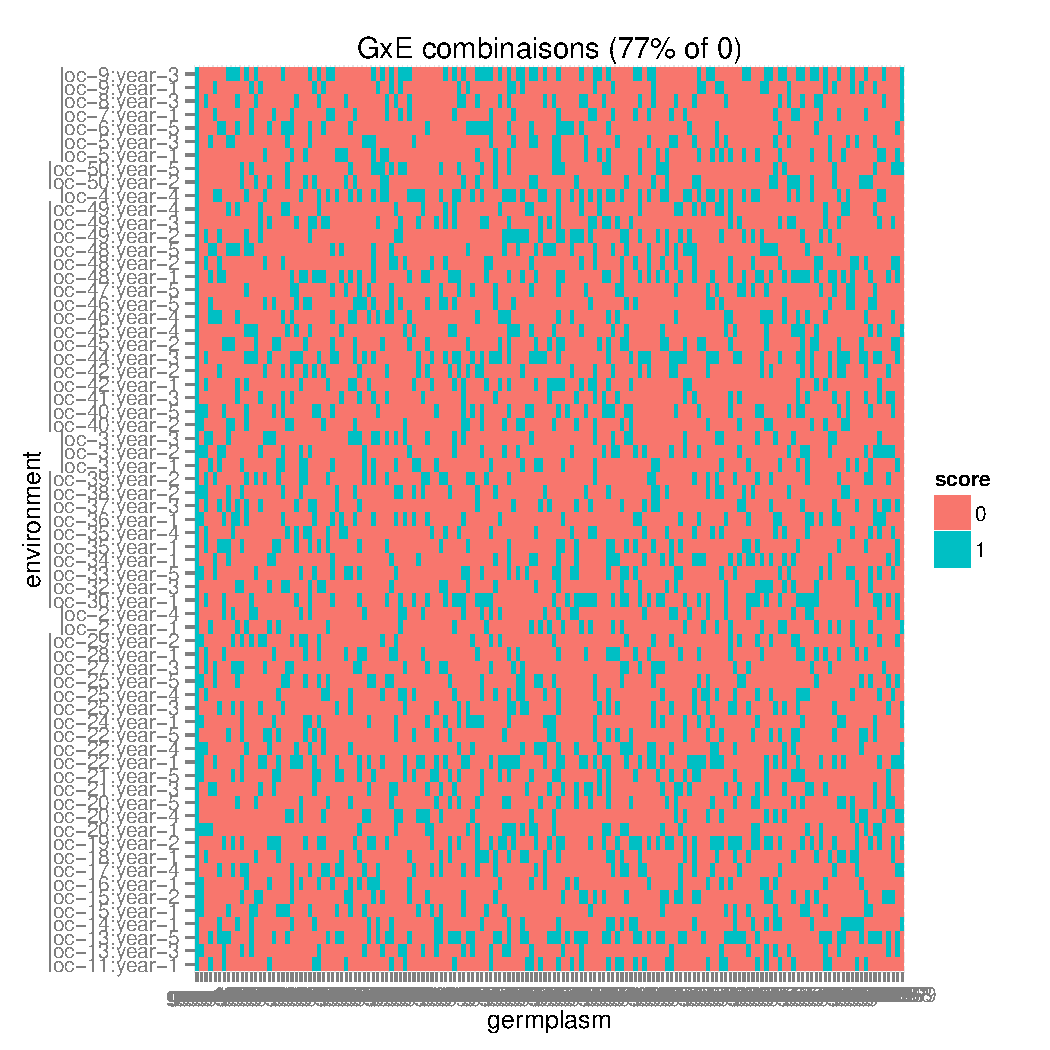
\includegraphics[width=.4\textwidth]{figures/PPBstats_unnamed-chunk-31-1} 

}



\end{knitrout}
&
\begin{knitrout}
\definecolor{shadecolor}{rgb}{0.969, 0.969, 0.969}\color{fgcolor}

{\centering 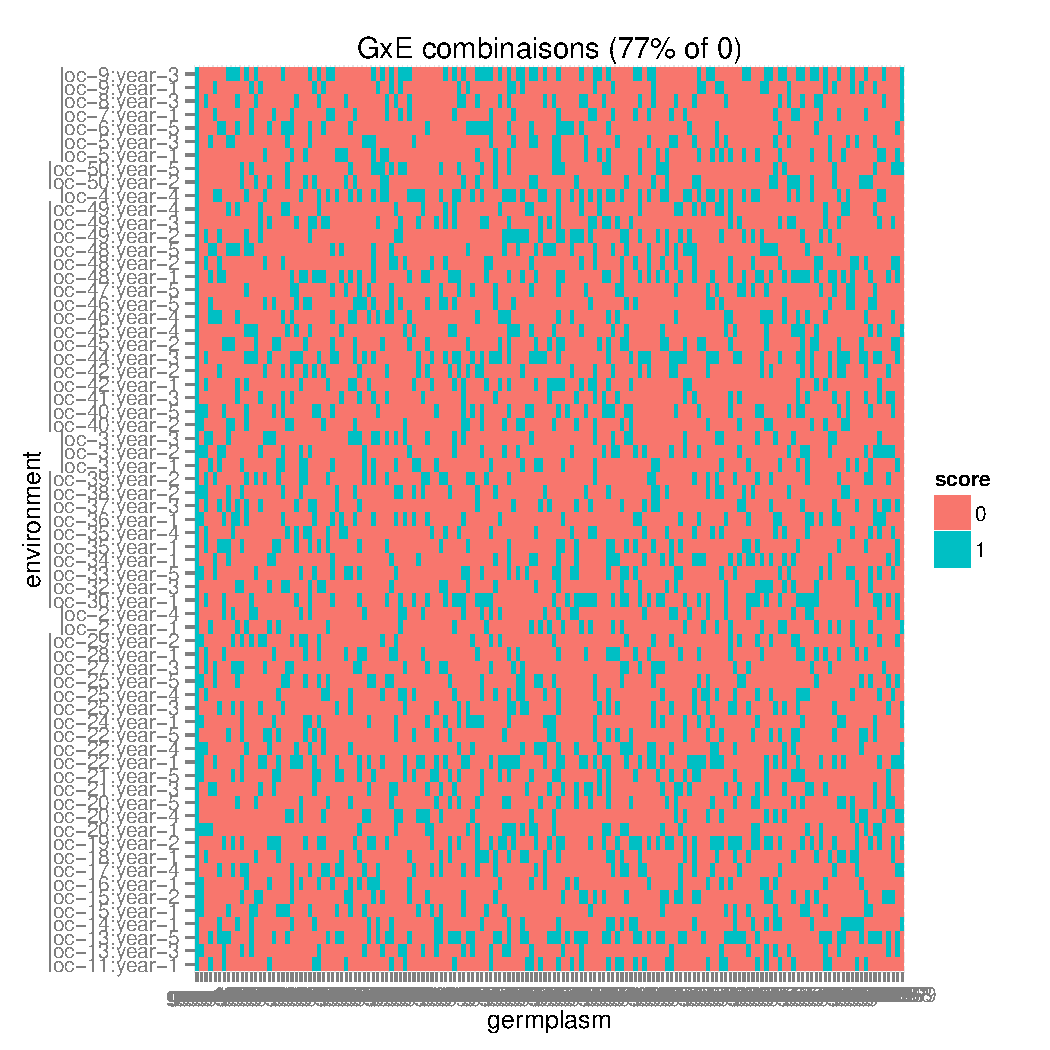
\includegraphics[width=.4\textwidth]{figures/PPBstats_unnamed-chunk-32-1} 

}



\end{knitrout}
\\
\texttt{p\_case3\_sf4} & \texttt{p\_case3\_rf2} \\
\begin{knitrout}
\definecolor{shadecolor}{rgb}{0.969, 0.969, 0.969}\color{fgcolor}

{\centering 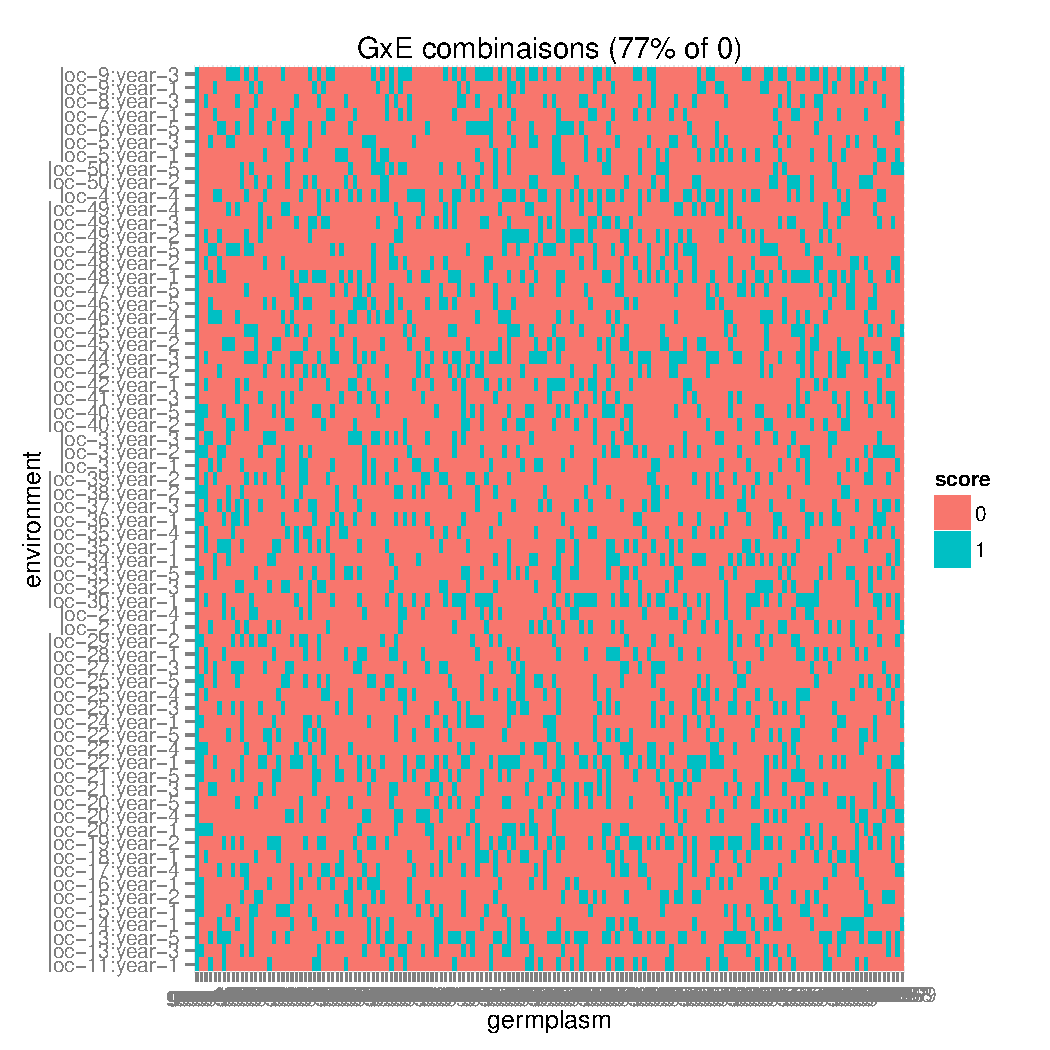
\includegraphics[width=.4\textwidth]{figures/PPBstats_unnamed-chunk-33-1} 

}



\end{knitrout}
&
\begin{knitrout}
\definecolor{shadecolor}{rgb}{0.969, 0.969, 0.969}\color{fgcolor}

{\centering 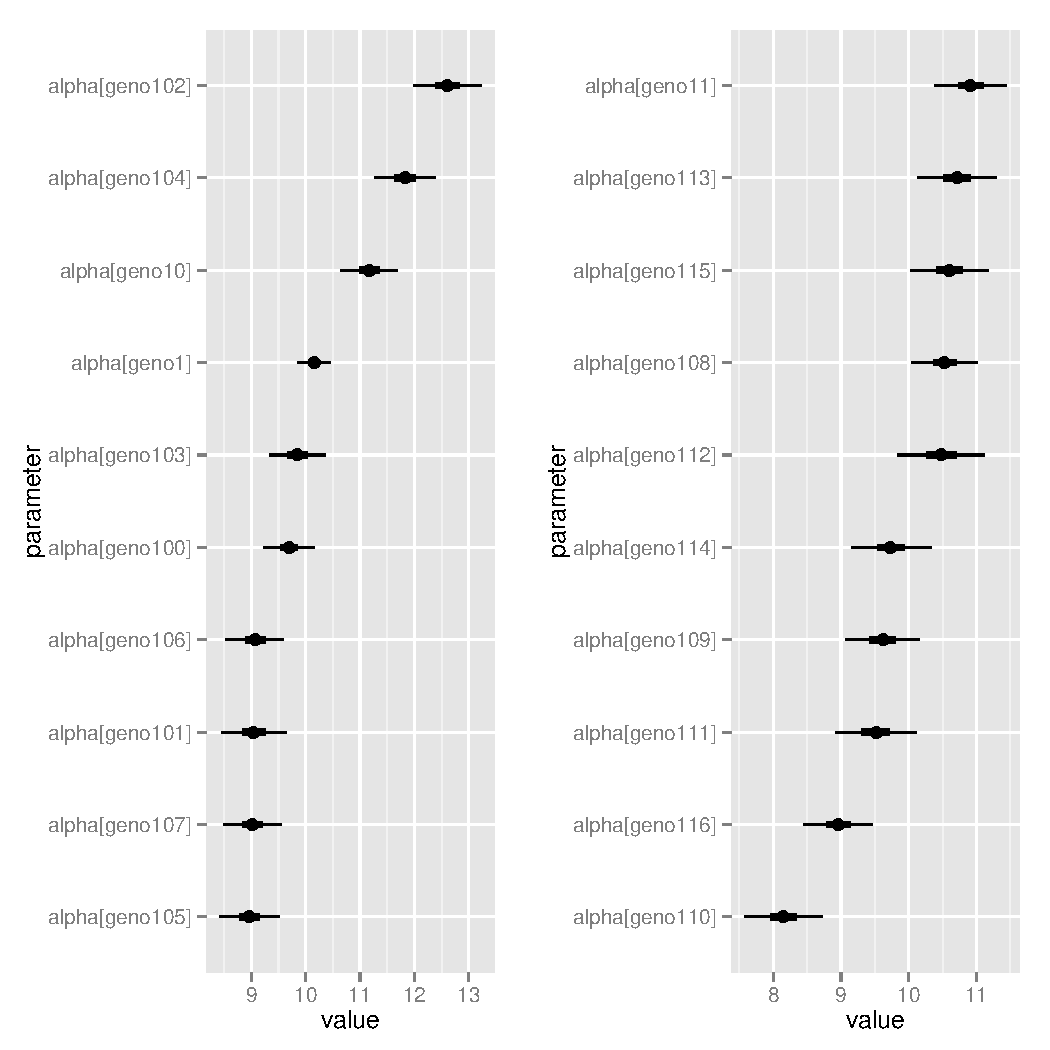
\includegraphics[width=.4\textwidth]{figures/PPBstats_unnamed-chunk-34-1} 

}



\end{knitrout}
\\
\end{tabular}
\end{center}

There some constraints regarding \texttt{expe.type = "satellite-farm"}:
\begin{itemize}
\item if \texttt{nb.entries > 10}, a warning message recommand to have less than 10 entries.
\item There are two controls per block
\item There is one block
\item There are maximum two columns
\end{itemize}

For \texttt{expe.type = "regional-farm"}, there is a warning message if controls are missing in rows or columns.
It is better to catch as much as possible of the trial variation.
If there are less than 2 blocks, an error is returned.

\subsubsection{Case ???}

Incomplete block design.
One or more block per farm.

\begin{knitrout}
\definecolor{shadecolor}{rgb}{0.969, 0.969, 0.969}\color{fgcolor}\begin{kframe}
\begin{alltt}
\hlstd{p_ibd} \hlkwb{=} \hlkwd{design_experiment}\hlstd{(}
  \hlkwc{location} \hlstd{=} \hlstr{"Location-9"}\hlstd{,}
  \hlkwc{year} \hlstd{=} \hlstr{"2016"}\hlstd{,}
  \hlkwc{expe.type} \hlstd{=} \hlstr{"IBD"}\hlstd{,}
  \hlkwc{germplasm} \hlstd{=} \hlkwd{paste}\hlstd{(}\hlstr{"germ"}\hlstd{,} \hlkwd{c}\hlstd{(}\hlnum{1}\hlopt{:}\hlnum{10}\hlstd{),} \hlkwc{sep} \hlstd{=} \hlstr{":"}\hlstd{),}
  \hlkwc{nb.blocks} \hlstd{=} \hlnum{8}\hlstd{,}
  \hlkwc{nb.cols} \hlstd{=} \hlnum{4}\hlstd{)}
\end{alltt}
\end{kframe}
\end{knitrout}

\begin{knitrout}
\definecolor{shadecolor}{rgb}{0.969, 0.969, 0.969}\color{fgcolor}\begin{kframe}
\begin{alltt}
\hlkwd{head}\hlstd{(p_ibd}\hlopt{$}\hlstd{`IBD`}\hlopt{$}\hlstd{data.frame)}
\end{alltt}
\begin{verbatim}
##   germplasm block X Y   location year
## 1    germ:1     1 A 1 Location-9 2016
## 2    germ:3     2 A 2 Location-9 2016
## 3    germ:4     3 A 3 Location-9 2016
## 4    germ:1     4 A 4 Location-9 2016
## 5    germ:2     5 A 5 Location-9 2016
## 6    germ:2     6 A 6 Location-9 2016
\end{verbatim}
\end{kframe}
\end{knitrout}


\begin{knitrout}
\definecolor{shadecolor}{rgb}{0.969, 0.969, 0.969}\color{fgcolor}\begin{kframe}
\begin{alltt}
\hlstd{p_ibd}\hlopt{$}\hlstd{`IBD`}\hlopt{$}\hlstd{design}
\end{alltt}
\end{kframe}

{\centering 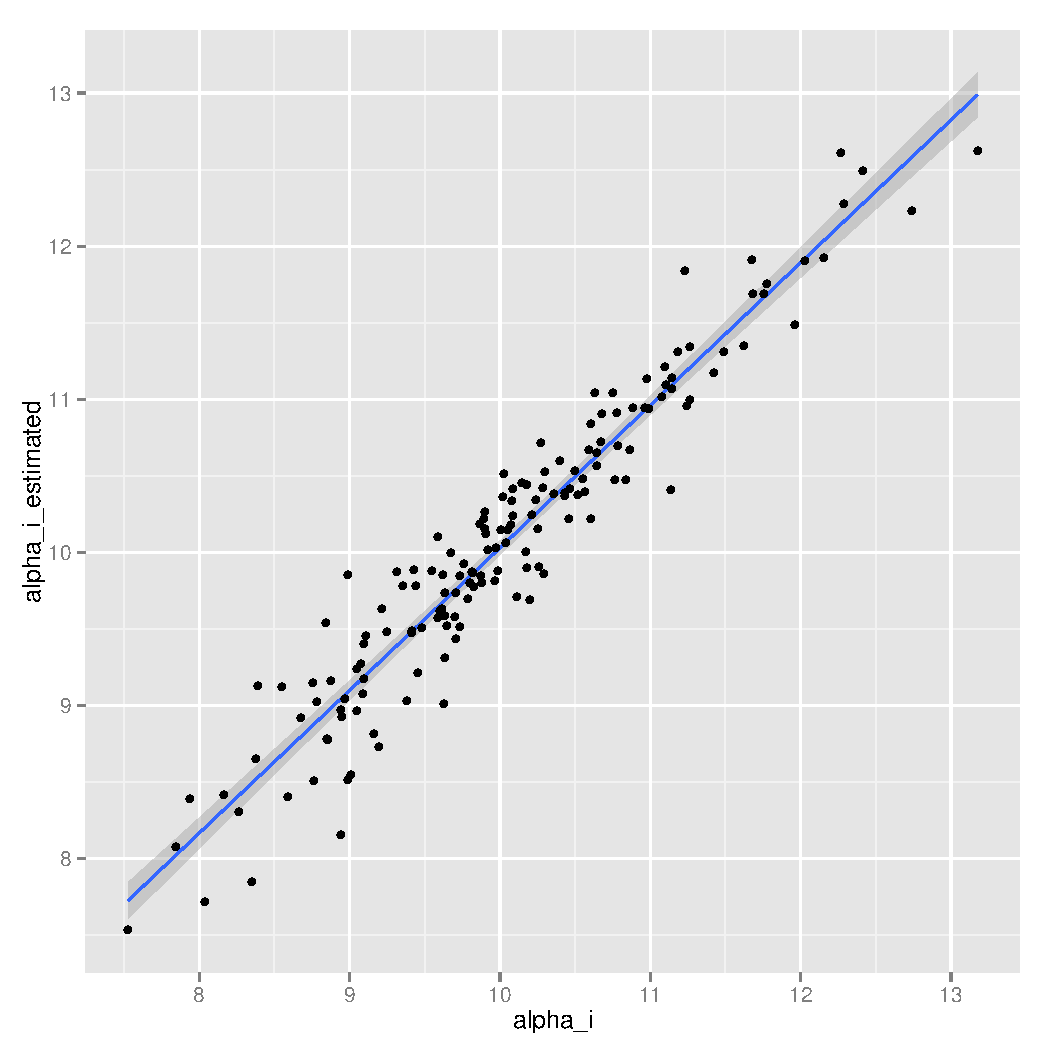
\includegraphics[width=.4\textwidth]{figures/PPBstats_unnamed-chunk-37-1} 

}



\end{knitrout}


\newpage

\section{Sow, note, harvest, measure ... }
\label{section_sow}

!!! TO DO !!!

\newpage


\section{Describe the data}
\label{describe_data}

When the data are collected, a first step is to describe it with \texttt{describe\_data}.

\begin{knitrout}
\definecolor{shadecolor}{rgb}{0.969, 0.969, 0.969}\color{fgcolor}\begin{kframe}
\begin{alltt}
\hlstd{describe_data_GxE} \hlkwb{=} \hlkwd{describe_data}\hlstd{(data_GxE,} \hlkwc{vec_variables} \hlstd{=} \hlkwd{c}\hlstd{(}\hlstr{"y1"}\hlstd{),} \hlkwc{nb_parameters_per_plot} \hlstd{=} \hlnum{5}\hlstd{)}
\hlstd{describe_data_model_2} \hlkwb{=} \hlkwd{describe_data}\hlstd{(data_model_2,} \hlkwc{vec_variables} \hlstd{=} \hlkwd{c}\hlstd{(}\hlstr{"y1"}\hlstd{),} \hlkwc{nb_parameters_per_plot} \hlstd{=} \hlnum{5}\hlstd{)}
\end{alltt}
\end{kframe}
\end{knitrout}

The function returns a list with, 
\begin{itemize}
  \item A summary of the whole data set

  \item for each variable, a list with :

  \begin{itemize}
    \item A presence.abscence plot. Note that it may be different from experimental design planned because of NA.
    The plot represents the presence/abscence matrix of G $\times$ E combinaisons. 
\begin{knitrout}
\definecolor{shadecolor}{rgb}{0.969, 0.969, 0.969}\color{fgcolor}\begin{kframe}
\begin{alltt}
\hlstd{describe_data_GxE}\hlopt{$}\hlstd{each_variable}\hlopt{$}\hlstd{y1}\hlopt{$}\hlstd{presence.abscence}
\end{alltt}
\end{kframe}

{\centering 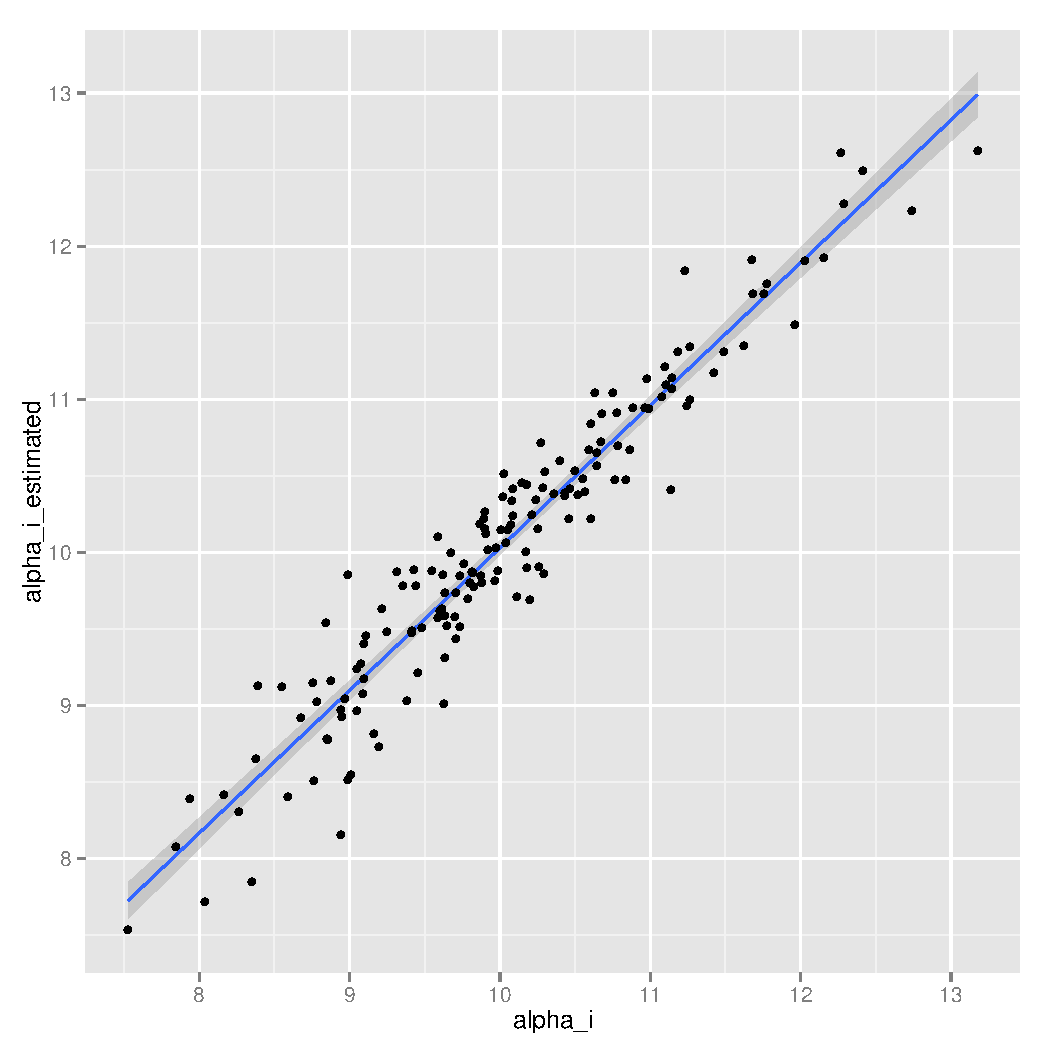
\includegraphics[width=\maxwidth]{figures/PPBstats_unnamed-chunk-39-1} 

}



\end{knitrout}
    A score of 3 is for a given germplasm replicated three times in a given environement.
    
\begin{knitrout}
\definecolor{shadecolor}{rgb}{0.969, 0.969, 0.969}\color{fgcolor}\begin{kframe}
\begin{alltt}
\hlstd{describe_data_model_2}\hlopt{$}\hlstd{each_variable}\hlopt{$}\hlstd{y1}\hlopt{$}\hlstd{presence.abscence}
\end{alltt}
\end{kframe}

{\centering 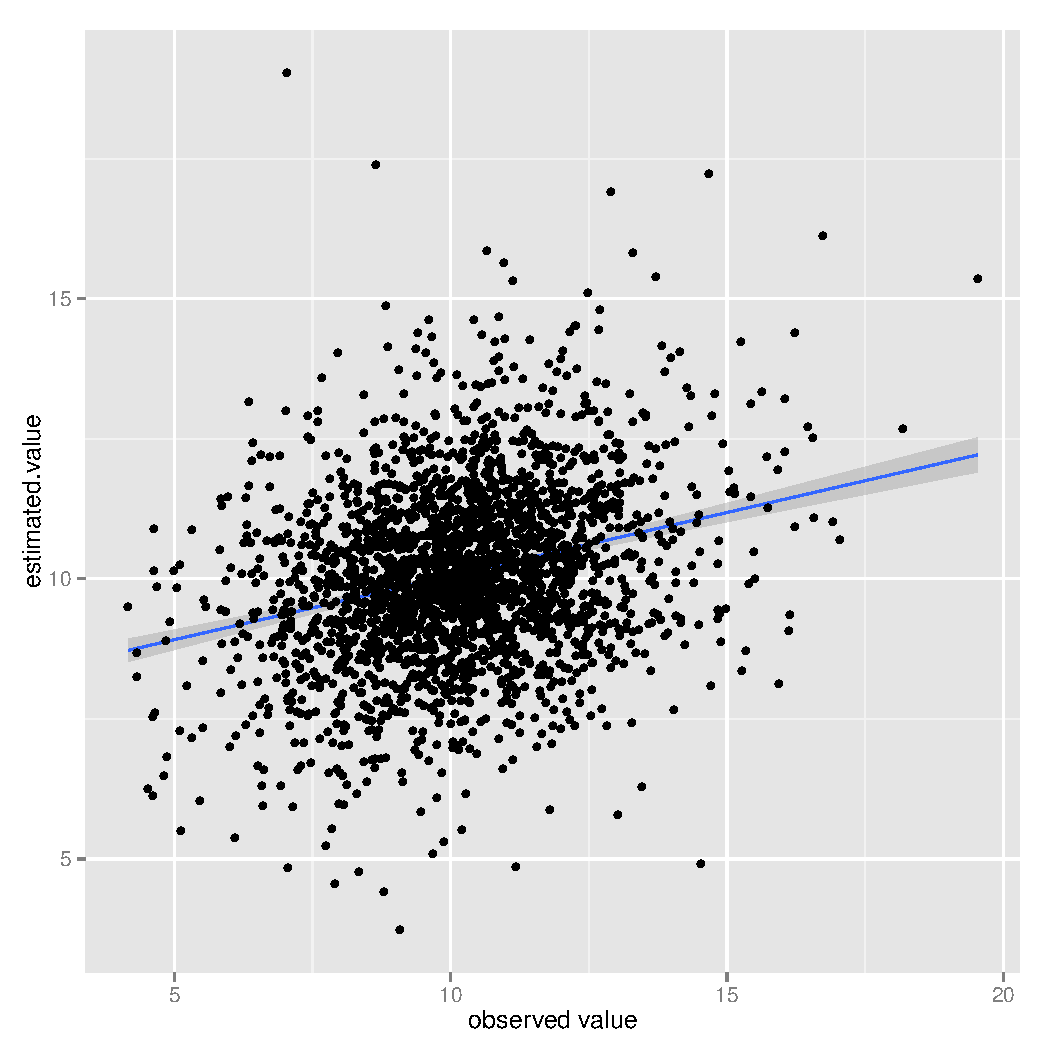
\includegraphics[width=\maxwidth]{figures/PPBstats_unnamed-chunk-40-1} 

}



\end{knitrout}
    Here there are lots of 0 meaning that a lot of germplasm are no in at least two farms.
    A score of 1 is for a given germplasm in a given environment.
    A score of 2 is for a given germplasm replicated twice in a given environement.
    
    \item A list with histogram. Note that for each element of the following list, there are as many graph as needed with \texttt{nb\_parameters\_per\_plot} parameters per graph
    \begin{itemize}
      \item germplasm
\begin{knitrout}
\definecolor{shadecolor}{rgb}{0.969, 0.969, 0.969}\color{fgcolor}\begin{kframe}
\begin{alltt}
\hlstd{pg_hist} \hlkwb{=} \hlstd{describe_data_GxE}\hlopt{$}\hlstd{each_variable}\hlopt{$}\hlstd{y1}\hlopt{$}\hlstd{histogram}\hlopt{$}\hlstd{germplasm}
\hlkwd{names}\hlstd{(pg_hist)}
\end{alltt}
\begin{verbatim}
## [1] "1" "2" "3" "4"
\end{verbatim}
\begin{alltt}
\hlstd{pg_hist}\hlopt{$}\hlstd{`1`}
\end{alltt}


{\ttfamily\noindent\itshape\color{messagecolor}{\#\# `stat\_bin()` using `bins = 30`. Pick better value with\\\#\# `binwidth`.}}\end{kframe}

{\centering 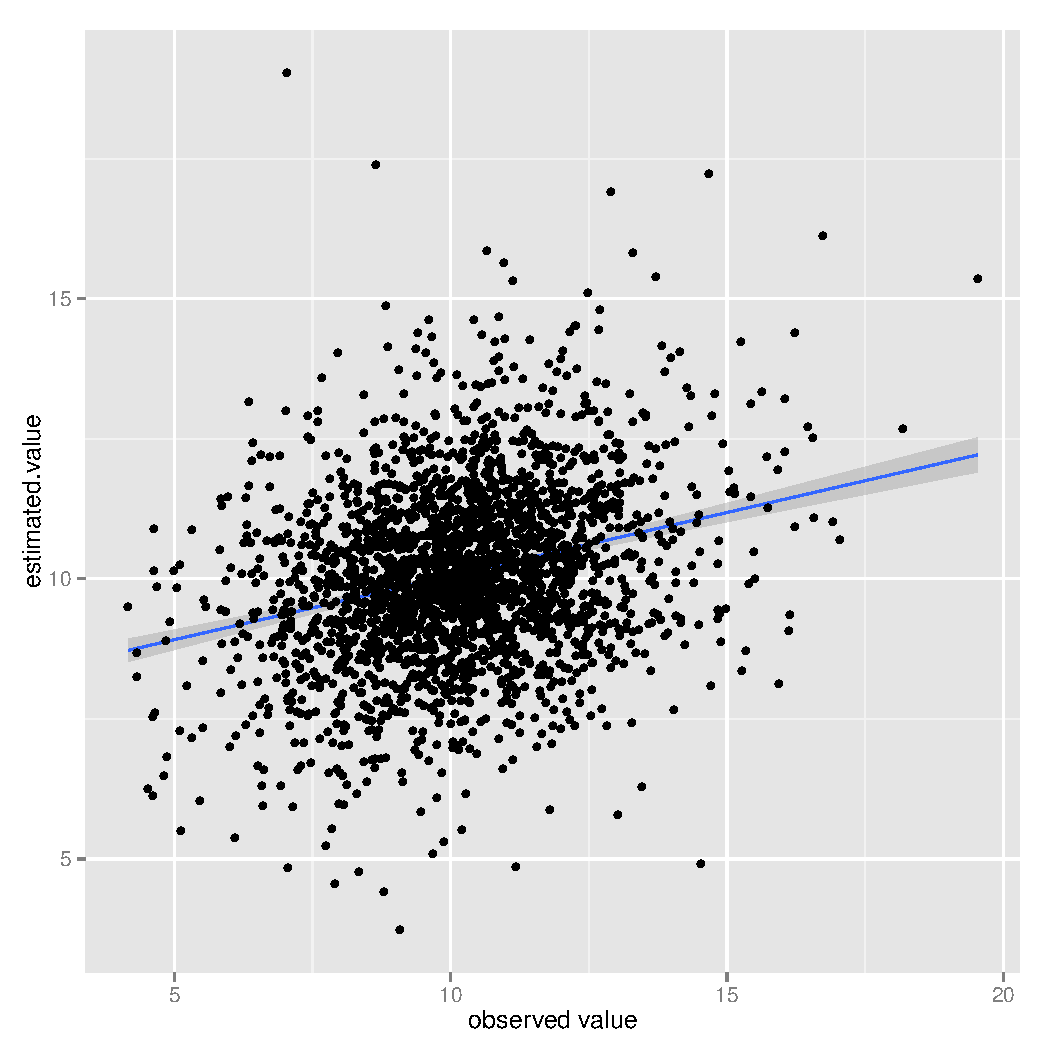
\includegraphics[width=\maxwidth]{figures/PPBstats_unnamed-chunk-41-1} 

}



\end{knitrout}
      \item location
      \item year
    \end{itemize}
    
    \item A list with boxplot, containg a list with plot and outliers. Note that for each element of the following list, there are as many graph as needed with \texttt{nb\_parameters\_per\_plot} parameters per graph
    \begin{itemize}
      \item germplasm
\begin{knitrout}
\definecolor{shadecolor}{rgb}{0.969, 0.969, 0.969}\color{fgcolor}\begin{kframe}
\begin{alltt}
\hlstd{pg_box} \hlkwb{=} \hlstd{describe_data_GxE}\hlopt{$}\hlstd{each_variable}\hlopt{$}\hlstd{y1}\hlopt{$}\hlstd{boxplot}\hlopt{$}\hlstd{germplasm}
\hlkwd{names}\hlstd{(pg_box)}
\end{alltt}
\begin{verbatim}
## [1] "1" "2" "3" "4"
\end{verbatim}
\begin{alltt}
\hlstd{pg_box}\hlopt{$}\hlstd{`1`}
\end{alltt}
\begin{verbatim}
## $plot
## 
## $outliers
## named numeric(0)
\end{verbatim}
\end{kframe}

{\centering 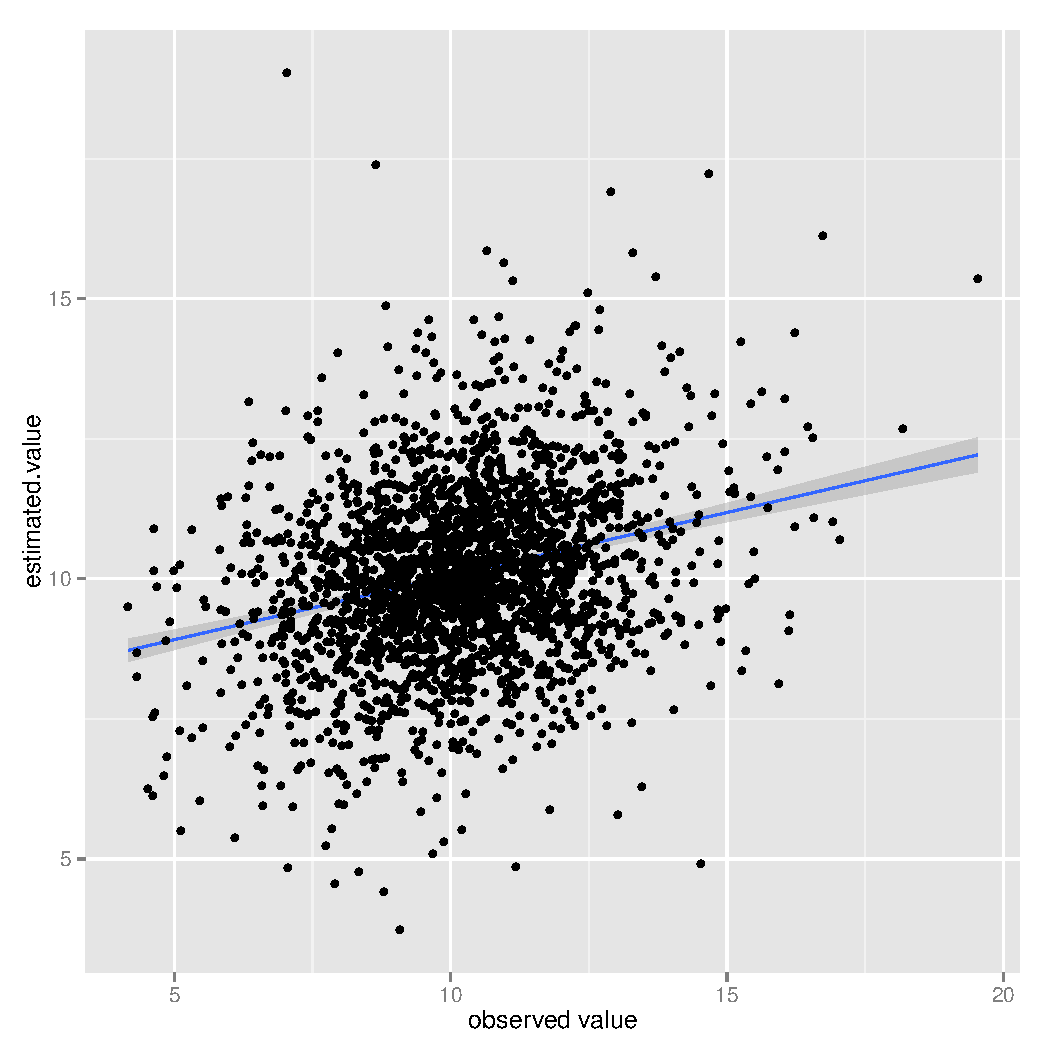
\includegraphics[width=\maxwidth]{figures/PPBstats_unnamed-chunk-42-1} 

}



\end{knitrout}
      In this example there no outliers.
      
      \item location
      \item year
    \end{itemize}
    
    \item interaction. Note that for each element of the following list, there are as many graph as needed with \texttt{nb\_parameters\_per\_plot} parameters per graph
\begin{knitrout}
\definecolor{shadecolor}{rgb}{0.969, 0.969, 0.969}\color{fgcolor}\begin{kframe}
\begin{alltt}
\hlstd{p_int} \hlkwb{=} \hlstd{describe_data_GxE}\hlopt{$}\hlstd{each_variable}\hlopt{$}\hlstd{y1}\hlopt{$}\hlstd{interaction}
\hlkwd{names}\hlstd{(p_int)}
\end{alltt}
\begin{verbatim}
## [1] "1" "2" "3" "4"
\end{verbatim}
\begin{alltt}
\hlstd{p_int}\hlopt{$}\hlstd{`1`}
\end{alltt}
\end{kframe}

{\centering 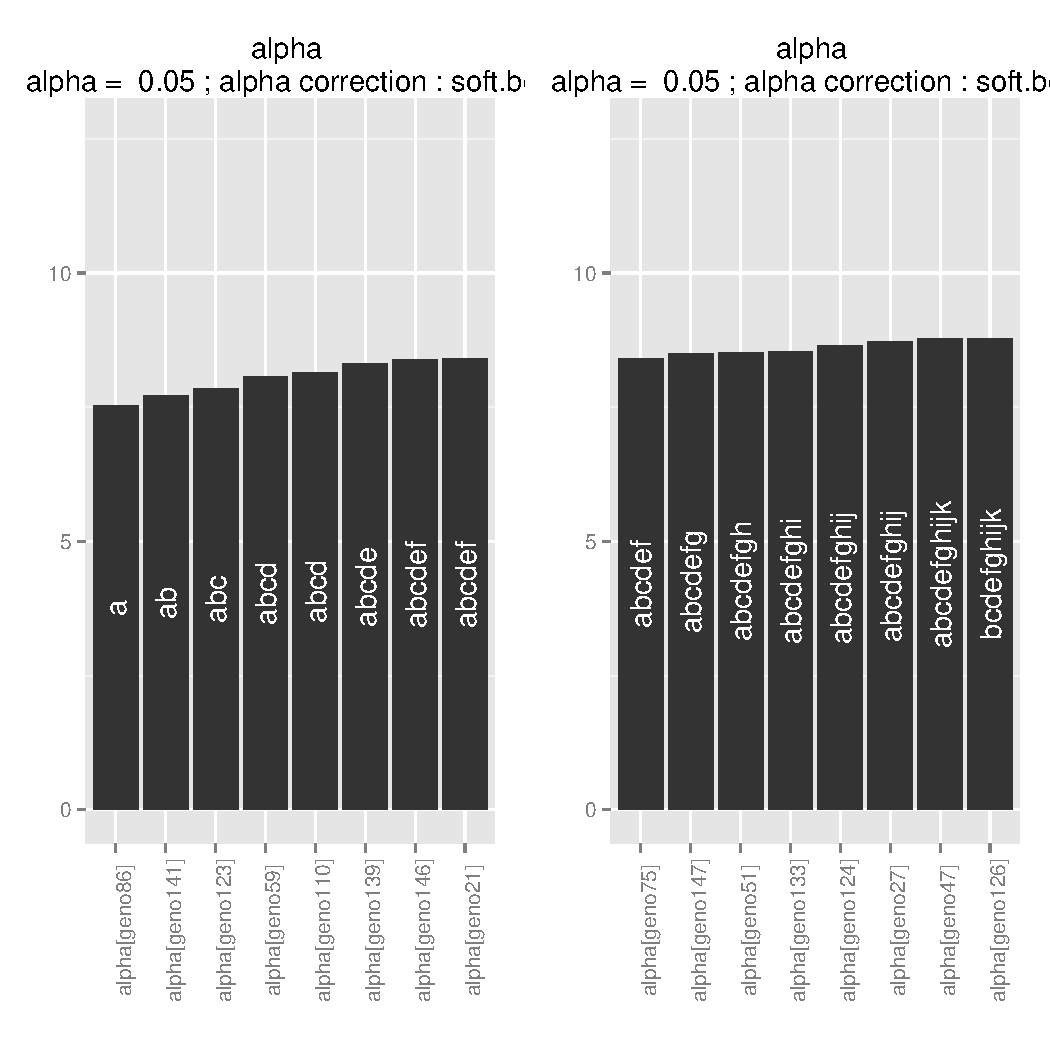
\includegraphics[width=\maxwidth]{figures/PPBstats_unnamed-chunk-43-1} 

}



\end{knitrout}
  \end{itemize}


\end{itemize}

\newpage


\section{Family of analysis 1 : entry effects on one farm}
\label{section_analysis1}


\subsection{Classic ANOVA}
\label{classic_anova}

!!! TO DO !!!

% ANOVA classique BLUEs BLUPs
\newpage


\subsection{Spatial analysis}
\label{spatial_analysis}


!!! TO DO !!!

\newpage


\subsection{model\_1 to perform mean comparisons on farms }
\label{model_1}

At the farm level, the residual had few degrees of freedom, leading to a poor estimation of the residual variance and to a lack of power for comparing populations.
Hence, model\_1 was implemented (section~\ref{section_model1}).
For model\_1, it gave nice results with more than 20 environment \citep{riviere_hierarchical_2015}.

\subsubsection{Theory of the model}

The model is describe in \citet{riviere_hierarchical_2015}.
We restricted ourselves to analysing plot means.
The phenotypic value $Y_{ijk}$ for variable $Y$, germplasm $i$, environment $j$ and block $k$ was modelled as :

\begin{equation}
	Y_{ijk} = \mu_{ij} + \beta_{jk} + \varepsilon_{ijk} ; \quad \varepsilon_{ijk} \sim \mathcal{N} (0,\sigma^2_{j}),
	\label{model1}
\end{equation}

where
$\mu_{ij}$ was the mean of germplasm $i$ in environment $j$ (note that this parameter, which corresponds to an entry, confounds the population effect and the population $\times$ environment effect);
$\beta_{jk}$ was the effect of block $k$ in environment $j$ satisfying the constraint\footnote{Note that it is quite different from \citet{riviere_hierarchical_2015} where the model was done only for two blocks. Here there is no restriction on the number of blocks.} $\sum\limits_{k=1}^K \beta_{jk} = 1$ ;
$\varepsilon_{ijk}$ was the residual error;
$\mathcal{N} (0,\sigma^2_{j})$ denoted normal distribution centred on 0 with variance $\sigma^2_{j}$, which was specific to environment $j$.

We took advantage of the similar structure of the trials on each environment of the network to assume that trial residual variances came from a common distribution :

\begin{displaymath}
	\sigma^2_{j} \sim \frac{1}{Gamma(\nu,\rho)},
\end{displaymath}

where $\nu$ and $\rho$ are unknown parameters.
Because of the low number of residual degrees of freedom for each farm, we used a hierarchical approach in order to assess mean differences on farm.
For that, we placed vague prior distributions on the hyperparameters $\nu$ and $\rho$ :

\begin{displaymath}
	\nu \sim Uniform(\nu_{min},\nu_{max}) ; \quad \rho \sim Gamma(10^{-6},10^{-6}).
\end{displaymath}


In other words, the residual variance of a trial within environment was estimated using all the informations available on the network rather than using the data from that particular trial only.

The parameters $\mu_{ij}$ and $\beta_{j1}$ were assumed to follow vague prior distributions~:

\begin{displaymath}
	\mu_{ij} \sim \mathcal{N}(\mu_{.j},10^{6}); \quad \beta_{j1} \sim \mathcal{N}(0,10^{6}).
\end{displaymath}


The inverse gamma distribution has a support bounded by 0 (consistent with the definition of a variance) and may have various shapes including asymmetric distributions.
From an agronomical point of view, the assumption that trial variances were heterogeneous was consistent with organic farming: there were as many environments as farmers leading to a high heterogeneity.
Environment was here considered in a broad sense: practices (sowing date, sowing density, tilling, etc.), pedo climatic conditions, biotic and abiotic stress, \dots \citep{desclaux_changes_2008}.
Moreover, the inverse gamma distribution had conjugate properties that facilitated MCMC convergence.
This model was therefore a good choice based on both agronomic and statistical criteria.

The residual variance estimated from the controls was assumed to be representative of the residual variance of the other entries.
Blocks were included in the model only if the trial had blocks.

\subsubsection{Steps with \pack}

For model\_1, you can follow these steps (Figure \ref{main_workflow}):

\begin{enumerate}
\item Run the model with \texttt{model\_1}
\item Check model outputs with graphs to know if you can continue the analysis with \texttt{check\_model}
\item Get mean comparisons for each factor with \texttt{mean\_comparisons} and vizualise it with \texttt{get\_ggplot}
\end{enumerate}

Let's get the data.
The values for $\mu_{ij}$, $\beta_{jk}$, $\epsilon_{ijk}$ and $\sigma_j$ are the real value taken to create the dataset.
This dataset is representative of data you can get in a PPB programme.

\begin{knitrout}
\definecolor{shadecolor}{rgb}{0.969, 0.969, 0.969}\color{fgcolor}\begin{kframe}
\begin{alltt}
\hlkwd{data}\hlstd{(data_model_1)}
\hlkwd{head}\hlstd{(data_model_1)}
\end{alltt}
\begin{verbatim}
##   location year germplasm block X Y      tkw    mu_ij beta_jk
## 1   env1-1 2010     tem-1     1 1 a 72.09900 73.37224       0
## 2   env1-1 2010     tem-2     1 2 b 61.05274 61.61823       0
## 3   env1-1 2010     tem-3     1 3 c 62.99350 64.31830       0
## 4   env1-1 2010     tem-4     1 4 d 65.10909 62.57840       0
## 5   env1-1 2010     tem-1     2 5 e 77.01361 73.37224       0
## 6   env1-1 2010     tem-2     2 6 f 64.10541 61.61823       0
##   epsilon_ijk  sigma_j
## 1  -1.2732421 1.622339
## 2  -0.5654918 1.622339
## 3  -1.3248006 1.622339
## 4   2.5306946 1.622339
## 5   3.6413666 1.622339
## 6   2.4871807 1.622339
\end{verbatim}
\end{kframe}
\end{knitrout}

\subsubsection{Run the model}

To run model~\ref{model1} on the dataset, used the function \texttt{model\_1}.
You can run it on one variable.
Here it is thousand kernel weight (tkw).

By default, \texttt{model\_1} returns posteriors for 
$\mu_{ij}$ (\texttt{return.mu = TRUE}), 
$\beta_{jk}$ (\texttt{return.beta = TRUE}), 
$\sigma_j$ (\texttt{return.sigma = TRUE}), 
$\nu$ (\texttt{return.nu = TRUE}) and 
$\rho$ (\texttt{return.rho = TRUE}).
You can also get $\epsilon_{ijk}$ value with \texttt{return.espilon = TRUE}.

By default, DIC is not displayed, you may want this value to compare to other model (\texttt{DIC = TRUE}).
DIC criterion is a generalization of the AIC criterion that can be used for hierarchical models \citep{spiegelhalter_bayesian_2002}.
The smaller the DIC value, the better the model \citep{plummer_penalized_2008}.

\begin{knitrout}
\definecolor{shadecolor}{rgb}{0.969, 0.969, 0.969}\color{fgcolor}\begin{kframe}
\begin{alltt}
\hlcom{# out_model_1 = model_1(data = data_model_1, variable = "tkw", return.epsilon = TRUE)}

\hlcom{# Compiling model graph}
\hlcom{# Resolving undeclared variables}
\hlcom{# Allocating nodes}
\hlcom{# Graph information:}
\hlcom{#   Observed stochastic nodes: 976}
\hlcom{# Unobserved stochastic nodes: 927}
\hlcom{# Total graph size: 8609}
\hlcom{# }
\hlcom{# Initializing model}
\hlcom{# }
\hlcom{# |++++++++++++++++++++++++++++++++++++++++++++++++++| 100%}
\hlcom{# |**************************************************| 100%}
\hlcom{# |**************************************************| 100%}
\hlcom{# |**************************************************| 100%}

\hlkwd{load}\hlstd{(}\hlstr{"./data_PPBstats/out_model_1.RData"}\hlstd{)} \hlcom{# To save time}
\end{alltt}
\end{kframe}
\end{knitrout}

You can get informations of the environments in the dataset :

\begin{knitrout}
\definecolor{shadecolor}{rgb}{0.969, 0.969, 0.969}\color{fgcolor}\begin{kframe}
\begin{alltt}
\hlstd{out_model_1}\hlopt{$}\hlstd{vec_env_with_no_data}
\end{alltt}
\begin{verbatim}
## NULL
\end{verbatim}
\begin{alltt}
\hlstd{out_model_1}\hlopt{$}\hlstd{vec_env_with_no_controls}
\end{alltt}
\begin{verbatim}
## [1] "env5:2010"
\end{verbatim}
\begin{alltt}
\hlstd{out_model_1}\hlopt{$}\hlstd{vec_env_with_controls}
\end{alltt}
\begin{verbatim}
##  [1] "env1-1:2010"  "env1-1:2011"  "env1-1:2012"  "env1-2:2010" 
##  [5] "env1-2:2011"  "env1-2:2012"  "env1-3:2010"  "env1-3:2011" 
##  [9] "env1-3:2012"  "env1-4:2010"  "env1-4:2011"  "env1-4:2012" 
## [13] "env1-5:2011"  "env2-10:2010" "env2-10:2011" "env2-10:2012"
## [17] "env2-11:2011" "env2-11:2012" "env2-1:2010"  "env2-1:2011" 
## [21] "env2-1:2012"  "env2-12:2011" "env2-12:2012" "env2-13:2011"
## [25] "env2-13:2012" "env2-14:2011" "env2-14:2012" "env2-15:2011"
## [29] "env2-15:2012" "env2-2:2010"  "env2-2:2011"  "env2-2:2012" 
## [33] "env2-3:2010"  "env2-3:2011"  "env2-3:2012"  "env2-4:2010" 
## [37] "env2-4:2011"  "env2-4:2012"  "env2-5:2010"  "env2-5:2011" 
## [41] "env2-5:2012"  "env2-6:2010"  "env2-6:2011"  "env2-6:2012" 
## [45] "env2-7:2010"  "env2-7:2011"  "env2-7:2012"  "env2-8:2010" 
## [49] "env2-8:2011"  "env2-8:2012"  "env2-9:2010"  "env2-9:2011" 
## [53] "env2-9:2012"  "env3-1:2011"  "env3-1:2012"  "env3-2:2011" 
## [57] "env3-2:2012"  "env3-3:2011"
\end{verbatim}
\begin{alltt}
\hlstd{out_model_1}\hlopt{$}\hlstd{vec_env_RF}
\end{alltt}
\begin{verbatim}
##  [1] "env1-1:2010" "env1-1:2011" "env1-1:2012" "env1-2:2010"
##  [5] "env1-2:2011" "env1-2:2012" "env1-3:2010" "env1-3:2011"
##  [9] "env1-3:2012" "env1-4:2010" "env1-4:2011" "env1-4:2012"
## [13] "env1-5:2011" "env3-1:2011" "env3-1:2012" "env3-2:2011"
## [17] "env3-2:2012" "env3-3:2011"
\end{verbatim}
\begin{alltt}
\hlstd{out_model_1}\hlopt{$}\hlstd{vec_env_SF}
\end{alltt}
\begin{verbatim}
##  [1] "env2-10:2010" "env2-10:2011" "env2-10:2012" "env2-11:2011"
##  [5] "env2-11:2012" "env2-1:2010"  "env2-1:2011"  "env2-1:2012" 
##  [9] "env2-12:2011" "env2-12:2012" "env2-13:2011" "env2-13:2012"
## [13] "env2-14:2011" "env2-14:2012" "env2-15:2011" "env2-15:2012"
## [17] "env2-2:2010"  "env2-2:2011"  "env2-2:2012"  "env2-3:2010" 
## [21] "env2-3:2011"  "env2-3:2012"  "env2-4:2010"  "env2-4:2011" 
## [25] "env2-4:2012"  "env2-5:2010"  "env2-5:2011"  "env2-5:2012" 
## [29] "env2-6:2010"  "env2-6:2011"  "env2-6:2012"  "env2-7:2010" 
## [33] "env2-7:2011"  "env2-7:2012"  "env2-8:2010"  "env2-8:2011" 
## [37] "env2-8:2012"  "env2-9:2010"  "env2-9:2011"  "env2-9:2012"
\end{verbatim}
\end{kframe}
\end{knitrout}

Below is an example with low \texttt{nb\_iterations}:
\begin{knitrout}
\definecolor{shadecolor}{rgb}{0.969, 0.969, 0.969}\color{fgcolor}\begin{kframe}
\begin{alltt}
\hlcom{# out_model_1_bis = model_1(data = data_model_1, variable = "tkw", nb_iteration = 5000)}

\hlcom{# Compiling model graph}
\hlcom{# Resolving undeclared variables}
\hlcom{# Allocating nodes}
\hlcom{# Graph information:}
\hlcom{#   Observed stochastic nodes: 976}
\hlcom{# Unobserved stochastic nodes: 927}
\hlcom{# Total graph size: 8609}
\hlcom{# }
\hlcom{# Initializing model}
\hlcom{# }
\hlcom{# |++++++++++++++++++++++++++++++++++++++++++++++++++| 100%}
\hlcom{# |**************************************************| 100%}
\hlcom{# |**************************************************| 100%}
\hlcom{# Warning message:}
\hlcom{#   In model_1(data = data_model_1, variable = "tkw", nb_iteration = 5000) :}
\hlcom{#   nb_iterations is below 20 000, which seems small to get convergence in the MCMC.}

\hlkwd{load}\hlstd{(}\hlstr{"./data_PPBstats/out_model_1_bis.RData"}\hlstd{)} \hlcom{# To save time}
\end{alltt}
\end{kframe}
\end{knitrout}

\subsubsection{Check and visualize model outputs}

\paragraph{Check the model}

Once the model is run, it is necessary to check if the outputs can be taken with confidence.
This step is needed before going ahead in the analysis (in fact, object used in the next functions must come from \texttt{check\_model}).

\begin{knitrout}
\definecolor{shadecolor}{rgb}{0.969, 0.969, 0.969}\color{fgcolor}\begin{kframe}
\begin{alltt}
\hlcom{# out_check_model_1 = check_model(out_model_1)}

\hlcom{# The Gelman-Rubin test is running for each parameter ...}
\hlcom{# The two MCMC for each parameter converge thanks to the Gelman-Rubin test.}

\hlkwd{load}\hlstd{(}\hlstr{"./data_PPBstats/out_check_model_1.RData"}\hlstd{)} \hlcom{# To save time}
\end{alltt}
\end{kframe}
\end{knitrout}

\texttt{out\_check\_model\_1} is a list containing:

\begin{itemize}
\item \texttt{MCMC} : a data fame resulting from the concatenation of the two MCMC for each parameter. This object can be used for further analysis. There are as many columns than parameters and as many rows than iterations/thin (the thin value is 10 by default in the models).
\begin{knitrout}
\definecolor{shadecolor}{rgb}{0.969, 0.969, 0.969}\color{fgcolor}\begin{kframe}
\begin{alltt}
\hlkwd{dim}\hlstd{(out_check_model_1}\hlopt{$}\hlstd{MCMC)}
\end{alltt}
\begin{verbatim}
## [1] 20000   945
\end{verbatim}
\end{kframe}
\end{knitrout}

\item \texttt{MCMC\_conv\_not\_ok}: a data fame resulting from the concatenation of the two MCMC for each parameter for environment where  some parameters did not converge for mu and beta

\item \texttt{data\_env\_with\_no\_controls} : data frame with environnement with no controls

\item \texttt{data\_env\_whose\_param\_did\_not\_converge} : a list with data frame with environments where some parameters did not converge for mu and beta

\item \texttt{data\_ggplot} : a list containing information for ggplot:
\begin{itemize}
\item \texttt{sigma\_j}
\item \texttt{mu\_ij}
\item \texttt{beta\_jk}
\item \texttt{sigma\_j\_2}
\item \texttt{epsilon\_ijk}
\end{itemize}

\end{itemize}

When considering \texttt{out\_model\_1\_bis}:
\begin{knitrout}
\definecolor{shadecolor}{rgb}{0.969, 0.969, 0.969}\color{fgcolor}\begin{kframe}
\begin{alltt}
\hlstd{out_check_model_1_bis} \hlkwb{=} \hlkwd{check_model}\hlstd{(out_model_1_bis)}
\end{alltt}


{\ttfamily\noindent\itshape\color{messagecolor}{\#\# The Gelman-Rubin test is running for each parameter ...}}

{\ttfamily\noindent\itshape\color{messagecolor}{\#\# The two MCMC of the following parameters do not converge thanks to the Gelman-Rubin test : nu, rho, sigma[env2-2:2010]. Therefore, they are not present in MCMC output.}}

{\ttfamily\noindent\itshape\color{messagecolor}{\#\# MCMC are updated, the following environment were deleted : env2-2:2010}}

{\ttfamily\noindent\itshape\color{messagecolor}{\#\# data\_env\_whose\_param\_did\_not\_converge contains the raw data for these environments.}}\begin{alltt}
\hlcom{# The Gelman-Rubin test is running for each parameter ...}
\hlcom{# The two MCMC of the following parameters do not converge thanks to the Gelman-Rubin test : nu, rho, sigma[env2-2:2010]. Therefore, they are not present in MCMC output.}
\hlcom{# MCMC are updated, the following environment were deleted : env2-2:2010}
\hlcom{# data_env_whose_param_did_not_converge contains the raw data for these environments.}

\hlkwd{load}\hlstd{(}\hlstr{"./data_PPBstats/out_check_model_1_bis.RData"}\hlstd{)} \hlcom{# To save time}
\end{alltt}
\end{kframe}
\end{knitrout}


\paragraph{Visualize outputs}

Once the computation is done, you can visualize the results with \texttt{get\_ggplot}
\begin{knitrout}
\definecolor{shadecolor}{rgb}{0.969, 0.969, 0.969}\color{fgcolor}\begin{kframe}
\begin{alltt}
\hlstd{p_out_check_model_1} \hlkwb{=} \hlkwd{get_ggplot}\hlstd{(out_check_model_1)}
\end{alltt}


{\ttfamily\noindent\itshape\color{messagecolor}{\#\# Distribution of sigma\_j in the inverse Gamme distribution are done.}}

{\ttfamily\noindent\itshape\color{messagecolor}{\#\# The mu\_ij posterior distributions are done.}}

{\ttfamily\noindent\itshape\color{messagecolor}{\#\# The beta\_jk posterior distributions are done.}}

{\ttfamily\noindent\itshape\color{messagecolor}{\#\# The sigma\_j posterior distributions are done.}}

{\ttfamily\noindent\itshape\color{messagecolor}{\#\# The standardised residuals distributions are done.}}\end{kframe}
\end{knitrout}

\texttt{p\_out\_check\_model\_1} is a list with:

\begin{itemize}

\item \texttt{sigma\_j\_gamma} : mean of each \texttt{sigma\_j} displayed on the Inverse Gamma distribution. The first graph represent all the \texttt{sigma\_j}, the other graph represent \texttt{nb\_parameters\_per\_plot} \texttt{sigma\_j} per graph.
\begin{knitrout}
\definecolor{shadecolor}{rgb}{0.969, 0.969, 0.969}\color{fgcolor}\begin{kframe}
\begin{alltt}
\hlstd{p_out_check_model_1}\hlopt{$}\hlstd{sigma_j_gamma[[}\hlnum{1}\hlstd{]]}
\hlstd{p_out_check_model_1}\hlopt{$}\hlstd{sigma_j_gamma[[}\hlnum{2}\hlstd{]]}
\end{alltt}
\end{kframe}

{\centering \includegraphics[width=\maxwidth]{figures/PPBstats_unnamed-chunk-52-1} 
\includegraphics[width=\maxwidth]{figures/PPBstats_unnamed-chunk-52-2} 

}



\end{knitrout}

\item \texttt{mu\_ij} : distribution of each \texttt{mu\_ij} in a list with as many elements as environment. For each element of the list, there are as many graph as needed with \texttt{nb\_parameters\_per\_plot} \texttt{mu\_ij} per graph.
\begin{knitrout}
\definecolor{shadecolor}{rgb}{0.969, 0.969, 0.969}\color{fgcolor}\begin{kframe}
\begin{alltt}
\hlkwd{names}\hlstd{(p_out_check_model_1}\hlopt{$}\hlstd{mu_ij)}
\end{alltt}
\begin{verbatim}
##  [1] "env1-1:2010"  "env1-1:2011"  "env1-1:2012"  "env1-2:2010" 
##  [5] "env1-2:2011"  "env1-2:2012"  "env1-3:2010"  "env1-3:2011" 
##  [9] "env1-3:2012"  "env1-4:2010"  "env1-4:2011"  "env1-4:2012" 
## [13] "env1-5:2011"  "env2-10:2010" "env2-10:2011" "env2-10:2012"
## [17] "env2-11:2011" "env2-11:2012" "env2-1:2010"  "env2-1:2011" 
## [21] "env2-1:2012"  "env2-12:2011" "env2-12:2012" "env2-13:2011"
## [25] "env2-13:2012" "env2-14:2011" "env2-14:2012" "env2-15:2011"
## [29] "env2-15:2012" "env2-2:2010"  "env2-2:2011"  "env2-2:2012" 
## [33] "env2-3:2010"  "env2-3:2011"  "env2-3:2012"  "env2-4:2010" 
## [37] "env2-4:2011"  "env2-4:2012"  "env2-5:2010"  "env2-5:2011" 
## [41] "env2-5:2012"  "env2-6:2010"  "env2-6:2011"  "env2-6:2012" 
## [45] "env2-7:2010"  "env2-7:2011"  "env2-7:2012"  "env2-8:2010" 
## [49] "env2-8:2011"  "env2-8:2012"  "env2-9:2010"  "env2-9:2011" 
## [53] "env2-9:2012"  "env3-1:2011"  "env3-1:2012"  "env3-2:2011" 
## [57] "env3-2:2012"  "env3-3:2011"
\end{verbatim}
\begin{alltt}
\hlkwd{names}\hlstd{(p_out_check_model_1}\hlopt{$}\hlstd{mu_ij}\hlopt{$}\hlstd{`env1-1:2010`)}
\end{alltt}
\begin{verbatim}
## [1] "1" "2" "3" "4"
\end{verbatim}
\begin{alltt}
\hlstd{p_out_check_model_1}\hlopt{$}\hlstd{mu_ij}\hlopt{$}\hlstd{`env1-1:2010`}\hlopt{$}\hlstd{`1`}
\end{alltt}
\end{kframe}

{\centering 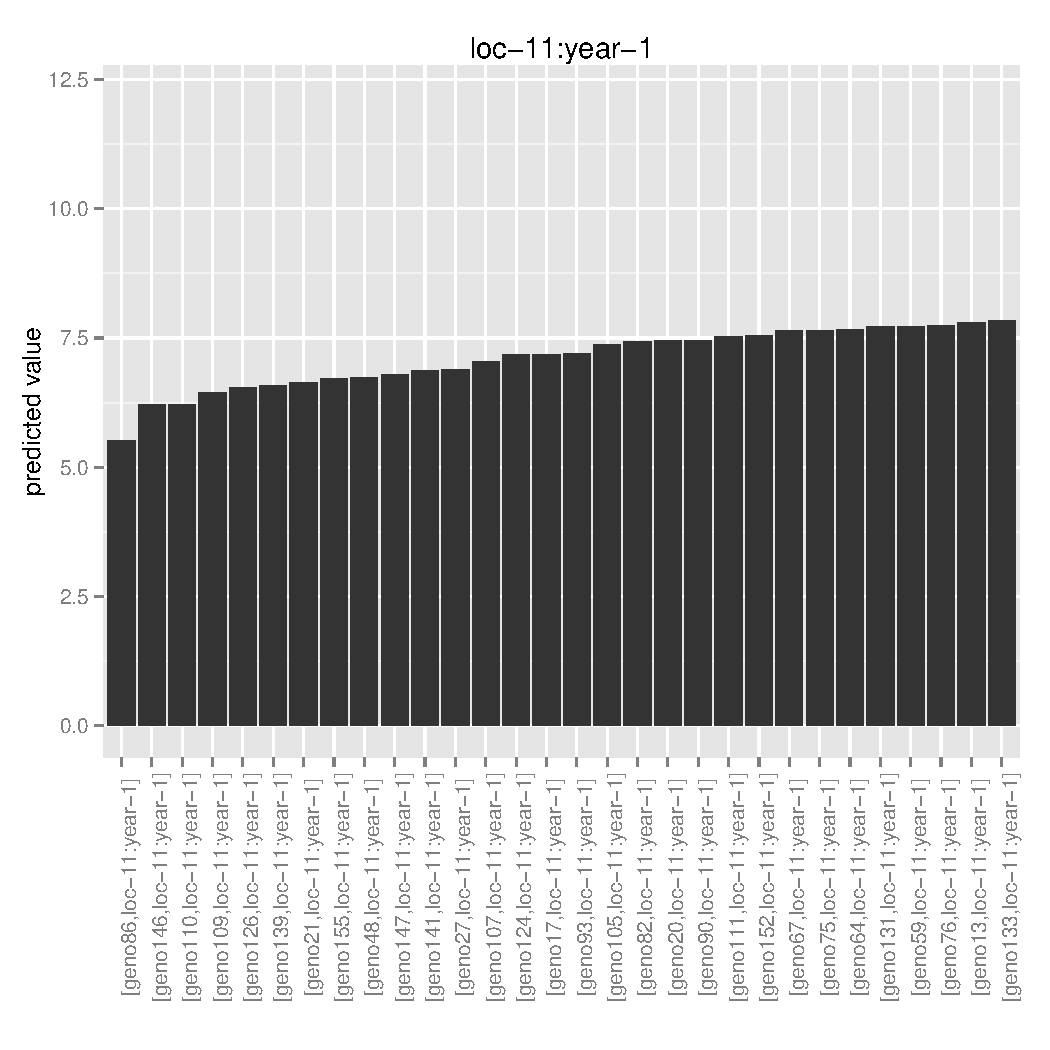
\includegraphics[width=\maxwidth]{figures/PPBstats_unnamed-chunk-53-1} 

}



\end{knitrout}

\item \texttt{beta\_jk} : distribution of each \texttt{beta\_jk} in a list with as many elements as environment. For each element of the list, there are as many graph as needed with \texttt{nb\_parameters\_per\_plot} \texttt{beta\_jk} per graph.
\begin{knitrout}
\definecolor{shadecolor}{rgb}{0.969, 0.969, 0.969}\color{fgcolor}\begin{kframe}
\begin{alltt}
\hlkwd{names}\hlstd{(p_out_check_model_1}\hlopt{$}\hlstd{beta_jk)}
\end{alltt}
\begin{verbatim}
##  [1] "env1-1:2010" "env1-1:2011" "env1-1:2012" "env1-2:2010"
##  [5] "env1-2:2011" "env1-2:2012" "env1-3:2010" "env1-3:2011"
##  [9] "env1-3:2012" "env1-4:2010" "env1-4:2011" "env1-4:2012"
## [13] "env1-5:2011" "env3-1:2011" "env3-1:2012" "env3-2:2011"
## [17] "env3-2:2012" "env3-3:2011"
\end{verbatim}
\begin{alltt}
\hlkwd{names}\hlstd{(p_out_check_model_1}\hlopt{$}\hlstd{beta_jk}\hlopt{$}\hlstd{`env1-1:2010`)}
\end{alltt}
\begin{verbatim}
## [1] "1"
\end{verbatim}
\begin{alltt}
\hlstd{p_out_check_model_1}\hlopt{$}\hlstd{beta_jk}\hlopt{$}\hlstd{`env1-1:2010`}\hlopt{$}\hlstd{`1`}
\end{alltt}
\end{kframe}

{\centering 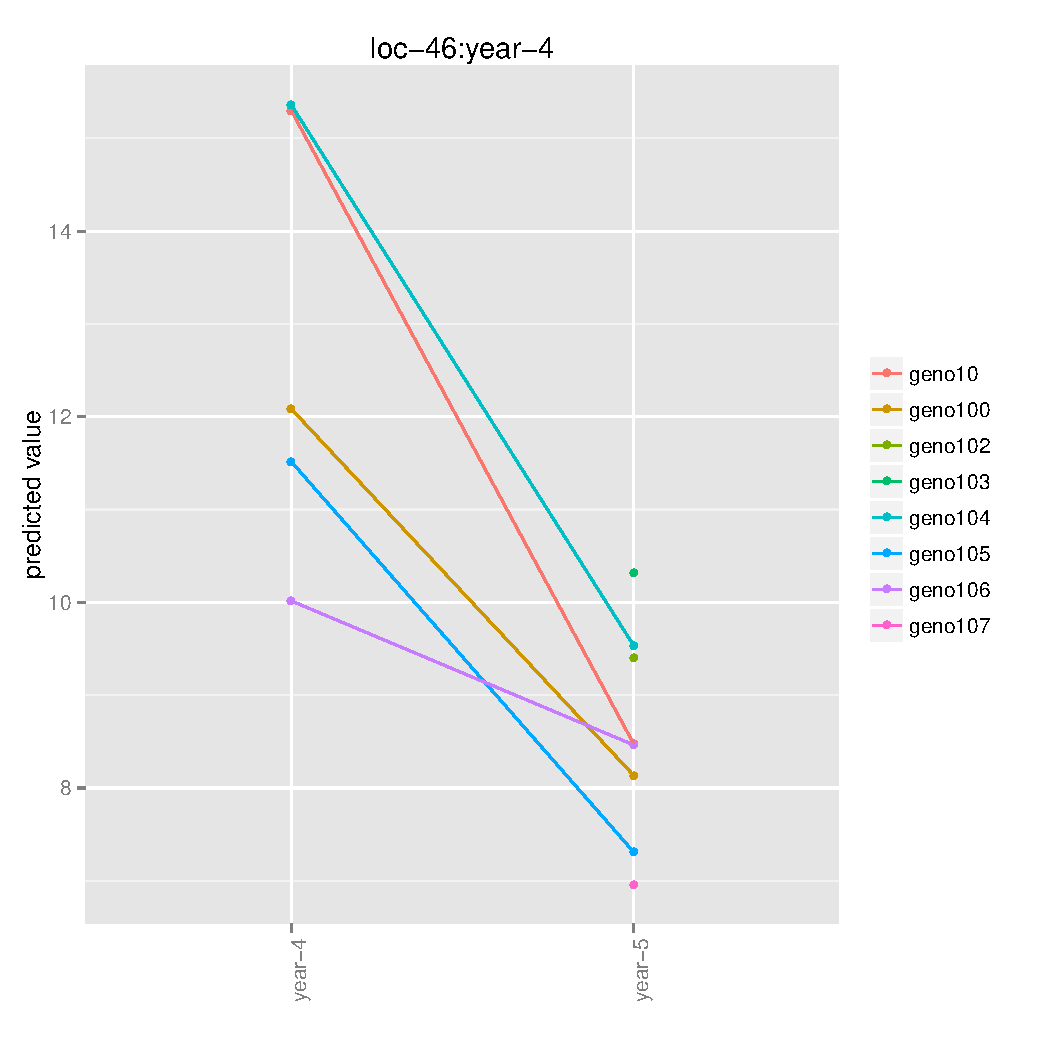
\includegraphics[width=\maxwidth]{figures/PPBstats_unnamed-chunk-54-1} 

}



\end{knitrout}


\item \texttt{sigma\_j} : distribution of each \texttt{sigma\_j}. There are as many graph as needed with \texttt{nb\_parameters\_per\_plot} \texttt{sigma\_j} per graph.
\begin{knitrout}
\definecolor{shadecolor}{rgb}{0.969, 0.969, 0.969}\color{fgcolor}\begin{kframe}
\begin{alltt}
\hlkwd{names}\hlstd{(p_out_check_model_1}\hlopt{$}\hlstd{sigma_j)}
\end{alltt}
\begin{verbatim}
## [1] "1" "2" "3" "4" "5" "6" "7" "8"
\end{verbatim}
\begin{alltt}
\hlstd{p_out_check_model_1}\hlopt{$}\hlstd{sigma_j[[}\hlnum{1}\hlstd{]]}
\end{alltt}
\end{kframe}

{\centering \includegraphics[width=\maxwidth]{figures/PPBstats_unnamed-chunk-55-1} 

}



\end{knitrout}


\item \texttt{epsilon\_ijk} : standardised residuals distribution.
If the model went well it should be between -2 and 2.
\begin{knitrout}
\definecolor{shadecolor}{rgb}{0.969, 0.969, 0.969}\color{fgcolor}\begin{kframe}
\begin{alltt}
\hlstd{p_out_check_model_1}\hlopt{$}\hlstd{epsilon_ijk}
\end{alltt}
\end{kframe}

{\centering \includegraphics[width=\maxwidth]{figures/PPBstats_unnamed-chunk-56-1} 

}



\end{knitrout}

\item \texttt{mcmc\_not\_converge\_traceplot\_density} : a list with the plots of trace and density to check the convergence of the two MCMC only for chains that are not converging thanks to the Gelman-Rubin test. 
If all the chains converge, it is NULL
\begin{knitrout}
\definecolor{shadecolor}{rgb}{0.969, 0.969, 0.969}\color{fgcolor}\begin{kframe}
\begin{alltt}
\hlstd{p_out_check_model_1}\hlopt{$}\hlstd{mcmc_not_converge_traceplot_density}
\end{alltt}
\begin{verbatim}
## NULL
\end{verbatim}
\end{kframe}
\end{knitrout}
Here all the parameters converge.


When considering \texttt{p\_out\_check\_model\_1\_bis}, there is no convergence because the MCMC are too small.

\begin{knitrout}
\definecolor{shadecolor}{rgb}{0.969, 0.969, 0.969}\color{fgcolor}\begin{kframe}
\begin{alltt}
\hlstd{p_out_check_model_1_bis} \hlkwb{=} \hlkwd{get_ggplot}\hlstd{(out_check_model_1_bis)}
\end{alltt}


{\ttfamily\noindent\itshape\color{messagecolor}{\#\# Distribution of sigma\_j in the inverse Gamme distribution are done.}}

{\ttfamily\noindent\itshape\color{messagecolor}{\#\# The mu\_ij posterior distributions are done.}}

{\ttfamily\noindent\itshape\color{messagecolor}{\#\# The beta\_jk posterior distributions are done.}}

{\ttfamily\noindent\itshape\color{messagecolor}{\#\# The sigma\_j posterior distributions are done.}}

{\ttfamily\noindent\itshape\color{messagecolor}{\#\# Trace and density plot for MCMC that did not converged are done.}}\begin{alltt}
\hlstd{p_out_check_model_1_bis}\hlopt{$}\hlstd{mcmc_not_converge_traceplot_density}\hlopt{$}\hlstd{`sigma\textbackslash{}\textbackslash{}[env2-2:2010`}
\end{alltt}
\begin{verbatim}
## $traceplot
## 
## $density
\end{verbatim}
\end{kframe}


{\centering \includegraphics[width=\maxwidth]{figures/PPBstats_unnamed-chunk-58-1} 
\includegraphics[width=\maxwidth]{figures/PPBstats_unnamed-chunk-58-2} 

}



\end{knitrout}

\end{itemize}

Just for fun, you can compare the posterior medians and the arithmetic means for the \texttt{mu\_ij}.

\begin{knitrout}
\definecolor{shadecolor}{rgb}{0.969, 0.969, 0.969}\color{fgcolor}\begin{kframe}
\begin{alltt}
\hlstd{MCMC} \hlkwb{=} \hlstd{out_check_model_1}\hlopt{$}\hlstd{MCMC}
\hlstd{effects} \hlkwb{=} \hlkwd{apply}\hlstd{(MCMC,} \hlnum{2}\hlstd{, median)}
\hlstd{mu_ij_estimated} \hlkwb{=} \hlstd{effects[}\hlkwd{grep}\hlstd{(}\hlstr{"mu"}\hlstd{,}\hlkwd{names}\hlstd{(effects))]}
\hlkwd{names}\hlstd{(mu_ij_estimated)} \hlkwb{=} \hlkwd{sapply}\hlstd{(}\hlkwd{names}\hlstd{(mu_ij_estimated),}
                                \hlkwa{function}\hlstd{(}\hlkwc{x}\hlstd{)\{}  \hlkwd{sub}\hlstd{(}\hlstr{"\textbackslash{}\textbackslash{}]"}\hlstd{,} \hlstr{""}\hlstd{,} \hlkwd{sub}\hlstd{(}\hlstr{"mu\textbackslash{}\textbackslash{}["}\hlstd{,} \hlstr{""}\hlstd{, x)) \}}
                                \hlstd{)}

\hlstd{d} \hlkwb{=} \hlkwd{filter}\hlstd{(data_model_1, location} \hlopt{!=} \hlstr{"env4"}\hlstd{)}
\hlstd{d} \hlkwb{=} \hlkwd{filter}\hlstd{(d, location} \hlopt{!=} \hlstr{"env5"}\hlstd{)}
\hlstd{d} \hlkwb{=} \hlkwd{droplevels}\hlstd{(d)}
\hlstd{environment} \hlkwb{=} \hlkwd{paste}\hlstd{(}\hlkwd{as.character}\hlstd{(d}\hlopt{$}\hlstd{location),} \hlkwd{as.character}\hlstd{(d}\hlopt{$}\hlstd{year),} \hlkwc{sep} \hlstd{=} \hlstr{":"}\hlstd{)}
\hlstd{d}\hlopt{$}\hlstd{entry} \hlkwb{=} \hlkwd{as.factor}\hlstd{(}\hlkwd{paste}\hlstd{(}\hlkwd{as.character}\hlstd{(d}\hlopt{$}\hlstd{germplasm), environment,} \hlkwc{sep} \hlstd{=} \hlstr{","}\hlstd{))}
\hlstd{mu_ij} \hlkwb{=} \hlkwd{tapply}\hlstd{(d}\hlopt{$}\hlstd{mu_ij, d}\hlopt{$}\hlstd{entry, mean,} \hlkwc{na.rm} \hlstd{=} \hlnum{TRUE}\hlstd{)}

\hlstd{check_data} \hlkwb{=} \hlkwd{cbind.data.frame}\hlstd{(mu_ij, mu_ij_estimated[}\hlkwd{names}\hlstd{(mu_ij)])}
\end{alltt}
\end{kframe}
\end{knitrout}

Let's have a look on the relation between the posterior medians and the arithmetic means.
It goes pretty well!

\begin{figure}[H]
\begin{knitrout}
\definecolor{shadecolor}{rgb}{0.969, 0.969, 0.969}\color{fgcolor}\begin{kframe}
\begin{alltt}
\hlstd{p} \hlkwb{=} \hlkwd{ggplot}\hlstd{(check_data,} \hlkwd{aes}\hlstd{(}\hlkwc{x} \hlstd{= mu_ij,} \hlkwc{y} \hlstd{= mu_ij_estimated))}
\hlstd{p} \hlopt{+} \hlkwd{stat_smooth}\hlstd{(}\hlkwc{method} \hlstd{=} \hlstr{"lm"}\hlstd{)} \hlopt{+} \hlkwd{geom_point}\hlstd{()}
\end{alltt}
\end{kframe}

{\centering \includegraphics[width=.6\textwidth]{figures/PPBstats_unnamed-chunk-60-1} 

}



\end{knitrout}
\end{figure}



\subsubsection{Get and visualize mean comparisons}

\paragraph{Get mean comparisons}

Get mean comparisons with \texttt{mean\_comparisons}.
The theory behind mean comparisons are explained in section \ref{mean_comp}.

Below is an example for $\mu$, the same can be done for $\beta$.

\begin{knitrout}
\definecolor{shadecolor}{rgb}{0.969, 0.969, 0.969}\color{fgcolor}\begin{kframe}
\begin{alltt}
\hlcom{# out_mean_comparisons_model_1_mu = mean_comparisons(out_check_model_1, parameter = "mu")}

\hlcom{# Get at least X groups for env2-1:2011. It may take some time ...}
\hlcom{# Get at least X groups for env2-1:2011 is done.}
\hlcom{# Get at least X groups for env2-13:2011. It may take some time ...}
\hlcom{# Get at least X groups for env2-13:2011 is done.}
\hlcom{# Get at least X groups for env2-3:2012. It may take some time ...}
\hlcom{# Get at least X groups for env2-3:2012 is done.}
\hlcom{# Get at least X groups for env2-9:2010. It may take some time ...}
\hlcom{# Get at least X groups for env2-9:2010 is done.}

\hlkwd{load}\hlstd{(}\hlstr{"./data_PPBstats/out_mean_comparisons_model_1_mu.RData"}\hlstd{)} \hlcom{# To save time}
\end{alltt}
\end{kframe}
\end{knitrout}

\texttt{out\_mean\_comparisons\_model\_1\_mu} is a list of three elements:
\begin{itemize}
\item \texttt{data\_mean\_comparisons} a list with as many elements as environment.

\begin{knitrout}
\definecolor{shadecolor}{rgb}{0.969, 0.969, 0.969}\color{fgcolor}\begin{kframe}
\begin{alltt}
\hlkwd{head}\hlstd{(}\hlkwd{names}\hlstd{(out_mean_comparisons_model_1_mu}\hlopt{$}\hlstd{data_mean_comparisons))}
\end{alltt}
\begin{verbatim}
## [1] "env1-1:2010" "env1-1:2011" "env1-1:2012" "env1-2:2010"
## [5] "env1-2:2011" "env1-2:2012"
\end{verbatim}
\end{kframe}
\end{knitrout}

Each element of the list is composed of two elements:

\begin{itemize}
\item \texttt{mean.comparisons}
\begin{knitrout}
\definecolor{shadecolor}{rgb}{0.969, 0.969, 0.969}\color{fgcolor}\begin{kframe}
\begin{alltt}
\hlkwd{head}\hlstd{(out_mean_comparisons_model_1_mu}\hlopt{$}\hlstd{data_mean_comparisons}\hlopt{$}\hlstd{`env1-1:2010`}\hlopt{$}\hlstd{mean.comparisons)}
\end{alltt}
\begin{verbatim}
##                parameter   median groups nb_group alpha
## 1 mu[pop-11,env1-1:2010] 38.43108      a       10  0.05
## 2  mu[pop-1,env1-1:2010] 41.69727     ab       10  0.05
## 3 mu[pop-18,env1-1:2010] 45.84213    abc       10  0.05
## 4  mu[pop-3,env1-1:2010] 47.71686   abcd       10  0.05
## 5 mu[pop-10,env1-1:2010] 48.10493  abcde       10  0.05
## 6  mu[pop-4,env1-1:2010] 49.18758 abcdef       10  0.05
##   alpha.correction  entry environment location year
## 1        soft.bonf pop-11 env1-1:2010   env1-1 2010
## 2        soft.bonf  pop-1 env1-1:2010   env1-1 2010
## 3        soft.bonf pop-18 env1-1:2010   env1-1 2010
## 4        soft.bonf  pop-3 env1-1:2010   env1-1 2010
## 5        soft.bonf pop-10 env1-1:2010   env1-1 2010
## 6        soft.bonf  pop-4 env1-1:2010   env1-1 2010
\end{verbatim}
\end{kframe}
\end{knitrout}

\item \texttt{Mpvalue} : a square matrix with pvalue computed for each pair of parameter.
\begin{knitrout}
\definecolor{shadecolor}{rgb}{0.969, 0.969, 0.969}\color{fgcolor}\begin{kframe}
\begin{alltt}
\hlstd{out_mean_comparisons_model_1_mu}\hlopt{$}\hlstd{data_mean_comparisons}\hlopt{$}\hlstd{`env1-1:2010`}\hlopt{$}\hlstd{Mpvalue[}\hlnum{1}\hlopt{:}\hlnum{3}\hlstd{,} \hlnum{1}\hlopt{:}\hlnum{3}\hlstd{]}
\end{alltt}
\begin{verbatim}
##                        mu[pop-11,env1-1:2010] mu[pop-1,env1-1:2010]
## mu[pop-11,env1-1:2010]                      0               0.17555
## mu[pop-1,env1-1:2010]                       0               0.00000
## mu[pop-18,env1-1:2010]                      0               0.00000
##                        mu[pop-18,env1-1:2010]
## mu[pop-11,env1-1:2010]                 0.0402
## mu[pop-1,env1-1:2010]                  0.1524
## mu[pop-18,env1-1:2010]                 0.0000
\end{verbatim}
\end{kframe}
\end{knitrout}

\end{itemize}

\item \texttt{data\_env\_with\_no\_controls} a list with as many elements as environment.
\begin{knitrout}
\definecolor{shadecolor}{rgb}{0.969, 0.969, 0.969}\color{fgcolor}\begin{kframe}
\begin{alltt}
\hlkwd{names}\hlstd{(out_mean_comparisons_model_1_mu}\hlopt{$}\hlstd{data_env_with_no_controls)}
\end{alltt}
\begin{verbatim}
## [1] "env5:2010"
\end{verbatim}
\end{kframe}
\end{knitrout}

In each list it is mean.comparisons
\begin{knitrout}
\definecolor{shadecolor}{rgb}{0.969, 0.969, 0.969}\color{fgcolor}\begin{kframe}
\begin{alltt}
\hlkwd{head}\hlstd{(out_mean_comparisons_model_1_mu}\hlopt{$}\hlstd{data_env_with_no_controls}\hlopt{$}\hlstd{`env5:2010`}\hlopt{$}\hlstd{mean.comparisons)}
\end{alltt}
\begin{verbatim}
##             entry germplasm environment block X Y   median
## 1 pop-1,env5:2010     pop-1   env5:2010     1 3 c 42.32750
## 2 pop-2,env5:2010     pop-2   env5:2010     1 4 d 38.02544
## 3 pop-3,env5:2010     pop-3   env5:2010     1 5 e 44.49495
## 4 pop-4,env5:2010     pop-4   env5:2010     1 6 f 44.46948
## 5 pop-5,env5:2010     pop-5   env5:2010     1 7 g 35.77590
## 6 pop-6,env5:2010     pop-6   env5:2010     1 8 h 36.59313
##             parameter location year
## 1 mu[pop-1,env5:2010]     env5 2010
## 2 mu[pop-2,env5:2010]     env5 2010
## 3 mu[pop-3,env5:2010]     env5 2010
## 4 mu[pop-4,env5:2010]     env5 2010
## 5 mu[pop-5,env5:2010]     env5 2010
## 6 mu[pop-6,env5:2010]     env5 2010
\end{verbatim}
\end{kframe}
\end{knitrout}

\item \texttt{data\_env\_whose\_param\_did\_not\_converge} a list with as many elements as environment.
\begin{knitrout}
\definecolor{shadecolor}{rgb}{0.969, 0.969, 0.969}\color{fgcolor}\begin{kframe}
\begin{alltt}
\hlkwd{names}\hlstd{(out_mean_comparisons_model_1_mu}\hlopt{$}\hlstd{data_env_whose_param_did_not_converge)}
\end{alltt}
\begin{verbatim}
## NULL
\end{verbatim}
\end{kframe}
\end{knitrout}
Here it is NULL as all parameters converge. 
Otherwise in each list it is mean.comparisons.
\begin{knitrout}
\definecolor{shadecolor}{rgb}{0.969, 0.969, 0.969}\color{fgcolor}\begin{kframe}
\begin{alltt}
\hlkwd{head}\hlstd{(out_mean_comparisons_model_1_mu}\hlopt{$}\hlstd{data_env_with_no_controls}\hlopt{$}\hlstd{`env5:2010`}\hlopt{$}\hlstd{mean.comparisons)}
\end{alltt}
\begin{verbatim}
##             entry germplasm environment block X Y   median
## 1 pop-1,env5:2010     pop-1   env5:2010     1 3 c 42.32750
## 2 pop-2,env5:2010     pop-2   env5:2010     1 4 d 38.02544
## 3 pop-3,env5:2010     pop-3   env5:2010     1 5 e 44.49495
## 4 pop-4,env5:2010     pop-4   env5:2010     1 6 f 44.46948
## 5 pop-5,env5:2010     pop-5   env5:2010     1 7 g 35.77590
## 6 pop-6,env5:2010     pop-6   env5:2010     1 8 h 36.59313
##             parameter location year
## 1 mu[pop-1,env5:2010]     env5 2010
## 2 mu[pop-2,env5:2010]     env5 2010
## 3 mu[pop-3,env5:2010]     env5 2010
## 4 mu[pop-4,env5:2010]     env5 2010
## 5 mu[pop-5,env5:2010]     env5 2010
## 6 mu[pop-6,env5:2010]     env5 2010
\end{verbatim}
\end{kframe}
\end{knitrout}

\end{itemize}


\paragraph{Visualize mean comparisons}

To see the output, use \texttt{get\_ggplot}.
On each plot, the \texttt{alpha} (type one error) value and the alpha correction are displayed.
\texttt{alpha = Imp} means that no differences were possible to find.
For \texttt{ggplot.type = "interaction"} and \texttt{ggplot.type = "score"}, it is display under the form: \texttt{alpha | alpha correction}.

The ggplot are done for each element of the list coming rom \texttt{mean\_comparisons}.

For each ggplot.type, it is a list of three elements being lists with as many elements as environment. 

For each element of the list, there are as many graph as needed with \texttt{nb\_parameters\_per\_plot} parameters per graph.

\subparagraph{barplot}

\begin{knitrout}
\definecolor{shadecolor}{rgb}{0.969, 0.969, 0.969}\color{fgcolor}\begin{kframe}
\begin{alltt}
\hlstd{p_barplot_mu} \hlkwb{=} \hlkwd{get_ggplot}\hlstd{(out_mean_comparisons_model_1_mu,} \hlkwc{ggplot.type} \hlstd{=} \hlstr{"barplot"}\hlstd{)}
\hlkwd{names}\hlstd{(p_barplot_mu)}
\end{alltt}
\begin{verbatim}
## [1] "data_mean_comparisons"                
## [2] "data_env_with_no_controls"            
## [3] "data_env_whose_param_did_not_converge"
\end{verbatim}
\end{kframe}
\end{knitrout}

From \texttt{data\_mean\_comparisons}, only environments where all MCMC converge are represented.

Letters are displayed on each bar. Parameters that do not share the same letters are different regarding type I error (alpha) and alpha correction. 

The error I (alpha) and the alpha correction are displayed in the title. 
alpha = Imp means that no differences were possible to find.

\begin{knitrout}
\definecolor{shadecolor}{rgb}{0.969, 0.969, 0.969}\color{fgcolor}\begin{kframe}
\begin{alltt}
\hlstd{p} \hlkwb{=} \hlstd{p_barplot_mu}\hlopt{$}\hlstd{data_mean_comparisons}

\hlkwd{head}\hlstd{(}\hlkwd{names}\hlstd{(p))}
\end{alltt}
\begin{verbatim}
## [1] "env1-1:2010" "env1-1:2011" "env1-1:2012" "env1-2:2010"
## [5] "env1-2:2011" "env1-2:2012"
\end{verbatim}
\begin{alltt}
\hlstd{p_env} \hlkwb{=} \hlstd{p}\hlopt{$}\hlstd{`env1-1:2010`}
\hlkwd{names}\hlstd{(p_env)}
\end{alltt}
\begin{verbatim}
## [1] "1" "2" "3" "4"
\end{verbatim}
\begin{alltt}
\hlstd{p_env}\hlopt{$}\hlstd{`1`}
\hlstd{p_env}\hlopt{$}\hlstd{`2`}
\hlstd{p_env}\hlopt{$}\hlstd{`3`}
\hlstd{p_env}\hlopt{$}\hlstd{`4`}
\end{alltt}
\end{kframe}

{\centering \includegraphics[width=\maxwidth]{figures/PPBstats_unnamed-chunk-70-1} 
\includegraphics[width=\maxwidth]{figures/PPBstats_unnamed-chunk-70-2} 
\includegraphics[width=\maxwidth]{figures/PPBstats_unnamed-chunk-70-3} 
\includegraphics[width=\maxwidth]{figures/PPBstats_unnamed-chunk-70-4} 

}



\end{knitrout}

For \texttt{data\_env\_with\_no\_controls}, only environments where there were no controls are represented.

\begin{knitrout}
\definecolor{shadecolor}{rgb}{0.969, 0.969, 0.969}\color{fgcolor}\begin{kframe}
\begin{alltt}
\hlstd{p_barplot_mu}\hlopt{$}\hlstd{data_env_with_no_controls}
\end{alltt}
\begin{verbatim}
## $`env5:2010`
## $`env5:2010`$`1`
\end{verbatim}
\end{kframe}



{\centering \includegraphics[width=\maxwidth]{figures/PPBstats_unnamed-chunk-71-1} 

}



\end{knitrout}


For \texttt{data\_env\_whose\_param\_did\_not\_converge}, only environments where MCMC did not converge are represented.

\begin{knitrout}
\definecolor{shadecolor}{rgb}{0.969, 0.969, 0.969}\color{fgcolor}\begin{kframe}
\begin{alltt}
\hlstd{p_barplot_mu}\hlopt{$}\hlstd{data_env_whose_param_did_not_converge}
\end{alltt}
\begin{verbatim}
## list()
\end{verbatim}
\end{kframe}
\end{knitrout}


Regarding pairs of entries in a given environment, 
it is possible to get comparison of paris of entries in a given location.
This is useful if you want to compare two versions within a group.
For exemple:
\begin{knitrout}
\definecolor{shadecolor}{rgb}{0.969, 0.969, 0.969}\color{fgcolor}\begin{kframe}
\begin{alltt}
\hlkwd{data}\hlstd{(data_version)}
\hlkwd{head}\hlstd{(data_version)}
\end{alltt}
\begin{verbatim}
##   year location germplasm group version
## 1 2010   env1-1     tem-1     1      v1
## 2 2010   env1-1     tem-2     1      v2
## 3 2010   env1-1     pop-1     2      v1
## 4 2010   env1-1     pop-2     2      v2
## 5 2010   env1-2     tem-1     3      v1
## 6 2010   env1-2     tem-2     3      v2
\end{verbatim}
\end{kframe}
\end{knitrout}

Here, in location \texttt{env1-1}, \texttt{tem-1} and \texttt{tem-2} are two version belonging to the same groupe.

Lets' make the plots:
\begin{knitrout}
\definecolor{shadecolor}{rgb}{0.969, 0.969, 0.969}\color{fgcolor}\begin{kframe}
\begin{alltt}
\hlstd{p_barplot_mu_version} \hlkwb{=} \hlkwd{get_ggplot}\hlstd{(out_mean_comparisons_model_1_mu,} \hlkwc{data_version} \hlstd{= data_version,} \hlkwc{ggplot.type} \hlstd{=} \hlstr{"barplot"}\hlstd{)}
\end{alltt}


{\ttfamily\noindent\color{warningcolor}{\#\# Warning in FUN(X[[i]], ...): data\_mean\_comparisons: the following environments in data\_version are not taken: env5:2010.}}

{\ttfamily\noindent\color{warningcolor}{\#\# Warning in FUN(X[[i]], ...): data\_env\_with\_no\_controls: the following environments in data\_version are not taken: env1-1:2010, env1-2:2010, env1-1:2012.}}

{\ttfamily\noindent\color{warningcolor}{\#\# Warning in FUN(X[[i]], ...): data\_env\_with\_no\_controls: no t.test are done as there are not enough observations.}}

{\ttfamily\noindent\color{warningcolor}{\#\# Warning in FUN(X[[i]], ...): data\_env\_whose\_param\_did\_not\_converge: the following environments in data\_version are not taken: env1-1:2010, env1-2:2010, env1-1:2012, env5:2010.}}

{\ttfamily\noindent\color{warningcolor}{\#\# Warning in FUN(X[[i]], ...): data\_env\_whose\_param\_did\_not\_converge: there are no environment to display}}\begin{alltt}
\hlstd{p_barplot_mu_version}\hlopt{$}\hlstd{data_mean_comparisons}\hlopt{$}\hlstd{`env1-1:2010`}
\end{alltt}
\begin{verbatim}
## $`1`
\end{verbatim}
\end{kframe}


{\centering \includegraphics[width=\maxwidth]{figures/PPBstats_unnamed-chunk-74-1} 

}



\end{knitrout}

The stars corresponds to the pvalue:

\begin{center}
\begin{tabular}{cc}
\hline
pvalue & stars \\
\hline
$< 0.001$ & *** \\
$[0.001 , 0.05]$ & ** \\
$[0.05 , 0.01]$ & * \\
$> 0.01$ & . \\
\hline
\end{tabular}
\end{center}

The pvalue is computed as describe in section \ref{mean_comp} if the parameters have been estimated with the model.

For environments where MCMC did not converge or without environments, it is a \texttt{t.test} which is perform.

\begin{knitrout}
\definecolor{shadecolor}{rgb}{0.969, 0.969, 0.969}\color{fgcolor}\begin{kframe}
\begin{alltt}
\hlstd{p_barplot_mu_version}\hlopt{$}\hlstd{data_env_with_no_controls}
\end{alltt}
\begin{verbatim}
## $`env5:2010`
## $`env5:2010`$`1`
\end{verbatim}
\end{kframe}



{\centering \includegraphics[width=.6\textwidth]{figures/PPBstats_unnamed-chunk-75-1} 

}



\end{knitrout}

\begin{knitrout}
\definecolor{shadecolor}{rgb}{0.969, 0.969, 0.969}\color{fgcolor}\begin{kframe}
\begin{alltt}
\hlstd{p_barplot_mu_version}\hlopt{$}\hlstd{data_env_whose_param_did_not_converge}
\end{alltt}
\begin{verbatim}
## NULL
\end{verbatim}
\end{kframe}
\end{knitrout}

\subparagraph{interaction}

With \texttt{ggplot.type = "interaction"}, you can display the year effect as well as detect groups.
One group is represented by one vertical line.
Germplasms which share the same group are not different.
Germplasms which do not share the same groupe are different (section \ref{mean_comp}).

The ggplot are done for each element of the list coming rom \texttt{mean\_comparisons}.

For each ggplot.type, it is a list of three elements being lists with as many elements as environment. 

For each element of the list, there are as many graph as needed with \texttt{nb\_parameters\_per\_plot} parameters per graph.


\begin{knitrout}
\definecolor{shadecolor}{rgb}{0.969, 0.969, 0.969}\color{fgcolor}\begin{kframe}
\begin{alltt}
\hlstd{p_interaction} \hlkwb{=} \hlkwd{get_ggplot}\hlstd{(out_mean_comparisons_model_1_mu,} \hlkwc{ggplot.type} \hlstd{=} \hlstr{"interaction"}\hlstd{)}

\hlkwd{head}\hlstd{(}\hlkwd{names}\hlstd{(p_interaction}\hlopt{$}\hlstd{data_mean_comparisons))}
\end{alltt}
\begin{verbatim}
## [1] "env1-1" "env1-2" "env1-3" "env1-4" "env1-5" "env2-1"
\end{verbatim}
\begin{alltt}
\hlstd{p_env} \hlkwb{=} \hlstd{p_interaction}\hlopt{$}\hlstd{data_mean_comparisons}\hlopt{$}\hlstd{`env1-1`}
\hlkwd{names}\hlstd{(p_env)}
\end{alltt}
\begin{verbatim}
## [1] "1" "2" "3" "4"
\end{verbatim}
\begin{alltt}
\hlstd{p_env}\hlopt{$}\hlstd{`1`}
\hlstd{p_env}\hlopt{$}\hlstd{`2`}
\hlstd{p_env}\hlopt{$}\hlstd{`3`}
\hlstd{p_env}\hlopt{$}\hlstd{`4`}
\end{alltt}
\end{kframe}

{\centering \includegraphics[width=\maxwidth]{figures/PPBstats_unnamed-chunk-77-1} 
\includegraphics[width=\maxwidth]{figures/PPBstats_unnamed-chunk-77-2} 
\includegraphics[width=\maxwidth]{figures/PPBstats_unnamed-chunk-77-3} 
\includegraphics[width=\maxwidth]{figures/PPBstats_unnamed-chunk-77-4} 

}



\end{knitrout}


\subparagraph{score}

For the score, more entries are displayed.
An high score means that the entry was in a group with an high mean.
A low socre means that the entry was in a group with an low mean.
This plot is useful to look at year effects.

\begin{knitrout}
\definecolor{shadecolor}{rgb}{0.969, 0.969, 0.969}\color{fgcolor}\begin{kframe}
\begin{alltt}
\hlstd{p_score} \hlkwb{=} \hlkwd{get_ggplot}\hlstd{(out_mean_comparisons_model_1_mu,} \hlkwc{ggplot.type} \hlstd{=} \hlstr{"score"}\hlstd{)}

\hlkwd{head}\hlstd{(}\hlkwd{names}\hlstd{(p_score))}
\end{alltt}
\begin{verbatim}
## [1] "env1-1" "env1-2" "env1-3" "env1-4" "env1-5" "env2-1"
\end{verbatim}
\begin{alltt}
\hlstd{p_env} \hlkwb{=} \hlstd{p_score}\hlopt{$}\hlstd{`env1-1`}
\hlkwd{names}\hlstd{(p_env)}
\end{alltt}
\begin{verbatim}
## [1] "1" "2" "3" "4"
\end{verbatim}
\begin{alltt}
\hlstd{p_env}\hlopt{$}\hlstd{`1`}
\hlstd{p_env}\hlopt{$}\hlstd{`2`}
\hlstd{p_env}\hlopt{$}\hlstd{`3`}
\hlstd{p_env}\hlopt{$}\hlstd{`4`}
\end{alltt}
\end{kframe}

{\centering \includegraphics[width=\maxwidth]{figures/PPBstats_unnamed-chunk-78-1} 
\includegraphics[width=\maxwidth]{figures/PPBstats_unnamed-chunk-78-2} 
\includegraphics[width=\maxwidth]{figures/PPBstats_unnamed-chunk-78-3} 
\includegraphics[width=\maxwidth]{figures/PPBstats_unnamed-chunk-78-4} 

}



\end{knitrout}


\newpage

\section{Family of analysis 2 : germplasm, location, year, environment, and interaction effects in a network of farms}


\subsection{AMMI}
\label{ammi}

\subsubsection{Theory of the model}

The Additive Main effects and Multiplicative Interaction (AMMI) model is based on two analyses \citep{gauch_statistical_2006} : 
\begin{enumerate}

\item an \textbf{ANOVA} with the following model :

\begin{equation}
Y_{ijk} = \mu + \alpha_{i} + \theta_{j} + rep_{k}(\theta_{j}) + \eta_{i}\nu_{j} + \varepsilon_{ijk}; \quad \varepsilon_{ijk} \sim \mathcal{N} (0,\sigma^2)
\label{ammi_anova}
\end{equation}

With,

\begin{tabular}{ll}
$Y_{ijk}$ & the phenotypic value for replication $k$, germplasm $i$ and location $j$, \\
$\mu$ & the general mean, \\
$\alpha_{i}$ & the germplasm $i$ effect, \\
$\theta_{j}$ & location $j$ effect, \\
$rep_{k}(\theta_{j})$ & the replication $k$ nested in location effect, \\
$\eta_{i}\nu_{j}$ & the germplasm $\times$ location effect, \\
$\varepsilon_{ijk}$ & the residuals.\\
\end{tabular}

~\\ 

Or, if there are several years in the data set:

\begin{equation}
Y_{ijkl} = \mu + \alpha_{i} + \theta_{j} + rep_{k}(\theta_{j}\beta_{l}) + \eta_{i}\nu_{j} + 
\beta_{l} + \beta_{l}\alpha_{i} + \beta_{l}\theta_{j} + 
\varepsilon_{ijk}; \quad \varepsilon_{ijk} \sim \mathcal{N} (0,\sigma^2)
\label{ammi_anova}
\end{equation}

With,

\begin{tabular}{ll}
$Y_{ijkl}$ & the phenotypic value for replication $k$, germplasm $i$, location $j$ and year $l$, \\
$\mu$ & the general mean, \\
$\alpha_{i}$ & the germplasm $i$ effect, \\
$\theta_{j}$ & location $j$ effect, \\
$rep_{k}(\theta_{j}\beta_{l})$ & the replication $k$ nested in location and year effect, \\
$\eta_{i}\nu_{j}$ & the germplasm $\times$ location effect, \\
$\beta_{l}$ & the year $l$ effect, \\
$\beta_{l}\alpha_{i}$ & the year $\times$ germplasm interaction effect, \\
$\beta_{l}\theta_{j}$ & the year $\times$ location interaction effect, \\
$\varepsilon_{ijk}$ & the residuals.\\
\end{tabular}


\item a \textbf{PCA} which analyse deeper the germplasm $\times$ location interaction: 

\begin{displaymath}
\eta_{i}\nu_{j} = \sum_{n}^{N} \lambda_{n} \gamma_{in} \omega_{jn}
\end{displaymath}

which can also be written:

\begin{displaymath}
\eta_{i}\nu_{j} = \sum_{n}^{N} (\sqrt{\lambda_{n}} \gamma_{in}) (\sqrt{\lambda_{n}} \omega_{jn})
\end{displaymath}


With,

\begin{tabular}{ll}
$\eta_{i}\nu_{j}$ & interaction of germplasm $i$ with location $j$, \\
$N$ & the number of dimension (PCA componant) which has as maximum value the number of location, \\
$\lambda_{n}$ & the eigen value for componant $n$, \\
$\gamma_{in}$ & eigen vector for germplasm $i$ for componant $n$, \\
$\omega_{jn}$ & eigen vector for  location $j$  for componant $n$. \\
\end{tabular}


The data are double centered on location and germplasm.
The PCA study the structure of the interaction matrix.
The location are the variable and the germplasm are the individuals.

This PCA allows to detect
\begin{itemize}
\item germplasm that are stable (i.e. contribute less to interaction)
\item which germplasm interact the most with which location
\item which location have the same profile regarding interaction
\end{itemize}

\end{enumerate}


\subsubsection{Steps with \pack}

For AMMI analysis, you can follow these steps (Figure \ref{main_workflow}):

\begin{enumerate}
\item Run the model with \texttt{GxE} and \texttt{gxe\_analysis = "AMMI"}
\item Check model outputs with graphs to know if you can continue the analysis with \texttt{check\_model}
\item Get mean comparisons for each factor with \texttt{mean\_comparisons} and vizualise it with \texttt{get\_ggplot}
\item Get groups of each parameters with \texttt{parameters\_groups} and visualise it with \texttt{get\_ggplot}
\end{enumerate}

Let's get the data.

\begin{knitrout}
\definecolor{shadecolor}{rgb}{0.969, 0.969, 0.969}\color{fgcolor}\begin{kframe}
\begin{alltt}
\hlkwd{data}\hlstd{(data_GxE)}
\hlkwd{head}\hlstd{(data_GxE)}
\end{alltt}
\begin{verbatim}
##   location year germplasm block X Y       y1       y2       y3
## 1       L1 2016    germ:2     1 A 1 14.32724 41.85377 66.05498
## 2       L1 2016    germ:1     1 A 2 23.03428 37.38970 63.39528
## 3       L1 2016    germ:7     1 A 3 24.91349 38.38628 60.52710
## 4       L1 2016    germ:3     1 A 4 24.99078 39.72205 60.80393
## 5       L1 2016   germ:14     1 A 5 18.95340 46.60443 53.71210
## 6       L1 2016   germ:12     1 B 1 21.31660 49.94656 60.71978
\end{verbatim}
\end{kframe}
\end{knitrout}


\subsubsection{Run the model}
To run model GxE on the dataset, used the function \texttt{GxE}.
You can run it on one variable.

\begin{knitrout}
\definecolor{shadecolor}{rgb}{0.969, 0.969, 0.969}\color{fgcolor}\begin{kframe}
\begin{alltt}
\hlstd{out_ammi} \hlkwb{=} \hlkwd{GxE}\hlstd{(data_GxE,} \hlkwc{variable} \hlstd{=} \hlstr{"y1"}\hlstd{,} \hlkwc{gxe_analysis} \hlstd{=} \hlstr{"AMMI"}\hlstd{)}
\end{alltt}


{\ttfamily\noindent\itshape\color{messagecolor}{\#\# AMMI model done for y1}}\end{kframe}
\end{knitrout}


\texttt{out\_ammi} is a list containing three elements :

\begin{itemize}
\item \texttt{info} : a list with variable and gxe\_analysis
\begin{knitrout}
\definecolor{shadecolor}{rgb}{0.969, 0.969, 0.969}\color{fgcolor}\begin{kframe}
\begin{alltt}
\hlstd{out_ammi}\hlopt{$}\hlstd{info}
\end{alltt}
\begin{verbatim}
## $variable
## [1] "y1"
## 
## $gxe_analysis
## [1] "AMMI"
\end{verbatim}
\end{kframe}
\end{knitrout}
\item \texttt{ANOVA} a list with five elements :
  \begin{itemize}
  \item \texttt{model}
\begin{knitrout}
\definecolor{shadecolor}{rgb}{0.969, 0.969, 0.969}\color{fgcolor}\begin{kframe}
\begin{alltt}
\hlstd{out_ammi}\hlopt{$}\hlstd{ANOVA}\hlopt{$}\hlstd{model}
\end{alltt}
\begin{verbatim}
## 
## Call:
## lm(formula = variable ~ germplasm * location + block_in_env, 
##     data = data)
## 
## Coefficients:
##           (Intercept)             germplasm1  
##              20.70849                0.50554  
##            germplasm2             germplasm3  
##              -2.08334               -0.38939  
##            germplasm4             germplasm5  
##               1.09734               -1.19621  
##            germplasm6             germplasm7  
##               0.16386                0.72661  
##            germplasm8             germplasm9  
##               1.49549                1.78775  
##           germplasm10            germplasm11  
##               0.63312               -1.20916  
##           germplasm12            germplasm13  
##               0.29679                0.35626  
##           germplasm14            germplasm15  
##               1.33065               -1.52504  
##           germplasm16            germplasm17  
##              -0.56769               -0.73263  
##           germplasm18            germplasm19  
##              -0.34611                0.37692  
##             location1              location2  
##               0.72717                4.76131  
##         block_in_env1          block_in_env2  
##              -2.10792               -0.30555  
##         block_in_env3          block_in_env4  
##              -0.18481               -1.39800  
##         block_in_env5          block_in_env6  
##               0.66418                2.25382  
##         block_in_env7          block_in_env8  
##                    NA                     NA  
##  germplasm1:location1   germplasm2:location1  
##               1.09629               -3.67906  
##  germplasm3:location1   germplasm4:location1  
##               0.86540                0.33758  
##  germplasm5:location1   germplasm6:location1  
##              -0.35726                0.72636  
##  germplasm7:location1   germplasm8:location1  
##              -0.33219               -0.33242  
##  germplasm9:location1  germplasm10:location1  
##              -0.06286               -0.60915  
## germplasm11:location1  germplasm12:location1  
##               0.81094                0.91505  
## germplasm13:location1  germplasm14:location1  
##               0.70964                2.42945  
## germplasm15:location1  germplasm16:location1  
##              -3.58258               -0.35926  
## germplasm17:location1  germplasm18:location1  
##               3.36809                0.77027  
## germplasm19:location1   germplasm1:location2  
##               1.18556               -2.03698  
##  germplasm2:location2   germplasm3:location2  
##              -0.43476                1.83102  
##  germplasm4:location2   germplasm5:location2  
##              -1.18392                3.30243  
##  germplasm6:location2   germplasm7:location2  
##              -2.87038                2.27662  
##  germplasm8:location2   germplasm9:location2  
##               0.89072                0.31439  
## germplasm10:location2  germplasm11:location2  
##              -1.15072               -2.28962  
## germplasm12:location2  germplasm13:location2  
##              -3.06243                3.82029  
## germplasm14:location2  germplasm15:location2  
##              -1.85852                0.06938  
## germplasm16:location2  germplasm17:location2  
##               4.47337               -1.71149  
## germplasm18:location2  germplasm19:location2  
##              -1.52013               -0.40986
\end{verbatim}
\end{kframe}
\end{knitrout}
  \item \texttt{anova\_model}
\begin{knitrout}
\definecolor{shadecolor}{rgb}{0.969, 0.969, 0.969}\color{fgcolor}\begin{kframe}
\begin{alltt}
\hlstd{out_ammi}\hlopt{$}\hlstd{ANOVA}\hlopt{$}\hlstd{anova_model}
\end{alltt}
\begin{verbatim}
## Analysis of Variance Table
## 
## Response: variable
##                     Df  Sum Sq Mean Sq F value   Pr(>F)    
## germplasm           19  190.66   10.03  0.3712   0.9921    
## location             2 2623.54 1311.77 48.5185 5.69e-16 ***
## block_in_env         6  115.34   19.22  0.7110   0.6414    
## germplasm:location  38  825.18   21.72  0.8032   0.7778    
## Residuals          114 3082.16   27.04                     
## ---
## Signif. codes:  0 '***' 0.001 '**' 0.01 '*' 0.05 '.' 0.1 ' ' 1
\end{verbatim}
\end{kframe}
\end{knitrout}
  \item \texttt{germplasm\_effects} a list of two elements :
    \begin{itemize}
    \item \texttt{effects}
\begin{knitrout}
\definecolor{shadecolor}{rgb}{0.969, 0.969, 0.969}\color{fgcolor}\begin{kframe}
\begin{alltt}
\hlstd{out_ammi}\hlopt{$}\hlstd{ANOVA}\hlopt{$}\hlstd{germplasm_effects}\hlopt{$}\hlstd{effects}
\end{alltt}
\begin{verbatim}
##     germ:1    germ:10    germ:11    germ:12    germ:13    germ:14 
##  0.5055402 -2.0833355 -0.3893941  1.0973419 -1.1962053  0.1638570 
##    germ:15    germ:16    germ:17    germ:18    germ:19     germ:2 
##  0.7266050  1.4954919  1.7877499  0.6331183 -1.2091564  0.2967890 
##    germ:20     germ:3     germ:4     germ:5     germ:6     germ:7 
##  0.3562593  1.3306487 -1.5250386 -0.5676933 -0.7326310 -0.3461143 
##     germ:8     germ:9 
##  0.3769158 -0.7207485
\end{verbatim}
\end{kframe}
\end{knitrout}
    \item \texttt{intra\_variance}
\begin{knitrout}
\definecolor{shadecolor}{rgb}{0.969, 0.969, 0.969}\color{fgcolor}\begin{kframe}
\begin{alltt}
\hlstd{out_ammi}\hlopt{$}\hlstd{ANOVA}\hlopt{$}\hlstd{germplasm_effects}\hlopt{$}\hlstd{intra_variance}
\end{alltt}
\begin{verbatim}
##    germ:1   germ:10   germ:11   germ:12   germ:13   germ:14 
## 15.965283  3.196085 16.472166 23.173849 17.368449  6.871368 
##   germ:15   germ:16   germ:17   germ:18   germ:19    germ:2 
## 20.497187 24.386542 14.210313 57.489583 20.790956 28.830542 
##   germ:20    germ:3    germ:4    germ:5    germ:6    germ:7 
## 26.605904 23.161228 17.215151 12.059959 11.686595  9.479899 
##    germ:8    germ:9 
## 28.873479  6.935395
\end{verbatim}
\end{kframe}
\end{knitrout}
    \end{itemize}
  \item \texttt{location\_effects}
\begin{knitrout}
\definecolor{shadecolor}{rgb}{0.969, 0.969, 0.969}\color{fgcolor}\begin{kframe}
\begin{alltt}
\hlstd{out_ammi}\hlopt{$}\hlstd{ANOVA}\hlopt{$}\hlstd{location_effects}\hlopt{$}\hlstd{effects}
\end{alltt}
\begin{verbatim}
##         L1         L2         L3 
##  0.7271695  4.7613066 -5.4884761
\end{verbatim}
\end{kframe}
\end{knitrout}
  \item \texttt{interaction\_matrix}
\begin{knitrout}
\definecolor{shadecolor}{rgb}{0.969, 0.969, 0.969}\color{fgcolor}\begin{kframe}
\begin{alltt}
\hlstd{out_ammi}\hlopt{$}\hlstd{ANOVA}\hlopt{$}\hlstd{interaction_matrix}
\end{alltt}
\begin{verbatim}
##                  L1         L2          L3
## germ:1    3.2888840 -6.1109476   2.8220636
## germ:10 -11.0371806 -1.3042889  12.3414695
## germ:11   2.5961932  5.4930572  -8.0892504
## germ:12   1.0127320 -3.5517623   2.5390302
## germ:13  -1.0717718  9.9072942  -8.8355224
## germ:14   2.1790898 -8.6111402   6.4320504
## germ:15  -0.9965810  6.8298624  -5.8332814
## germ:16  -0.9972688  2.6721465  -1.6748777
## germ:17  -0.1885867  0.9431820  -0.7545954
## germ:18  -1.8274574 -3.4521497   5.2796071
## germ:19   2.4328152 -6.8688494   4.4360343
## germ:2    2.7451353 -9.1872828   6.4421475
## germ:20   2.1289332 11.4608593 -13.5897926
## germ:3    7.2883513 -5.5755577  -1.7127936
## germ:4  -10.7477266  0.2081494  10.5395772
## germ:5   -1.0777893 13.4201231 -12.3423338
## germ:6   10.1042791 -5.1344588  -4.9698203
## germ:7    2.3107988 -4.5603999   2.2496011
## germ:8    3.5566803 -1.2295908  -2.3270895
## germ:9  -11.6995299  4.6517539   7.0477760
\end{verbatim}
\end{kframe}
\end{knitrout}
  \end{itemize}
\item \texttt{PCA} : PCA object from FactoMineR
\begin{knitrout}
\definecolor{shadecolor}{rgb}{0.969, 0.969, 0.969}\color{fgcolor}\begin{kframe}
\begin{alltt}
\hlstd{out_ammi}\hlopt{$}\hlstd{PCA}
\end{alltt}
\begin{verbatim}
## **Results for the Principal Component Analysis (PCA)**
## The analysis was performed on 20 individuals, described by 3 variables
## *The results are available in the following objects:
## 
##    name               description                          
## 1  "$eig"             "eigenvalues"                        
## 2  "$var"             "results for the variables"          
## 3  "$var$coord"       "coord. for the variables"           
## 4  "$var$cor"         "correlations variables - dimensions"
## 5  "$var$cos2"        "cos2 for the variables"             
## 6  "$var$contrib"     "contributions of the variables"     
## 7  "$ind"             "results for the individuals"        
## 8  "$ind$coord"       "coord. for the individuals"         
## 9  "$ind$cos2"        "cos2 for the individuals"           
## 10 "$ind$contrib"     "contributions of the individuals"   
## 11 "$call"            "summary statistics"                 
## 12 "$call$centre"     "mean of the variables"              
## 13 "$call$ecart.type" "standard error of the variables"    
## 14 "$call$row.w"      "weights for the individuals"        
## 15 "$call$col.w"      "weights for the variables"
\end{verbatim}
\end{kframe}
\end{knitrout}
\end{itemize}

\subsubsection{Check and visualize model outputs}

\paragraph{Check the model}

Once the model is run, it is necessary to check if the outputs can be taken with confidence.
This step is needed before going ahead in the analysis (in fact, object used in the next functions must come from \texttt{check\_model}).

\begin{knitrout}
\definecolor{shadecolor}{rgb}{0.969, 0.969, 0.969}\color{fgcolor}\begin{kframe}
\begin{alltt}
\hlstd{out_check_ammi} \hlkwb{=} \hlkwd{check_model}\hlstd{(out_ammi)}
\end{alltt}
\end{kframe}
\end{knitrout}

\texttt{out\_check\_ammi} is a list containing four elements :

\begin{itemize}
\item \texttt{GxE} the output from the model
\item \texttt{data\_ggplot} a list containing information for ggplot:
  \begin{itemize}
  \item \texttt{data\_ggplot\_residuals} a list containing :
    \begin{itemize}
    \item \texttt{data\_ggplot\_normality}
    \item \texttt{data\_ggplot\_skewness\_test}
    \item \texttt{data\_ggplot\_kurtosis\_test}
    \item \texttt{data\_ggplot\_qqplot}
    \end{itemize}
  \item \texttt{data\_ggplot\_variability\_repartition\_pie}
  \item \texttt{data\_ggplot\_var\_intra}
  \end{itemize}
\end{itemize}

\paragraph{Visualize outputs}

Once the computation is done, you can visualize the results with \texttt{get\_ggplot}

\begin{knitrout}
\definecolor{shadecolor}{rgb}{0.969, 0.969, 0.969}\color{fgcolor}\begin{kframe}
\begin{alltt}
\hlstd{p_out_check_ammi} \hlkwb{=} \hlkwd{get_ggplot}\hlstd{(out_check_ammi)}
\end{alltt}
\end{kframe}
\end{knitrout}

\texttt{p\_out\_check\_ammi} is a list with:

\begin{itemize}
\item \texttt{residuals}
  \begin{itemize}
  \item \texttt{histogramm} : histogramm with the distribution of the residuals
\begin{knitrout}
\definecolor{shadecolor}{rgb}{0.969, 0.969, 0.969}\color{fgcolor}\begin{kframe}
\begin{alltt}
\hlstd{p_out_check_ammi}\hlopt{$}\hlstd{residuals}\hlopt{$}\hlstd{histogramm}
\end{alltt}


{\ttfamily\noindent\itshape\color{messagecolor}{\#\# `stat\_bin()` using `bins = 30`. Pick better value with\\\#\# `binwidth`.}}\end{kframe}

{\centering \includegraphics[width=\maxwidth]{figures/PPBstats_unnamed-chunk-91-1} 

}



\end{knitrout}
  \item \texttt{qqplot}
\begin{knitrout}
\definecolor{shadecolor}{rgb}{0.969, 0.969, 0.969}\color{fgcolor}\begin{kframe}
\begin{alltt}
\hlstd{p_out_check_ammi}\hlopt{$}\hlstd{residuals}\hlopt{$}\hlstd{qqplot}
\end{alltt}
\end{kframe}

{\centering \includegraphics[width=\maxwidth]{figures/PPBstats_unnamed-chunk-92-1} 

}



\end{knitrout}
  \end{itemize}
  
\item \texttt{variability\_repartition} : pie with repartition of SumSq for each factor
\begin{knitrout}
\definecolor{shadecolor}{rgb}{0.969, 0.969, 0.969}\color{fgcolor}\begin{kframe}
\begin{alltt}
\hlstd{p_out_check_ammi}\hlopt{$}\hlstd{variability_repartition}
\end{alltt}
\end{kframe}

{\centering \includegraphics[width=\maxwidth]{figures/PPBstats_unnamed-chunk-93-1} 

}



\end{knitrout}

\item \texttt{variance\_intra\_germplasm} : repartition of the residuals for each germplasm (see Details for more information)

This has to been seen with caution:
  \begin{itemize}
  \item If germplasm have no intra-germplasm variance (i.e. pure line or hybrides) then the distribution of each germplasm represent only the micro-environmental variation.
  \item If germplasm have intra-germplasm variance (i.e. population such as landraces for example) then the distribution of each germplasm represent the micro-environmental variation plus the intra-germplasm variance.
  With the hypothesis than the micro-environmental variation is equaly distributed on all the individuals (i.e. all the plants), the distribution of each germplasm represent the intra-germplasm variance.
  \end{itemize}

\begin{knitrout}
\definecolor{shadecolor}{rgb}{0.969, 0.969, 0.969}\color{fgcolor}\begin{kframe}
\begin{alltt}
\hlstd{p_out_check_ammi}\hlopt{$}\hlstd{variance_intra_germplasm}
\end{alltt}
\end{kframe}

{\centering \includegraphics[width=\maxwidth]{figures/PPBstats_unnamed-chunk-94-1} 

}



\end{knitrout}

\item \texttt{pca\_composante\_variance} : variance caught by each dimension of the PCA run on the interaction matrix
\begin{knitrout}
\definecolor{shadecolor}{rgb}{0.969, 0.969, 0.969}\color{fgcolor}\begin{kframe}
\begin{alltt}
\hlstd{p_out_check_ammi}\hlopt{$}\hlstd{pca_composante_variance}
\end{alltt}
\end{kframe}

{\centering \includegraphics[width=\maxwidth]{figures/PPBstats_unnamed-chunk-95-1} 

}



\end{knitrout}
\end{itemize}


\subsubsection{Get and visualize mean comparisons}

\paragraph{Get mean comparisons}

Get mean comparisons with \texttt{mean\_comparisons}.

\begin{knitrout}
\definecolor{shadecolor}{rgb}{0.969, 0.969, 0.969}\color{fgcolor}\begin{kframe}
\begin{alltt}
\hlstd{out_mean_comparisons_ammi} \hlkwb{=} \hlkwd{mean_comparisons}\hlstd{(out_check_ammi,} \hlkwc{p.adj} \hlstd{=} \hlstr{"bonferroni"}\hlstd{)}
\end{alltt}
\end{kframe}
\end{knitrout}

\texttt{out\_mean\_comparisons\_ammi} is a list of three elements:

\begin{itemize}
\item \texttt{info} : a list with variable and gxe\_analysis
\item \texttt{data\_ggplot\_LSDbarplot\_germplasm}
\item \texttt{data\_ggplot\_LSDbarplot\_location}
\item \texttt{data\_ggplot\_LSDbarplot\_year}
\end{itemize}

\paragraph{Visualize mean comparisons}

\begin{knitrout}
\definecolor{shadecolor}{rgb}{0.969, 0.969, 0.969}\color{fgcolor}\begin{kframe}
\begin{alltt}
\hlstd{p_out_mean_comparisons_ammi} \hlkwb{=} \hlkwd{get_ggplot}\hlstd{(out_mean_comparisons_ammi,} \hlkwc{ggplot.type} \hlstd{=} \hlstr{"barplot"}\hlstd{)}
\end{alltt}
\end{kframe}
\end{knitrout}

\texttt{out\_mean\_comparisons\_ammi} is a list of three elements with barplots :

For each element of the list, there are as many graph as needed with \texttt{nb\_parameters\_per\_plot} parameters per graph.
Letters are displayed on each bar. Parameters that do not share the same letters are different regarding type I error (alpha) and alpha correction. 
The error I (alpha) and the alpha correction are displayed in the title. 

\begin{itemize}
\item \texttt{germplasm} : mean comparison for germplasm
\begin{knitrout}
\definecolor{shadecolor}{rgb}{0.969, 0.969, 0.969}\color{fgcolor}\begin{kframe}
\begin{alltt}
\hlstd{pg} \hlkwb{=} \hlstd{p_out_mean_comparisons_ammi}\hlopt{$}\hlstd{germplasm}
\hlkwd{names}\hlstd{(pg)}
\end{alltt}
\begin{verbatim}
## [1] "1" "2" "3"
\end{verbatim}
\begin{alltt}
\hlstd{pg}\hlopt{$}\hlstd{`1`}
\end{alltt}
\end{kframe}

{\centering \includegraphics[width=\maxwidth]{figures/PPBstats_unnamed-chunk-98-1} 

}



\end{knitrout}

\item \texttt{location} : mean comparison for location
\begin{knitrout}
\definecolor{shadecolor}{rgb}{0.969, 0.969, 0.969}\color{fgcolor}\begin{kframe}
\begin{alltt}
\hlstd{pl} \hlkwb{=} \hlstd{p_out_mean_comparisons_ammi}\hlopt{$}\hlstd{location}
\hlkwd{names}\hlstd{(pl)}
\end{alltt}
\begin{verbatim}
## [1] "1"
\end{verbatim}
\begin{alltt}
\hlstd{pl}\hlopt{$}\hlstd{`1`}
\end{alltt}
\end{kframe}

{\centering \includegraphics[width=\maxwidth]{figures/PPBstats_unnamed-chunk-99-1} 

}



\end{knitrout}


\item \texttt{year} : mean comparison for year
Here there are no more than 2 years in the data set so it is \texttt{NULL}
\begin{knitrout}
\definecolor{shadecolor}{rgb}{0.969, 0.969, 0.969}\color{fgcolor}\begin{kframe}
\begin{alltt}
\hlstd{p_out_mean_comparisons_ammi}\hlopt{$}\hlstd{year}
\end{alltt}
\begin{verbatim}
## NULL
\end{verbatim}
\end{kframe}
\end{knitrout}

\end{itemize}


\subsubsection{Get and visualize biplot}

The biplot represents information about the percentages of total variation explained by the two axes.
It has to be linked to the total variation caught by the interaction.
If the total variation is small, then the biplot is useless.
If the total variation is high enought, then the biplot is useful if the two first dimension represented catch enought variation (the more the better).

\paragraph{Get biplot}

\begin{knitrout}
\definecolor{shadecolor}{rgb}{0.969, 0.969, 0.969}\color{fgcolor}\begin{kframe}
\begin{alltt}
\hlstd{out_biplot_ammi} \hlkwb{=} \hlkwd{biplot_GxE}\hlstd{(out_check_ammi)}
\end{alltt}
\end{kframe}
\end{knitrout}

\paragraph{Visualize biplot}

\begin{knitrout}
\definecolor{shadecolor}{rgb}{0.969, 0.969, 0.969}\color{fgcolor}\begin{kframe}
\begin{alltt}
\hlstd{p_out_biplot_ammi} \hlkwb{=} \hlkwd{get_ggplot}\hlstd{(out_biplot_ammi)}
\end{alltt}
\end{kframe}
\end{knitrout}

\texttt{p\_out\_biplot\_ammi} is a list of two elements :
\begin{itemize}
\item \texttt{ecovalence}

Ecovalence from \citet{wricke_uber_1962} give part of interaction variance taken by germplasm and location.
It is an indicator of stability: a low ecovalence means low interaction, i.e. more stability.

Ecovalance of germplasm $i$ is $W_{i}=\sum_{i}^{n} (\eta_{i}\nu_{j})^{2}$

Ecovalance of location $j$ is $W_{j}=\sum_{j}^{n} (\eta_{i}\nu_{j})^{2}$.

Ecovalances are represented in fonction of mean effects by germplasm and location.

\begin{knitrout}
\definecolor{shadecolor}{rgb}{0.969, 0.969, 0.969}\color{fgcolor}\begin{kframe}
\begin{alltt}
\hlstd{p_out_biplot_ammi}\hlopt{$}\hlstd{ecovalence}
\end{alltt}
\end{kframe}

{\centering \includegraphics[width=\maxwidth]{figures/PPBstats_unnamed-chunk-103-1} 

}



\end{knitrout}

\item \texttt{biplot} being a list of four elements :
\begin{knitrout}
\definecolor{shadecolor}{rgb}{0.969, 0.969, 0.969}\color{fgcolor}\begin{kframe}
\begin{alltt}
\hlstd{p_out_biplot_ammi}\hlopt{$}\hlstd{biplot}\hlopt{$}\hlstd{simple_biplot}
\end{alltt}
\end{kframe}

{\centering \includegraphics[width=\maxwidth]{figures/PPBstats_unnamed-chunk-104-1} 

}



\end{knitrout}

Regarding the other elements of the list, it returns \texttt{NULL} as these visualisation is only done for \texttt{gxe\_analysis = "GGE"}.

\begin{knitrout}
\definecolor{shadecolor}{rgb}{0.969, 0.969, 0.969}\color{fgcolor}\begin{kframe}
\begin{alltt}
\hlstd{p_out_biplot_ammi}\hlopt{$}\hlstd{biplot}\hlopt{$}\hlstd{which_won_where}
\end{alltt}
\begin{verbatim}
## NULL
\end{verbatim}
\begin{alltt}
\hlstd{p_out_biplot_ammi}\hlopt{$}\hlstd{biplot}\hlopt{$}\hlstd{mean_vs_stability}
\end{alltt}
\begin{verbatim}
## NULL
\end{verbatim}
\begin{alltt}
\hlstd{p_out_biplot_ammi}\hlopt{$}\hlstd{biplot}\hlopt{$}\hlstd{discrimitiveness_vs_representativeness}
\end{alltt}
\begin{verbatim}
## NULL
\end{verbatim}
\end{kframe}
\end{knitrout}
\end{itemize}


\subsubsection{Get and vizualise groups of parameters}

\paragraph{Get groups of parameters}

In order to cluster locations or germplasms, you may use mulivariate analysis on a matrix with several variables in columns and parameter in rows.

This is done with \texttt{parameter\_groups} which do a PCA on this matrix.

Clusters are done based on Average silhouette method for k-means clustering as explained here \url{http://www.sthda.com/english/wiki/determining-the-optimal-number-of-clusters-3-must-known-methods-unsupervised-machine-learning#r-codes-1}

The hcluster are computed with the function \texttt{hclust(dist())}

The kmeans are computed with the function \texttt{kmeans()}

Lets' have an example with three variables.

First run the models
\begin{knitrout}
\definecolor{shadecolor}{rgb}{0.969, 0.969, 0.969}\color{fgcolor}\begin{kframe}
\begin{alltt}
\hlstd{ammi_2} \hlkwb{=} \hlkwd{GxE}\hlstd{(data_GxE,} \hlkwc{variable} \hlstd{=} \hlstr{"y2"}\hlstd{,} \hlkwc{gxe_analysis} \hlstd{=} \hlstr{"AMMI"}\hlstd{)}
\end{alltt}


{\ttfamily\noindent\itshape\color{messagecolor}{\#\# AMMI model done for y2}}\begin{alltt}
\hlstd{ammi_3} \hlkwb{=} \hlkwd{GxE}\hlstd{(data_GxE,} \hlkwc{variable} \hlstd{=} \hlstr{"y3"}\hlstd{,} \hlkwc{gxe_analysis} \hlstd{=} \hlstr{"AMMI"}\hlstd{)}
\end{alltt}


{\ttfamily\noindent\itshape\color{messagecolor}{\#\# AMMI model done for y3}}\end{kframe}
\end{knitrout}

Then check the models
\begin{knitrout}
\definecolor{shadecolor}{rgb}{0.969, 0.969, 0.969}\color{fgcolor}\begin{kframe}
\begin{alltt}
\hlstd{out_check_ammi_2} \hlkwb{=} \hlkwd{check_model}\hlstd{(ammi_2)}
\hlstd{out_check_ammi_3} \hlkwb{=} \hlkwd{check_model}\hlstd{(ammi_3)}
\end{alltt}
\end{kframe}
\end{knitrout}

Then run the function for germplasm. It can also be done on location or year if there are year in the data set.

\begin{knitrout}
\definecolor{shadecolor}{rgb}{0.969, 0.969, 0.969}\color{fgcolor}\begin{kframe}
\begin{alltt}
\hlstd{out_parameter_groups} \hlkwb{=} \hlkwd{parameter_groups}\hlstd{(}
  \hlkwd{list}\hlstd{(}\hlstr{"y1"} \hlstd{= out_check_ammi,} \hlstr{"y2"} \hlstd{= out_check_ammi_2,} \hlstr{"y3"} \hlstd{= out_check_ammi_3),}
  \hlstr{"germplasm"}
  \hlstd{)}
\end{alltt}
\end{kframe}
\end{knitrout}

\paragraph{Visualize groups of parameters}

Visualize outputs with \texttt{get\_ggplot}

\begin{knitrout}
\definecolor{shadecolor}{rgb}{0.969, 0.969, 0.969}\color{fgcolor}\begin{kframe}
\begin{alltt}
\hlstd{p_germplasm_group} \hlkwb{=} \hlkwd{get_ggplot}\hlstd{(out_parameter_groups)}
\end{alltt}
\end{kframe}
\end{knitrout}

\texttt{p\_germplasm\_group} is list of two elements :

\begin{itemize}
\item \texttt{pca} : a list with three elements on the PCA on the group of parameters :

  \begin{itemize}
  \item \texttt{composante\_variance} : variance caught by each dimension of the PCA
\begin{knitrout}
\definecolor{shadecolor}{rgb}{0.969, 0.969, 0.969}\color{fgcolor}\begin{kframe}
\begin{alltt}
\hlstd{p_germplasm_group}\hlopt{$}\hlstd{pca}\hlopt{$}\hlstd{composante_variance}
\end{alltt}
\end{kframe}

{\centering \includegraphics[width=\maxwidth]{figures/PPBstats_unnamed-chunk-110-1} 

}



\end{knitrout}

  \item \texttt{ind} : graph of individuals
\begin{knitrout}
\definecolor{shadecolor}{rgb}{0.969, 0.969, 0.969}\color{fgcolor}\begin{kframe}
\begin{alltt}
\hlstd{p_germplasm_group}\hlopt{$}\hlstd{pca}\hlopt{$}\hlstd{ind}
\end{alltt}
\end{kframe}

{\centering \includegraphics[width=\maxwidth]{figures/PPBstats_unnamed-chunk-111-1} 

}



\end{knitrout}

  \item \texttt{var} : graph of variables
\begin{knitrout}
\definecolor{shadecolor}{rgb}{0.969, 0.969, 0.969}\color{fgcolor}\begin{kframe}
\begin{alltt}
\hlstd{p_germplasm_group}\hlopt{$}\hlstd{pca}\hlopt{$}\hlstd{var}
\end{alltt}
\end{kframe}

{\centering \includegraphics[width=\maxwidth]{figures/PPBstats_unnamed-chunk-112-1} 

}



\end{knitrout}
  
  \end{itemize}


\item \texttt{clust}
  \begin{itemize}
  \item \texttt{nb\_k} : output from \texttt{factextra::fviz\_nbclust(data, kmeans, method = "silhouette")}
  See \texttt{?factoextra::fviz\_nbclust} for more details
\begin{knitrout}
\definecolor{shadecolor}{rgb}{0.969, 0.969, 0.969}\color{fgcolor}\begin{kframe}
\begin{alltt}
\hlstd{p_germplasm_group}\hlopt{$}\hlstd{clust}\hlopt{$}\hlstd{nb_k}
\end{alltt}
\end{kframe}

{\centering \includegraphics[width=\maxwidth]{figures/PPBstats_unnamed-chunk-113-1} 

}



\end{knitrout}

  \item \texttt{pca} : output from \texttt{factextra::fviz\_cluster(km.res, data, frame.type = "norm")}
  See \texttt{?factoextra::fviz\_cluster} for more details
\begin{knitrout}
\definecolor{shadecolor}{rgb}{0.969, 0.969, 0.969}\color{fgcolor}\begin{kframe}
\begin{alltt}
\hlstd{p_germplasm_group}\hlopt{$}\hlstd{clust}\hlopt{$}\hlstd{pca}
\end{alltt}
\end{kframe}

{\centering \includegraphics[width=\maxwidth]{figures/PPBstats_unnamed-chunk-114-1} 

}



\end{knitrout}

  \end{itemize}
 
\end{itemize}




\subsection{GGE}
\label{gge}

\subsubsection{Theory of the model}

The GGE model is the same than the AMMI model except that the PCA is done on a matrix centered on the location: germplasm and interaction effects are merged.

The GGE model can be written as followed:

\begin{equation}
Y_{ijk} = \mu + \theta_{j} + rep_{k}(\theta_{j}) + \sum_{n}^{N} \lambda_{n} \gamma_{in} \omega_{jn} + \varepsilon_{ijk}; \quad \varepsilon_{ijk} \sim \mathcal{N} (0,\sigma^2)
\label{modele_gge}
\end{equation}

with,

\begin{tabular}{ll}
$Y_{ijk}$ & the phenotypic value for replication $k$, germplasm $i$ and location $j$,\\
$\mu$ & the general mean,\\
$\theta_{j}$ & the effect of location $j$,\\
$rep_{k}(\theta_{j})$ & effect of replication $k$ nested in location,\\
$N$ & the number of dimension (PCA componant) which has as maximum value the number of location,\\
$\lambda_{n}$ & the eigen value for componant $n$,\\
$\gamma_{in}$ & eigen vector for germplasm $i$ for componant $n$,\\
$\omega_{jn}$ & eigen vector for  location $j$  for componant $n$.\\
$\varepsilon_{ijk}$ & the residuals.\\
\end{tabular}

~\\

or, if there is year effect:


\begin{equation}
Y_{ijkl} = \mu + \theta_{j} + rep_{k}(\theta_{j}\beta_{l}) +\sum_{n}^{N} \lambda_{n} \gamma_{in} \omega_{jn} + 
\beta_{l} + \beta_{l}\alpha_{i} + \beta_{l}\theta_{j} + 
\varepsilon_{ijk}; \quad \varepsilon_{ijk} \sim \mathcal{N} (0,\sigma^2)
\label{ammi_anova}
\end{equation}

With,

\begin{tabular}{ll}
$Y_{ijkl}$ & the phenotypic value for replication $k$, germplasm $i$, location $j$ and year $l$, \\
$\mu$ & the general mean, \\
$\theta_{j}$ & location $j$ effect, \\
$rep_{k}(\theta_{j}\beta_{l})$ & the replication $k$ nested in location and year effect, \\
$\eta_{i}\nu_{j}$ & the germplasm $\times$ location effect, \\
$\beta_{l}$ & the year $l$ effect, \\
$\beta_{l}\alpha_{i}$ & the year $\times$ germplasm interaction effect, \\
$\beta_{l}\theta_{j}$ & the year $\times$ location interaction effect, \\
$\varepsilon_{ijk}$ & the residuals.\\
\end{tabular}


\subsubsection{Steps with \pack}


For GGE analysis, everything is exactly the same than for AMMI analysis except you should settle \texttt{gxe\_analysis = "GGE"} in \texttt{GxE}.
You can follow these steps (Figure \ref{main_workflow}):

\begin{enumerate}
\item Run the model with \texttt{GxE} and \texttt{gxe\_analysis = "GGE"}
\item Check model outputs with graphs to know if you can continue the analysis with \texttt{check\_model}
\item Get mean comparisons for each factor with \texttt{mean\_comparisons} and vizualise it with \texttt{get\_ggplot}
\item Get groups of each parameters with \texttt{parameters\_groups} and visualise it with \texttt{get\_ggplot}
\end{enumerate}

We will not details everything as it the same than AMMI in the code.
Of course the calculation is different on the interaction matrix so you'll get different results.

The workflow is therefore :

\subsubsection{Run the model}
\begin{knitrout}
\definecolor{shadecolor}{rgb}{0.969, 0.969, 0.969}\color{fgcolor}\begin{kframe}
\begin{alltt}
\hlstd{out_gge} \hlkwb{=} \hlkwd{GxE}\hlstd{(data_GxE,} \hlkwc{variable} \hlstd{=} \hlstr{"y1"}\hlstd{,} \hlkwc{gxe_analysis} \hlstd{=} \hlstr{"GGE"}\hlstd{)}
\end{alltt}


{\ttfamily\noindent\itshape\color{messagecolor}{\#\# GGE model done for y1}}\end{kframe}
\end{knitrout}

\subsubsection{Check and visualize model outputs}

\paragraph{Check the model}
\begin{knitrout}
\definecolor{shadecolor}{rgb}{0.969, 0.969, 0.969}\color{fgcolor}\begin{kframe}
\begin{alltt}
\hlstd{out_check_gge} \hlkwb{=} \hlkwd{check_model}\hlstd{(out_gge)}
\end{alltt}
\end{kframe}
\end{knitrout}

\paragraph{Visualize outputs}
\begin{knitrout}
\definecolor{shadecolor}{rgb}{0.969, 0.969, 0.969}\color{fgcolor}\begin{kframe}
\begin{alltt}
\hlstd{p_out_check_gge} \hlkwb{=} \hlkwd{get_ggplot}\hlstd{(out_check_gge)}
\end{alltt}
\end{kframe}
\end{knitrout}

\subsubsection{Get and visualize mean comparisons}

\paragraph{Get mean comparisons}
\begin{knitrout}
\definecolor{shadecolor}{rgb}{0.969, 0.969, 0.969}\color{fgcolor}\begin{kframe}
\begin{alltt}
\hlstd{out_mean_comparisons_gge} \hlkwb{=} \hlkwd{mean_comparisons}\hlstd{(out_check_gge,} \hlkwc{p.adj} \hlstd{=} \hlstr{"bonferroni"}\hlstd{)}
\end{alltt}
\end{kframe}
\end{knitrout}

\paragraph{Visualize mean comparisons}
\begin{knitrout}
\definecolor{shadecolor}{rgb}{0.969, 0.969, 0.969}\color{fgcolor}\begin{kframe}
\begin{alltt}
\hlstd{p_out_mean_comparisons_gge} \hlkwb{=} \hlkwd{get_ggplot}\hlstd{(out_mean_comparisons_gge,} \hlkwc{ggplot.type} \hlstd{=} \hlstr{"barplot"}\hlstd{)}
\end{alltt}
\end{kframe}
\end{knitrout}

\subsubsection{Get and visualize biplot}

\paragraph{Get biplot}
\begin{knitrout}
\definecolor{shadecolor}{rgb}{0.969, 0.969, 0.969}\color{fgcolor}\begin{kframe}
\begin{alltt}
\hlstd{out_biplot_gge} \hlkwb{=} \hlkwd{biplot_GxE}\hlstd{(out_check_gge)}
\end{alltt}
\end{kframe}
\end{knitrout}

\paragraph{Visualize biplot}
\begin{knitrout}
\definecolor{shadecolor}{rgb}{0.969, 0.969, 0.969}\color{fgcolor}\begin{kframe}
\begin{alltt}
\hlstd{p_out_biplot_gge} \hlkwb{=} \hlkwd{get_ggplot}\hlstd{(out_biplot_gge)}
\end{alltt}
\end{kframe}
\end{knitrout}

Compared to AMMI analysis, in the output of \texttt{p\_out\_biplot\_gge}, 
\texttt{which\_won\_where},
\texttt{mean\_vs\_stability} and 
\texttt{discrimitiveness\_vs\_representativeness}
are displayed.

The description of these following graphs are greatly inspired from \citet{ceccarelli_manual_2012}.

\begin{knitrout}
\definecolor{shadecolor}{rgb}{0.969, 0.969, 0.969}\color{fgcolor}\begin{kframe}
\begin{alltt}
\hlstd{biplot} \hlkwb{=} \hlstd{p_out_biplot_gge}\hlopt{$}\hlstd{biplot}
\end{alltt}
\end{kframe}
\end{knitrout}

\begin{itemize}

\item The which won where graph

This graph allow to detect location where germplasm (and the interaction) behave better : 'which won where' \citep{gauch_statistical_2008,yan_gge_2007}.
The germplasms which have the largest value in a sector "win" in the location present in that sector.
The information is summarized in the legend of the plot.
See \texttt{?get\_ggplot} for more details on this plot.


\begin{knitrout}
\definecolor{shadecolor}{rgb}{0.969, 0.969, 0.969}\color{fgcolor}\begin{kframe}
\begin{alltt}
\hlstd{biplot}\hlopt{$}\hlstd{which_won_where}
\end{alltt}
\end{kframe}

{\centering \includegraphics[width=\maxwidth]{figures/PPBstats_unnamed-chunk-123-1} 

}



\end{knitrout}

\item The mean vs stability graph.

\begin{itemize}
\item mean
A red circle define the average location.
An high score mean a greater mean performance of an entry.
Entries with a score above zero means entries with above-average means.
Entries with a score below zero means entries with below-average means.
Note that the distance from the biplot origin to the average location circle (represented with an arrow), is a measure of the relative importance of the germplasm main effect versus the entry by location interaction.
The longer the arrow is, the more important is germplasm effect and the more meaningful is the selection based on mean performance. 

\begin{knitrout}
\definecolor{shadecolor}{rgb}{0.969, 0.969, 0.969}\color{fgcolor}\begin{kframe}
\begin{alltt}
\hlstd{biplot}\hlopt{$}\hlstd{mean_vs_stability}\hlopt{$}\hlstd{mean_performance}
\end{alltt}
\end{kframe}

{\centering \includegraphics[width=\maxwidth]{figures/PPBstats_unnamed-chunk-124-1} 

}



\end{knitrout}

\item stability
This information is related to the ecovalence graph.
The score is equal to the length of the projection.
A high score represents a low stability (i.e. an high entry by location interaction).


\begin{knitrout}
\definecolor{shadecolor}{rgb}{0.969, 0.969, 0.969}\color{fgcolor}\begin{kframe}
\begin{alltt}
\hlstd{biplot}\hlopt{$}\hlstd{mean_vs_stability}\hlopt{$}\hlstd{stability_performance}
\end{alltt}
\end{kframe}

{\centering \includegraphics[width=\maxwidth]{figures/PPBstats_unnamed-chunk-125-1} 

}



\end{knitrout}

\end{itemize}


\item The discrimitiveness vs representativeness graph. 
It is interessting to assess the ability of the locations to discriminate the germplasms and their ability to represent the target locations. 

The closer a given location is next to the averge location (represented by a red circle), the more desirable it is judged on both discrimination and representativeness.

\begin{itemize}

\item discrimitiveness
The higher the value, the highest the discrimitiveness for locations.

\begin{knitrout}
\definecolor{shadecolor}{rgb}{0.969, 0.969, 0.969}\color{fgcolor}\begin{kframe}
\begin{alltt}
\hlstd{biplot}\hlopt{$}\hlstd{discrimitiveness_vs_representativeness}\hlopt{$}\hlstd{discrimitiveness}
\end{alltt}
\end{kframe}

{\centering \includegraphics[width=\maxwidth]{figures/PPBstats_unnamed-chunk-126-1} 

}



\end{knitrout}


\item representativeness
The highest the value, the less representative the location.

\begin{knitrout}
\definecolor{shadecolor}{rgb}{0.969, 0.969, 0.969}\color{fgcolor}\begin{kframe}
\begin{alltt}
\hlstd{biplot}\hlopt{$}\hlstd{discrimitiveness_vs_representativeness}\hlopt{$}\hlstd{representativeness}
\end{alltt}
\end{kframe}

{\centering \includegraphics[width=\maxwidth]{figures/PPBstats_unnamed-chunk-127-1} 

}



\end{knitrout}

\item discrimitiveness vs representativeness
The location combining better score (i. e.discrimination and representativeness) are the ones that could be used to test germplasms as they are more representative of all the locations.
This has to be done severals year to get robust results.
The highest the score, the more representative the location.

\begin{knitrout}
\definecolor{shadecolor}{rgb}{0.969, 0.969, 0.969}\color{fgcolor}\begin{kframe}
\begin{alltt}
\hlstd{biplot}\hlopt{$}\hlstd{discrimitiveness_vs_representativeness}\hlopt{$}\hlstd{discrimitiveness_vs_representativeness}
\end{alltt}
\end{kframe}

{\centering \includegraphics[width=\maxwidth]{figures/PPBstats_unnamed-chunk-128-1} 

}



\end{knitrout}

\end{itemize}

\end{itemize}

\subsubsection{Get and vizualise groups of parameters}

\paragraph{Get groups of parameters}

\begin{knitrout}
\definecolor{shadecolor}{rgb}{0.969, 0.969, 0.969}\color{fgcolor}\begin{kframe}
\begin{alltt}
\hlcom{# First run the models}
\hlstd{gge_2} \hlkwb{=} \hlkwd{GxE}\hlstd{(data_GxE,} \hlkwc{variable} \hlstd{=} \hlstr{"y2"}\hlstd{,} \hlkwc{gxe_analysis} \hlstd{=} \hlstr{"GGE"}\hlstd{)}
\end{alltt}


{\ttfamily\noindent\itshape\color{messagecolor}{\#\# GGE model done for y2}}\begin{alltt}
\hlstd{gge_3} \hlkwb{=} \hlkwd{GxE}\hlstd{(data_GxE,} \hlkwc{variable} \hlstd{=} \hlstr{"y3"}\hlstd{,} \hlkwc{gxe_analysis} \hlstd{=} \hlstr{"GGE"}\hlstd{)}
\end{alltt}


{\ttfamily\noindent\itshape\color{messagecolor}{\#\# GGE model done for y3}}\begin{alltt}
\hlcom{# Then check the models}
\hlstd{out_check_gge_2} \hlkwb{=} \hlkwd{check_model}\hlstd{(gge_2)}
\hlstd{out_check_gge_3} \hlkwb{=} \hlkwd{check_model}\hlstd{(gge_3)}

\hlcom{# Then run the function for germplasm. It can also be done on location or year if there are year in the data set.}
\hlstd{out_parameter_groups} \hlkwb{=} \hlkwd{parameter_groups}\hlstd{(}
  \hlkwd{list}\hlstd{(}\hlstr{"y1"} \hlstd{= out_check_gge,} \hlstr{"y2"} \hlstd{= out_check_gge_2,} \hlstr{"y3"} \hlstd{= out_check_gge_3),}
  \hlstr{"germplasm"}
  \hlstd{)}
\end{alltt}
\end{kframe}
\end{knitrout}

\paragraph{Visualize groups of parameters}
\begin{knitrout}
\definecolor{shadecolor}{rgb}{0.969, 0.969, 0.969}\color{fgcolor}\begin{kframe}
\begin{alltt}
\hlstd{p_germplasm_group} \hlkwb{=} \hlkwd{get_ggplot}\hlstd{(out_parameter_groups)}
\end{alltt}
\end{kframe}
\end{knitrout}


\newpage


\subsection{model\_2 to analyse $G \times E$ interaction in the network of farms }
\label{model_2}

At the \textbf{network level}, there is a large germplasm $\times$ environment combinaisons that are missing, leading to a poor estimation of germplasm, environment and interaction effects.
Hence, model\_2 was implemented (section~\ref{section_model2}).

For model\_2, it gave nice results with 75 environments and 120 germplasms present in at least two environments (95\% of missing $G \times E$ combinaisons) \citep{riviere_hierarchical_2016}.


\subsubsection{Theory of the model}
The model is describe in \citet{riviere_hierarchical_2016}.

The phenotypic value $Y_{ij}$ for a given variable $Y$, germplasm $i$ and environment $j$, was modeled as :

\begin{displaymath}
Y_{ij} = \alpha_{i} + \theta_{j} + \eta_{i}\theta_{j} + \varepsilon_{ij} ; \quad \varepsilon_{ij} \sim \mathcal{N} (0,\sigma^2_{e}),
\label{modele_gxe}
\end{displaymath}

for $i = 1,\ldots, I$ and $j = 1,\ldots, J$, where 
$I$ was the number of germplasms, 
$J$ was the number of environments,
$\alpha_{i}$ was the main effect of germplasm $i$,
$\theta_{j}$ was the main effect of environnment $j$,
$\varepsilon_{ij}$ was the residual and 
$\mathcal{N} (0,\sigma^2_{e})$ was the normal distribution with mean 0 and variance $\sigma^2_{e}$.
The interaction between germplasm $i$ and environment $j$ was divided into a multiplicative term $\eta_{i}\theta_{j}$ and a remaining term that contributed to the residual $\varepsilon_{ij}$.

This model was written as :

\begin{equation}
Y_{ij}  = \alpha_{i} + \beta_{i} \theta_{j} + \varepsilon_{ij}; \quad \varepsilon_{ij} \sim \mathcal{N} (0,\sigma_{\varepsilon}),
	\label{model2}
\end{equation}

Where $\beta_{i} = (1 + \eta_{i})$ was the sensitivity of germplasm $i$ to environments.
This model is known as the Finlay Wilkinson model or as joint regression \citep{finlay_analysis_1963}.
Germplasm sensitivities quantified the stability of germplasm performances over environments.
The average sensitivity was equal to 1 so that a gemplasm with $\beta_{i} > 1$ ($\beta_{i} < 1$) was more (less) sensitive to environments than a germplasm with the average sensitivity \citep{nabugoomu_analysis_1999}.

Given the high disequilibrium of the data and the large amount of data, we decided to implement this model with a hierarchical Bayesian approach.
In the following, this Hierarchical Finlay Wilkinson model was denoted by HFW.

We used hierarchical priors for $\alpha_i$, $\beta_i$ and $\theta_j$ and a vague prior for $\sigma_{\varepsilon}$.

\begin{displaymath}
\alpha_{i} \sim \mathcal{N} (\mu,\sigma^2_{\alpha}), \quad 
\beta_{i} \sim \mathcal{N} (1,\sigma^2_{\beta}), \quad 
\theta_{j} \sim \mathcal{N} (0,\sigma^2_{\theta}), \quad 
\sigma^{-2}_{\varepsilon} \sim \mathcal{G}amma (10^{-6},10^{-6}),
\end{displaymath}

where $\mu$, $\sigma^2_{\alpha}$, $\sigma^2_{\beta}$ and $\sigma^2_{\theta}$ were unknown parameters.
The mean of $\beta_i$ was set to 1 \citep{nabugoomu_analysis_1999}.


Then, we placed weakly-informative priors on the hyperparmeters  $\mu$, $\sigma^2_{\alpha}$, $\sigma^2_{\beta}$ and $\sigma^2_{\theta}$:

\begin{displaymath}
\mu \sim \mathcal{N} (\nu,\nu^2), \quad 
\sigma_{\alpha} \sim \mathcal{U}niforme (0,\nu), \quad 
\sigma_{\beta} \sim \mathcal{U}niforme (0,1), \quad 
\sigma_{\theta} \sim \mathcal{U}niforme (0,\nu),
\end{displaymath}

where $\nu$ was the arithmetic mean of the data : $\nu = \sum_{ij} {Y_{ij}/n}$ where $n$ was the number of observations.
Uniform priors were used for $\sigma^2_{\alpha}$, $\sigma^2_{\beta}$ and $\sigma^2_{\theta}$ to reduce the influence of these priors on posterior results \citep{gelman__2006}.
The support of these priors took account of the prior knowledge that $\sigma^2_{\alpha}$, $\sigma^2_{\beta}$ and $\sigma^2_{\theta}$ were expected to be respectively smaller than $\nu$, 1, $\nu$. \\

Initial values for each chain were taken randomly except for $\mu$, $\sigma_{\alpha}$ and $\sigma_{\theta}$ whose initial values were equal to their posterior median from additive model (i.e. model \ref{model2} with $\forall i, \beta_{i}=1$). \\


The main parameter of interest were 
germplasm main effects ($\alpha_{i}, i = 1,\ldots, I$), 
environment main effects ($\theta_{j}, j = 1,\ldots, J$) and 
germplasm sensitivities ($\beta_{i}, i = 1,\ldots, I$).
For $\alpha_i$, the average posterior response of each germplasm over the environments of the network was considered:

\begin{displaymath}
\gamma_i = \alpha_i + \beta_{i} \bar{\theta},
\end{displaymath}
where
$\bar{\theta} = \sum_{}^{J} \theta_j/J$.

To simplify, the $\alpha_i$ notation is kept instead of $\gamma_i$ (i.e. $\alpha_i = \gamma_i$).
But keep in mind it has been corrected.

\subsubsection{Steps with \pack}

For model\_2, you can follow these steps (Figure \ref{function_relations}):

\begin{enumerate}
\item Run the model with \texttt{model\_2}
\item Check model outputs with graphs to know if you can continue the analysis with \texttt{check\_model}
\item Perform cross validation studies with \texttt{cross\_validation\_model\_2} in order to assess the quality of the model
\item Get mean comparisons for each factor with \texttt{mean\_comparisons} and vizualise it with \texttt{get\_ggplot}
\item Get groups of parameters for $\alpha$, $\beta$ and $\theta$ with \texttt{parameters\_groups} and visualise it with \texttt{get\_ggplot}
\item Predict the past with \texttt{predict\_the\_past\_model\_2} and vizualise it with \texttt{get\_ggplot}
\end{enumerate}

Let's get the data.
The values for $\alpha_i$, $\beta_i$, $\theta_j$ are the real value taken to create the dataset for y1.
This dataset is representative of data you can get in a PPB programme.

\begin{knitrout}
\definecolor{shadecolor}{rgb}{0.969, 0.969, 0.969}\color{fgcolor}\begin{kframe}
\begin{alltt}
\hlkwd{data}\hlstd{(data_model_2)}
\hlkwd{head}\hlstd{(data_model_2)}
\end{alltt}
\begin{verbatim}
##   location   year germplasm block X Y        y1 alpha_i-1 beta_i-1
## 1   loc-35 year-1     geno1     1 1 1  7.926204  10.25349 2.170004
## 2   loc-48 year-1     geno1     1 2 2  9.772076  10.25349 2.170004
## 3   loc-20 year-5     geno1     1 3 3  9.199745  10.25349 2.170004
## 4   loc-33 year-5     geno1     1 4 4 10.131745  10.25349 2.170004
## 5   loc-44 year-3     geno1     1 5 5 14.329280  10.25349 2.170004
## 6   loc-34 year-1     geno1     1 6 6  8.709140  10.25349 2.170004
##    theta_j-1       y2       y3
## 1 -0.7776704 18.28223 31.57931
## 2 -0.7531355 18.41129 31.44957
## 3  0.1163468 18.94209 33.19169
## 4  0.2755013 24.86338 29.34573
## 5  1.8495949 16.09421 32.36811
## 6 -0.5750281 17.93222 37.85269
\end{verbatim}
\end{kframe}
\end{knitrout}

\subsubsection{Run the model}

To run model\_2} on the dataset, used the function \texttt{model\_2}.
You can run it on one variable.
Here it is on thousand kernel weight (tkw)

By default, \texttt{model\_2} returns posteriors for 
$\alpha_i$ (\texttt{return.alpha = TRUE}),
$\sigma_{\alpha}$ (\texttt{return.sigma\_alpha = TRUE}),
$\beta_i$ (\texttt{return.beta = TRUE}),
$\sigma_{\beta}$ (\texttt{return.sigma\_beta = TRUE}),
$\theta_j$ (\texttt{return.theta = TRUE}),
$\sigma_{\theta}$ (\texttt{return.sigma\_theta = TRUE}) and
$\sigma_{\epsilon}$ (\texttt{return.sigma\_epsilon = TRUE}).
You can also get $\epsilon_{ij}$ with \texttt{return.epsilon = TRUE}.

By default, DIC is not display, you may want this value to compare to other model (\texttt{DIC = TRUE}).
DIC criterion is a generalization of the AIC criterion that can be used for hierarchical models \citep{spiegelhalter_bayesian_2002}.
The smaller the DIC value, the better the model \citep{plummer_penalized_2008}.

\begin{knitrout}
\definecolor{shadecolor}{rgb}{0.969, 0.969, 0.969}\color{fgcolor}\begin{kframe}
\begin{alltt}
\hlcom{# out_model_2 = model_2(data = data_model_2, variable = "y1", return.epsilon = TRUE)}

\hlcom{# Run additive model ...}
\hlcom{# Compiling model graph}
\hlcom{# Resolving undeclared variables}
\hlcom{# Allocating nodes}
\hlcom{# Graph information:}
\hlcom{#   Observed stochastic nodes: 2379}
\hlcom{# Unobserved stochastic nodes: 228}
\hlcom{# Total graph size: 9834}
\hlcom{# }
\hlcom{# Initializing model}
\hlcom{# }
\hlcom{# |++++++++++++++++++++++++++++++++++++++++++++++++++| 100%}
\hlcom{# |**************************************************| 100%}
\hlcom{# |**************************************************| 100%}
\hlcom{# Run FWH model ...}
\hlcom{# Compiling model graph}
\hlcom{# Resolving undeclared variables}
\hlcom{# Allocating nodes}
\hlcom{# Graph information:}
\hlcom{#   Observed stochastic nodes: 2379}
\hlcom{# Unobserved stochastic nodes: 386}
\hlcom{# Total graph size: 14913}
\hlcom{# }
\hlcom{# Initializing model}
\hlcom{# }
\hlcom{# |++++++++++++++++++++++++++++++++++++++++++++++++++| 100%}
\hlcom{# |**************************************************| 100%}
\hlcom{# |**************************************************| 100%}
\hlcom{# |**************************************************| 100%}
\hlcom{# }

\hlkwd{load}\hlstd{(}\hlstr{"./data_PPBstats/out_model_2.RData"}\hlstd{)}
\end{alltt}
\end{kframe}
\end{knitrout}

It may be useful to see which germplasm were not use in the analysis because they were in only one environment.

\begin{knitrout}
\definecolor{shadecolor}{rgb}{0.969, 0.969, 0.969}\color{fgcolor}\begin{kframe}
\begin{alltt}
\hlstd{out_model_2}\hlopt{$}\hlstd{germplasm.not.used}
\end{alltt}
\begin{verbatim}
## NULL
\end{verbatim}
\end{kframe}
\end{knitrout}

\subsubsection{Check and visualize model outputs}

\paragraph{Check the model}

Once the model is run, it is necessary to check if the outputs can be taken with confidence. 
This step is needed before going ahead in the analysis (in fact, the MCMC object used in the next functions must come from \texttt{check\_model}!).


\begin{knitrout}
\definecolor{shadecolor}{rgb}{0.969, 0.969, 0.969}\color{fgcolor}\begin{kframe}
\begin{alltt}
\hlcom{# out_check_model_2 = check_model(out_model_2)}

\hlcom{# The Gelman-Rubin test is running for each parameter ...}
\hlcom{# The two MCMC for each parameter converge thanks to the Gelman-Rubin test.}

\hlkwd{load}\hlstd{(}\hlstr{"./data_PPBstats/out_check_model_2.RData"}\hlstd{)}
\end{alltt}
\end{kframe}
\end{knitrout}

\texttt{out\_check\_model\_2} is a list containing three elements:

\begin{itemize}
\item \texttt{MCMC} : a data fame resulting from the concatenation of the two MCMC for each parameter. This object can be used for further analysis. There are as many columns than parameters and as many rows than iterations/thin (the thin value is 10 by default in the models).
\begin{knitrout}
\definecolor{shadecolor}{rgb}{0.969, 0.969, 0.969}\color{fgcolor}\begin{kframe}
\begin{alltt}
\hlkwd{dim}\hlstd{(out_check_model_2}\hlopt{$}\hlstd{MCMC)}
\end{alltt}
\begin{verbatim}
## [1] 20000   385
\end{verbatim}
\end{kframe}
\end{knitrout}

\item \texttt{MCMC\_conv\_not\_ok} : a data fame resulting from the concatenation of the two MCMC for each parameter for environment where  some parameters did not converge for mu and beta

\item \texttt{model2.presence.abscence.matrix} : a matrix germplasm x environment with the number of occurence in the data used for the model (i.e. with at least two germplasm by environments.)

\item \texttt{data\_ggplot} a list containing information for ggplot:
  \begin{itemize}
  \item alpha
  \item beta
  \item theta
  \item epsilon
  \end{itemize}

\end{itemize}

\paragraph{Visualize outputs}

Once the computation is done, you can visualize the results with \texttt{get\_ggplot}
\begin{knitrout}
\definecolor{shadecolor}{rgb}{0.969, 0.969, 0.969}\color{fgcolor}\begin{kframe}
\begin{alltt}
\hlstd{p_out_check_model_2} \hlkwb{=} \hlkwd{get_ggplot}\hlstd{(out_check_model_2)}
\end{alltt}


{\ttfamily\noindent\itshape\color{messagecolor}{\#\# The beta\_i posterior distributions are done.}}

{\ttfamily\noindent\itshape\color{messagecolor}{\#\# The theta\_j posterior distributions are done.}}

{\ttfamily\noindent\itshape\color{messagecolor}{\#\# The standardised residuals distributions are done.}}\end{kframe}
\end{knitrout}

\texttt{p\_out\_check\_model\_2} is a list with 4 elements:

\begin{itemize}
\item \texttt{alpha\_i} : distribution of each alpha\_i. There are as many graph as needed with \texttt{nb\_parameters\_per\_plot} \texttt{alpha\_i} per graph.
\begin{knitrout}
\definecolor{shadecolor}{rgb}{0.969, 0.969, 0.969}\color{fgcolor}\begin{kframe}
\begin{alltt}
\hlstd{p_a} \hlkwb{=} \hlstd{p_out_check_model_2}\hlopt{$}\hlstd{alpha_i}
\hlkwd{names}\hlstd{(p_a)}
\end{alltt}
\begin{verbatim}
##  [1] "1"  "2"  "3"  "4"  "5"  "6"  "7"  "8"  "9"  "10" "11" "12"
## [13] "13" "14" "15" "16" "17" "18" "19" "20"
\end{verbatim}
\begin{alltt}
\hlstd{p_a}\hlopt{$}\hlstd{`1`}
\end{alltt}
\end{kframe}

{\centering \includegraphics[width=\maxwidth]{figures/PPBstats_unnamed-chunk-137-1} 

}



\end{knitrout}

\item \texttt{beta\_i} : distribution of each beta\_i. There are as many graph as needed with \texttt{nb\_parameters\_per\_plot} \texttt{beta\_i} per graph.
\begin{knitrout}
\definecolor{shadecolor}{rgb}{0.969, 0.969, 0.969}\color{fgcolor}\begin{kframe}
\begin{alltt}
\hlstd{p_a} \hlkwb{=} \hlstd{p_out_check_model_2}\hlopt{$}\hlstd{beta_i}
\hlkwd{names}\hlstd{(p_a)}
\end{alltt}
\begin{verbatim}
##  [1] "1"  "2"  "3"  "4"  "5"  "6"  "7"  "8"  "9"  "10" "11" "12"
## [13] "13" "14" "15" "16" "17" "18" "19" "20"
\end{verbatim}
\begin{alltt}
\hlstd{p_a}\hlopt{$}\hlstd{`1`}
\end{alltt}
\end{kframe}

{\centering \includegraphics[width=\maxwidth]{figures/PPBstats_unnamed-chunk-138-1} 

}



\end{knitrout}

\item \texttt{theta\_j} : distribution of each theta\_j. There are as many graph as needed with \texttt{nb\_parameters\_per\_plot} \texttt{theta\_j} per graph.
\begin{knitrout}
\definecolor{shadecolor}{rgb}{0.969, 0.969, 0.969}\color{fgcolor}\begin{kframe}
\begin{alltt}
\hlstd{p_a} \hlkwb{=} \hlstd{p_out_check_model_2}\hlopt{$}\hlstd{theta_j}
\hlkwd{names}\hlstd{(p_a)}
\end{alltt}
\begin{verbatim}
## [1] "1" "2" "3" "4" "5" "6" "7" "8" "9"
\end{verbatim}
\begin{alltt}
\hlstd{p_a}\hlopt{$}\hlstd{`1`}
\end{alltt}
\end{kframe}

{\centering \includegraphics[width=\maxwidth]{figures/PPBstats_unnamed-chunk-139-1} 

}



\end{knitrout}

\item \texttt{epsilon\_ij} : standardised residuals distribution.
If the model went well it should be between -2 and 2.
\begin{knitrout}
\definecolor{shadecolor}{rgb}{0.969, 0.969, 0.969}\color{fgcolor}\begin{kframe}
\begin{alltt}
\hlstd{p_out_check_model_2}\hlopt{$}\hlstd{epsilon_ij}
\end{alltt}
\end{kframe}

{\centering \includegraphics[width=\maxwidth]{figures/PPBstats_unnamed-chunk-140-1} 

}



\end{knitrout}


\item \texttt{mcmc\_not\_converge\_traceplot\_density} : a list with the plots of trace and density to check the convergence of the two MCMC only for chains that are not converging thanks to the Gelman-Rubin test. 
If all the chains converge, it is NULL
\begin{knitrout}
\definecolor{shadecolor}{rgb}{0.969, 0.969, 0.969}\color{fgcolor}\begin{kframe}
\begin{alltt}
\hlstd{p_out_check_model_2}\hlopt{$}\hlstd{mcmc_not_converge_traceplot_density}
\end{alltt}
\begin{verbatim}
## NULL
\end{verbatim}
\end{kframe}
\end{knitrout}

\end{itemize}


Just for fun, you compare the posterior medians and the arithmetic means for the $\alpha_i$'s.

\begin{knitrout}
\definecolor{shadecolor}{rgb}{0.969, 0.969, 0.969}\color{fgcolor}\begin{kframe}
\begin{alltt}
\hlstd{MCMC} \hlkwb{=} \hlstd{out_check_model_2}\hlopt{$}\hlstd{MCMC}
\hlstd{effects} \hlkwb{=} \hlkwd{apply}\hlstd{(MCMC,} \hlnum{2}\hlstd{, median)}
\hlstd{alpha_i_estimated} \hlkwb{=} \hlstd{effects[}\hlkwd{grep}\hlstd{(}\hlstr{"alpha\textbackslash{}\textbackslash{}["}\hlstd{,}\hlkwd{names}\hlstd{(effects))]}
\hlkwd{names}\hlstd{(alpha_i_estimated)} \hlkwb{=} \hlkwd{sapply}\hlstd{(}\hlkwd{names}\hlstd{(alpha_i_estimated),} \hlkwa{function}\hlstd{(}\hlkwc{x}\hlstd{)\{}
\hlkwd{sub}\hlstd{(}\hlstr{"\textbackslash{}\textbackslash{}]"}\hlstd{,} \hlstr{""}\hlstd{,} \hlkwd{sub}\hlstd{(}\hlstr{"alpha\textbackslash{}\textbackslash{}["}\hlstd{,} \hlstr{""}\hlstd{, x)) \} )}

\hlstd{alpha_i} \hlkwb{=} \hlkwd{tapply}\hlstd{(data_model_2}\hlopt{$}\hlstd{alpha_i, data_model_2}\hlopt{$}\hlstd{germplasm, mean,} \hlkwc{na.rm} \hlstd{=} \hlnum{TRUE}\hlstd{)}

\hlstd{check_data} \hlkwb{=} \hlkwd{cbind.data.frame}\hlstd{(}\hlkwc{alpha_i} \hlstd{= alpha_i,} \hlkwc{alpha_i_estimated} \hlstd{= alpha_i_estimated[}\hlkwd{names}\hlstd{(alpha_i)])}
\end{alltt}
\end{kframe}
\end{knitrout}

Let’s have a look at the relation between both values.

\begin{figure}[H]
\begin{knitrout}
\definecolor{shadecolor}{rgb}{0.969, 0.969, 0.969}\color{fgcolor}\begin{kframe}
\begin{alltt}
\hlstd{p} \hlkwb{=} \hlkwd{ggplot}\hlstd{(check_data,} \hlkwd{aes}\hlstd{(}\hlkwc{x} \hlstd{= alpha_i,} \hlkwc{y} \hlstd{= alpha_i_estimated))}
\hlstd{p} \hlopt{+} \hlkwd{stat_smooth}\hlstd{(}\hlkwc{method} \hlstd{=} \hlstr{"lm"}\hlstd{)} \hlopt{+} \hlkwd{geom_point}\hlstd{()}
\end{alltt}
\end{kframe}

{\centering \includegraphics[width=.6\textwidth]{figures/PPBstats_unnamed-chunk-143-1} 

}



\end{knitrout}
\end{figure}



\subsubsection{Perform cross validation studies}

This step is useful to assess the quality of the model.
This step is higly computing consuming as model\_2 is run as many time as there is value of $Y_{ij}$ (i.e. number of rows of the data set).

The complete cross validation is done with \texttt{cross\_validation\_model\_2}: 
each Value of $Y_{ij}$ is estimated by the entire data set without this value.

The convergence is not check for each validation. 
If the parameters in the FWH converge, then it is assumed that the FWH in the cross validation converge as well.

The model is run on dataset where germplasms are in three environments at least so the smallest data set where the cross valisation is run has germplasms present in two environments at least. 

You may parallelise to gain time with the \texttt{mc.cores} argument of the function.

The number of iterations is set to 100 000 but you can change it with the \texttt{nb\_iterations} argument.

Here it is bad as only 10 iterations for the 5 first $Y_{ij}$ have been done to save computing time ...

\begin{knitrout}
\definecolor{shadecolor}{rgb}{0.969, 0.969, 0.969}\color{fgcolor}\begin{kframe}
\begin{alltt}
\hlcom{# out_cross_validation_model_2 = cross_validation_model_2(data_model_2, "y1", nb_iterations = 10)}

\hlkwd{load}\hlstd{(}\hlstr{"./data_PPBstats/out_cross_validation_model_2.RData"}\hlstd{)} \hlcom{# to save lots of time}

\hlkwd{head}\hlstd{(out_cross_validation_model_2)}
\end{alltt}
\begin{verbatim}
##   observed.value estimated.value
## 1       9.255871        8.853974
## 2      11.730423        7.298630
## 3       8.366394       10.867411
## 4       9.897532        9.862749
## 5      10.185193        9.703990
\end{verbatim}
\end{kframe}
\end{knitrout}

The outputs are visualized with \texttt{get\_ggplot}

\begin{knitrout}
\definecolor{shadecolor}{rgb}{0.969, 0.969, 0.969}\color{fgcolor}\begin{kframe}
\begin{alltt}
\hlstd{p_out_cv} \hlkwb{=} \hlkwd{get_ggplot}\hlstd{(out_cross_validation_model_2)}
\end{alltt}
\end{kframe}
\end{knitrout}

\texttt{p\_out\_cv} is a list of two elements:
\begin{itemize}
\item \texttt{plot} : plot estimated.value = f(observed.value). 
The probability mean = 0 is display.


The percentage of confidence is calculated with a t-test:

\begin{displaymath}
t = \frac{m - 0}{s/\sqrt{N}}
\end{displaymath}
with,

$N$ the number of observations in the data set,

$m = \frac{1}{N} \sum\limits_{n=1}^N Y_{n} - \hat{Y_{n}}$, the average bias

$s = \sqrt{\frac{1}{N-1} \sum\limits_{n=1}^N (Y_{n} - \hat{Y_{n}})^2}$, the standard deviation of the bias

$t$ follows a Student distribution with $N-1$ degree of freedom.

The percentage of confidence (i.e. the probability $H0$: the bias is equal to zero) comes from this distribution.

\begin{knitrout}
\definecolor{shadecolor}{rgb}{0.969, 0.969, 0.969}\color{fgcolor}\begin{kframe}
\begin{alltt}
\hlstd{p_out_cv}\hlopt{$}\hlstd{plot}
\end{alltt}
\end{kframe}

{\centering \includegraphics[width=\maxwidth]{figures/PPBstats_unnamed-chunk-146-1} 

}



\end{knitrout}

\item \texttt{regression} : output of the model observed.value = a x estimated.value + b
\begin{knitrout}
\definecolor{shadecolor}{rgb}{0.969, 0.969, 0.969}\color{fgcolor}\begin{kframe}
\begin{alltt}
\hlstd{p_out_cv}\hlopt{$}\hlstd{regression}
\end{alltt}
\begin{verbatim}
## 
## Call:
## lm(formula = observed.value ~ estimated.value, data = out_cross_validation_model_2)
## 
## Coefficients:
##     (Intercept)  estimated.value  
##         17.2799          -0.7934
\end{verbatim}
\end{kframe}
\end{knitrout}

\end{itemize}


\subsubsection{Get and visualize mean comparisons}

\paragraph{Get mean comparisons}

For mean comparisons of parameters, it is the same method that presented in section \ref{mean_comp}.
It can be done for $\alpha_i$, $\beta_i$ and $\theta_j$.

\begin{knitrout}
\definecolor{shadecolor}{rgb}{0.969, 0.969, 0.969}\color{fgcolor}\begin{kframe}
\begin{alltt}
\hlcom{# model_2_alpha = mean_comparisons(out_check_model_2, parameter = "alpha")}
\hlcom{# model_2_beta = mean_comparisons(out_check_model_2, parameter = "beta", precision = 0.05)}
\hlcom{# model_2_theta = mean_comparisons(out_check_model_2, parameter = "theta", precision = 0.05)}

\hlkwd{load}\hlstd{(}\hlstr{"./data_PPBstats/model_2_alpha.RData"}\hlstd{)}
\hlkwd{load}\hlstd{(}\hlstr{"./data_PPBstats/model_2_beta.RData"}\hlstd{)}
\hlkwd{load}\hlstd{(}\hlstr{"./data_PPBstats/model_2_theta.RData"}\hlstd{)}
\end{alltt}
\end{kframe}
\end{knitrout}



\paragraph{Vizualise mean comparisons}

To see the output, use \texttt{get\_ggplot}.

There are as many graph as needed with \textttt{nb\_parameters\_per\_plot} parameters per graph.

For \texttt{ggplot.type = "barplot"},
Letters are displayed on each bar. Parameters that do not share the same letters are different regarding type I error (alpha) and alpha correction. 
The error I (alpha) and the alpha correction are displayed in the title. 
alpha = Imp means that no differences were possible to find.

For \texttt{ggplot.type = "biplot-alpha-beta"}, the biplot with $\alpha_i$ on the x axis and $\beta_i$ on the y axis.

\begin{knitrout}
\definecolor{shadecolor}{rgb}{0.969, 0.969, 0.969}\color{fgcolor}\begin{kframe}
\begin{alltt}
\hlstd{p_a} \hlkwb{=} \hlkwd{get_ggplot}\hlstd{(model_2_alpha,} \hlkwc{ggplot.type} \hlstd{=} \hlstr{"barplot"}\hlstd{)}
\hlkwd{names}\hlstd{(p_a}\hlopt{$}\hlstd{alpha)}
\end{alltt}
\begin{verbatim}
##  [1] "1"  "2"  "3"  "4"  "5"  "6"  "7"  "8"  "9"  "10" "11" "12"
## [13] "13" "14" "15" "16" "17" "18" "19" "20"
\end{verbatim}
\begin{alltt}
\hlstd{p_a}\hlopt{$}\hlstd{alpha}\hlopt{$}\hlstd{`1`}
\end{alltt}
\end{kframe}

{\centering \includegraphics[width=\maxwidth]{figures/PPBstats_unnamed-chunk-149-1} 

}



\end{knitrout}

\begin{knitrout}
\definecolor{shadecolor}{rgb}{0.969, 0.969, 0.969}\color{fgcolor}\begin{kframe}
\begin{alltt}
\hlstd{p_b} \hlkwb{=} \hlkwd{get_ggplot}\hlstd{(model_2_beta,} \hlkwc{ggplot.type} \hlstd{=} \hlstr{"barplot"}\hlstd{)}
\hlkwd{names}\hlstd{(p_b}\hlopt{$}\hlstd{beta)}
\end{alltt}
\begin{verbatim}
##  [1] "1"  "2"  "3"  "4"  "5"  "6"  "7"  "8"  "9"  "10" "11" "12"
## [13] "13" "14" "15" "16" "17" "18" "19" "20"
\end{verbatim}
\begin{alltt}
\hlstd{p_b}\hlopt{$}\hlstd{beta}\hlopt{$}\hlstd{`1`}
\end{alltt}
\end{kframe}

{\centering \includegraphics[width=\maxwidth]{figures/PPBstats_unnamed-chunk-150-1} 

}



\end{knitrout}

It is interessting to compare genetic effect versus sensibility to interaction.
A germplasm with an high genetic effect and a low sensitivity to interaction (i.e. close to 0) may be a good candidate to sown.

\begin{knitrout}
\definecolor{shadecolor}{rgb}{0.969, 0.969, 0.969}\color{fgcolor}\begin{kframe}
\begin{alltt}
\hlstd{p_ab} \hlkwb{=} \hlkwd{get_ggplot}\hlstd{(model_2_alpha, model_2_beta,} \hlkwc{ggplot.type} \hlstd{=} \hlstr{"biplot-alpha-beta"}\hlstd{)}
\hlstd{p_ab}\hlopt{$}\hlstd{`1`}
\end{alltt}
\end{kframe}

{\centering \includegraphics[width=\maxwidth]{figures/PPBstats_unnamed-chunk-151-1} 

}



\end{knitrout}


\begin{knitrout}
\definecolor{shadecolor}{rgb}{0.969, 0.969, 0.969}\color{fgcolor}\begin{kframe}
\begin{alltt}
\hlstd{p_t} \hlkwb{=} \hlkwd{get_ggplot}\hlstd{(model_2_theta,} \hlkwc{ggplot.type} \hlstd{=} \hlstr{"barplot"}\hlstd{)}
\hlkwd{names}\hlstd{(p_t}\hlopt{$}\hlstd{theta)}
\end{alltt}
\begin{verbatim}
## [1] "1" "2" "3" "4" "5" "6" "7" "8" "9"
\end{verbatim}
\begin{alltt}
\hlstd{p_t}\hlopt{$}\hlstd{theta}\hlopt{$}\hlstd{`9`}
\end{alltt}
\end{kframe}

{\centering \includegraphics[width=\maxwidth]{figures/PPBstats_unnamed-chunk-152-1} 

}



\end{knitrout}



\subsubsection{Get and vizualise groups of parameters}

\paragraph{Get groups of parameters}

In order to cluster environments or germplasms, you may use mulivariate analysis on a matrix with several variables in columns and parameter in rows.

This is done with \texttt{parameter\_groups} which do a PCA on this matrix.

Clusters are done based on Average silhouette method for k-means clustering as explained here \url{http://www.sthda.com/english/wiki/determining-the-optimal-number-of-clusters-3-must-known-methods-unsupervised-machine-learning#r-codes-1}

The hcluster are computed with the function \texttt{hclust(dist())}

The kmeans are computed with the function \texttt{kmeans()}

Lets' have an example with three variables.

First run the models

\begin{knitrout}
\definecolor{shadecolor}{rgb}{0.969, 0.969, 0.969}\color{fgcolor}\begin{kframe}
\begin{alltt}
\hlcom{# out_model_2_y1 = model_2(data_model_2, variable = "y1")}
\hlcom{# out_model_2_y2 = model_2(data_model_2, variable = "y2")}
\hlcom{# out_model_2_y3 = model_2(data_model_2, variable = "y3")}

\hlkwd{load}\hlstd{(}\hlstr{"./data_PPBstats/out_model_2_y1.RData"}\hlstd{)}
\hlkwd{load}\hlstd{(}\hlstr{"./data_PPBstats/out_model_2_y2.RData"}\hlstd{)}
\hlkwd{load}\hlstd{(}\hlstr{"./data_PPBstats/out_model_2_y3.RData"}\hlstd{)}
\end{alltt}
\end{kframe}
\end{knitrout}

Then check the models

\begin{knitrout}
\definecolor{shadecolor}{rgb}{0.969, 0.969, 0.969}\color{fgcolor}\begin{kframe}
\begin{alltt}
\hlcom{# c_m2_y1 = check_model(out_model_2_y1)}
\hlcom{# The Gelman-Rubin test is running for each parameter ...}
\hlcom{# The two MCMC for each parameter converge thanks to the Gelman-Rubin test.}

\hlcom{# c_m2_y2 = check_model(out_model_2_y2)}
\hlcom{# The Gelman-Rubin test is running for each parameter ...}
\hlcom{# The two MCMC for each parameter converge thanks to the Gelman-Rubin test.}

\hlcom{# c_m2_y3 = check_model(out_model_2_y3)}
\hlcom{# The Gelman-Rubin test is running for each parameter ...}
\hlcom{# The two MCMC for each parameter converge thanks to the Gelman-Rubin test.}

\hlkwd{load}\hlstd{(}\hlstr{"./data_PPBstats/c_m2_y1.RData"}\hlstd{)}
\hlkwd{load}\hlstd{(}\hlstr{"./data_PPBstats/c_m2_y2.RData"}\hlstd{)}
\hlkwd{load}\hlstd{(}\hlstr{"./data_PPBstats/c_m2_y3.RData"}\hlstd{)}
\end{alltt}
\end{kframe}
\end{knitrout}

Then run the function on alpha. 
It can also be done on beta or theta.

\begin{knitrout}
\definecolor{shadecolor}{rgb}{0.969, 0.969, 0.969}\color{fgcolor}\begin{kframe}
\begin{alltt}
\hlstd{out_parameter_groups} \hlkwb{=} \hlkwd{parameter_groups}\hlstd{(}
  \hlkwd{list}\hlstd{(}\hlstr{"y1"} \hlstd{= c_m2_y1,} \hlstr{"y2"} \hlstd{= c_m2_y2,} \hlstr{"y3"} \hlstd{= c_m2_y3),}
  \hlstr{"alpha"}
  \hlstd{)}
\end{alltt}
\end{kframe}
\end{knitrout}

\texttt{out\_parameter\_groups} is list of two elements:

\begin{itemize}
\item\texttt{obj.pca} : the PCA object from \texttt{FactoMineR::PCA}
\item \texttt{clust}, a list of four elements:
\begin{itemize}
  \item \texttt{data} : the matrix with variables in column and effect in row, from wich have been computed the PCA
  \item \texttt{nb\_k} : number of cluster
  \item \texttt{hc} : hcluster
  \item \texttt{km} : kmeans
  \end{itemize}
\end{itemize}

\paragraph{Visualize groups of parameters}

Visualize outputs with \texttt{get\_ggplot}

\begin{knitrout}
\definecolor{shadecolor}{rgb}{0.969, 0.969, 0.969}\color{fgcolor}\begin{kframe}
\begin{alltt}
\hlstd{ppg} \hlkwb{=} \hlkwd{get_ggplot}\hlstd{(out_parameter_groups)}
\end{alltt}
\end{kframe}
\end{knitrout}

\texttt{ppg} is list of two elements:

\begin{itemize}

\item \texttt{pca} : a list with three elements on the PCA on the group of parameters :
  \begin{itemize}
  
  \item \texttt{composante\_variance} : variance caught by each dimension of the PCA
\begin{knitrout}
\definecolor{shadecolor}{rgb}{0.969, 0.969, 0.969}\color{fgcolor}\begin{kframe}
\begin{alltt}
\hlstd{ppg}\hlopt{$}\hlstd{pca}\hlopt{$}\hlstd{composante_variance}
\end{alltt}
\end{kframe}

{\centering \includegraphics[width=\maxwidth]{figures/PPBstats_unnamed-chunk-157-1} 

}



\end{knitrout}

  \item \texttt{ind} : graph of individuals
\begin{knitrout}
\definecolor{shadecolor}{rgb}{0.969, 0.969, 0.969}\color{fgcolor}\begin{kframe}
\begin{alltt}
\hlstd{ppg}\hlopt{$}\hlstd{pca}\hlopt{$}\hlstd{ind}
\end{alltt}
\end{kframe}

{\centering \includegraphics[width=\maxwidth]{figures/PPBstats_unnamed-chunk-158-1} 

}



\end{knitrout}

  \item \texttt{var} : graph of variables
\begin{knitrout}
\definecolor{shadecolor}{rgb}{0.969, 0.969, 0.969}\color{fgcolor}\begin{kframe}
\begin{alltt}
\hlstd{ppg}\hlopt{$}\hlstd{pca}\hlopt{$}\hlstd{var}
\end{alltt}
\end{kframe}

{\centering \includegraphics[width=\maxwidth]{figures/PPBstats_unnamed-chunk-159-1} 

}



\end{knitrout}

  \end{itemize}

\item \texttt{clust}
  \begin{itemize}
  
  \item \texttt{nb\_k} : output from \texttt{factextra::fviz\_nbclust(data, kmeans, method = "silhouette")}
  See \texttt{?factoextra::fviz\_nbclust} for more details
\begin{knitrout}
\definecolor{shadecolor}{rgb}{0.969, 0.969, 0.969}\color{fgcolor}\begin{kframe}
\begin{alltt}
\hlstd{ppg}\hlopt{$}\hlstd{clust}\hlopt{$}\hlstd{nb_k}
\end{alltt}
\end{kframe}

{\centering \includegraphics[width=\maxwidth]{figures/PPBstats_unnamed-chunk-160-1} 

}



\end{knitrout}

  \item pca : output from \texttt{factextra::fviz\_cluster(km.res, data, frame.type = "norm")}
  See \texttt{?factoextra::fviz\_cluster} for more details
\begin{knitrout}
\definecolor{shadecolor}{rgb}{0.969, 0.969, 0.969}\color{fgcolor}\begin{kframe}
\begin{alltt}
\hlstd{ppg}\hlopt{$}\hlstd{clust}\hlopt{$}\hlstd{pca}
\end{alltt}
\end{kframe}

{\centering \includegraphics[width=\maxwidth]{figures/PPBstats_unnamed-chunk-161-1} 

}



\end{knitrout}

  \end{itemize}

\end{itemize}

A farmer may find a germplasm that behaves well according to informations from model\_1 (section \ref{section_model1}) in a farm that shares its cluster.



\subsubsection{Predict the past}

In order to choose a new germplasm to test on his farm, a farmer may choose a germplasm according to the value it would have obtained on his farm.

For example for \texttt{"loc-6:year-5"}
\begin{knitrout}
\definecolor{shadecolor}{rgb}{0.969, 0.969, 0.969}\color{fgcolor}\begin{kframe}
\begin{alltt}
\hlstd{ptp} \hlkwb{=} \hlkwd{predict_the_past_model_2}\hlstd{(out_check_model_2,} \hlkwc{env} \hlstd{=} \hlstr{"loc-6:year-5"}\hlstd{)}
\end{alltt}
\end{kframe}
\end{knitrout}

\texttt{ptp} can be handle exacly as \texttt{out\_model\_1}.

\begin{knitrout}
\definecolor{shadecolor}{rgb}{0.969, 0.969, 0.969}\color{fgcolor}\begin{kframe}
\begin{alltt}
\hlstd{m_ptp} \hlkwb{=} \hlkwd{mean_comparisons}\hlstd{(ptp)}

\hlstd{p} \hlkwb{=} \hlkwd{get_ggplot}\hlstd{(m_ptp,} \hlkwc{ggplot.type} \hlstd{=} \hlstr{"barplot"}\hlstd{)}

\hlkwd{data}\hlstd{(}\hlstr{"data_version"}\hlstd{)}
\hlstd{p} \hlkwb{=} \hlkwd{get_ggplot}\hlstd{(m_ptp,} \hlkwc{data_version} \hlstd{= data_version,} \hlkwc{ggplot.type} \hlstd{=} \hlstr{"barplot"}\hlstd{)}
\end{alltt}


{\ttfamily\noindent\color{warningcolor}{\#\# Warning in FUN(X[[i]], ...): data\_mean\_comparisons: the following environments in data\_version are not taken: env1-1:2010, env1-2:2010, env1-1:2012, env5:2010.}}

{\ttfamily\noindent\color{warningcolor}{\#\# Warning in FUN(X[[i]], ...): data\_mean\_comparisons: there are no environment to display}}

{\ttfamily\noindent\color{warningcolor}{\#\# Warning in FUN(X[[i]], ...): : the following environments in data\_version are not taken: env1-1:2010, env1-2:2010, env1-1:2012, env5:2010.}}

{\ttfamily\noindent\color{warningcolor}{\#\# Warning in FUN(X[[i]], ...): : there are no environment to display}}

{\ttfamily\noindent\color{warningcolor}{\#\# Warning in FUN(X[[i]], ...): : the following environments in data\_version are not taken: env1-1:2010, env1-2:2010, env1-1:2012, env5:2010.}}

{\ttfamily\noindent\color{warningcolor}{\#\# Warning in FUN(X[[i]], ...): : there are no environment to display}}\begin{alltt}
\hlstd{p} \hlkwb{=} \hlkwd{get_ggplot}\hlstd{(m_ptp,} \hlkwc{ggplot.type} \hlstd{=} \hlstr{"score"}\hlstd{)}

\hlstd{p} \hlkwb{=} \hlkwd{get_ggplot}\hlstd{(m_ptp,} \hlkwc{ggplot.type} \hlstd{=} \hlstr{"interaction"}\hlstd{)}
\end{alltt}
\end{kframe}
\end{knitrout}

\newpage


\section{Family of analysis 3 : effects from family 1 and 2 in a network of farms}


\subsection{model 3 }
\label{model_3}

!!! TO DO !!!

\newpage

\section{Family of analysis 4 : specific research questions on one farm or more}


\subsection{migrant residant}
\label{migrant_residant}

!!! TO DO !!!

\newpage


\subsection{Version}
\label{version}


!!! TO DO !!!
\newpage

\section{Family of analysis 5 : multivariate analysis}

\subsection{Multivariate analysis}
\label{multivariate_analysis}

\subsubsection{Format the data}

\begin{knitrout}
\definecolor{shadecolor}{rgb}{0.969, 0.969, 0.969}\color{fgcolor}\begin{kframe}
\begin{alltt}
\hlkwd{check_data_vec_variables}\hlstd{(data_model_1,} \hlstr{"tkw"}\hlstd{)}
\end{alltt}
\end{kframe}
\end{knitrout}

If ok, then, you can settle \texttt{quali.sup = c(1:6)} in the \texttt{PCA} function:

\subsubsection{Run the analysis}


\begin{knitrout}
\definecolor{shadecolor}{rgb}{0.969, 0.969, 0.969}\color{fgcolor}\begin{kframe}
\begin{alltt}
\hlstd{res.pca} \hlkwb{=} \hlkwd{PCA}\hlstd{(data_model_1,} \hlkwc{quali.sup} \hlstd{=} \hlkwd{c}\hlstd{(}\hlnum{1}\hlopt{:}\hlnum{6}\hlstd{),} \hlkwc{graph} \hlstd{=} \hlnum{FALSE}\hlstd{)}
\end{alltt}
\end{kframe}
\end{knitrout}

And look at the results thanks to the \texttt{factoextra}\footnote{https://github.com/kassambara/factoextra} package:

\begin{knitrout}
\definecolor{shadecolor}{rgb}{0.969, 0.969, 0.969}\color{fgcolor}\begin{kframe}
\begin{alltt}
\hlkwd{fviz_pca_ind}\hlstd{(res.pca,} \hlkwc{label}\hlstd{=}\hlstr{"none"}\hlstd{,} \hlkwc{habillage}\hlstd{=}\hlstr{"year"}\hlstd{,} \hlkwc{addEllipses}\hlstd{=}\hlnum{TRUE}\hlstd{,} \hlkwc{ellipse.level}\hlstd{=}\hlnum{0.95}\hlstd{)}
\end{alltt}
\end{kframe}

{\centering \includegraphics[width=\maxwidth]{figures/PPBstats_unnamed-chunk-166-1} 

}



\end{knitrout}

\newpage


\section{Contribute}
\label{contribute}

You can contribute to \pack~ in three ways:

\begin{enumerate}
\item test \pack, the vignette and report bugs
\item translate \pack
\item add new functions that may be useful in the analysis of trials that can be found in PPB programmes
\end{enumerate}

\subsection{Test and report bugs}

Do not hesitate to let a message [in the issues](https://github.com/priviere/PPBstats/issues) or to send me an email if
\begin{itemize}
\item some points are not clear in the vignette or you find bugs
\item you find bugs with your data (If so, you can send it to me so that I can see where could be the problems)
\end{itemize}


\subsection{Translate}

The package is in english. 
Every contributions to other languages are welcome!
More informations on R package translation [here](http://developer.r-project.org/Translations30.html).

\subsection{Add new functions}

If you wish to add a new model, you should follow different steps:

\begin{enumerate}
\item create the model function

\begin{knitrout}
\definecolor{shadecolor}{rgb}{0.969, 0.969, 0.969}\color{fgcolor}\begin{kframe}
\begin{alltt}
\hlstd{my_model} \hlkwb{=} \hlkwa{function}\hlstd{(}\hlkwc{...}\hlstd{)\{}
  \hlstd{...}
  \hlstd{...}
  \hlstd{...}
  \hlkwd{attributes}\hlstd{(OUT)}\hlopt{$}\hlstd{PPBstats.object} \hlkwb{=} \hlstr{"my_model"}
\hlstd{\}}
\end{alltt}
\end{kframe}
\end{knitrout}

\item create the check function that is called in \texttt{check\_model}
\begin{knitrout}
\definecolor{shadecolor}{rgb}{0.969, 0.969, 0.969}\color{fgcolor}\begin{kframe}
\begin{alltt}
\hlstd{check_model_my_model} \hlkwb{=} \hlkwa{function}\hlstd{(}\hlkwc{my_model}\hlstd{)\{}
  \hlstd{...}
  \hlstd{...}
  \hlstd{...}
  \hlkwd{attributes}\hlstd{(out)}\hlopt{$}\hlstd{PPBstats.object} \hlkwb{=} \hlstr{"check_model_my_model"}
\hlstd{\}}
\end{alltt}
\end{kframe}
\end{knitrout}
  
and in \texttt{check\_model} add:

\begin{knitrout}
\definecolor{shadecolor}{rgb}{0.969, 0.969, 0.969}\color{fgcolor}\begin{kframe}
\begin{alltt}
\hlkwa{if}\hlstd{(} \hlkwd{attributes}\hlstd{(out_model)}\hlopt{$}\hlstd{PPBstats.object} \hlopt{==} \hlstr{"my_model"} \hlstd{)\{}
  \hlkwd{check_model_my_model}\hlstd{(out_model)}
  \hlstd{\}}
\end{alltt}
\end{kframe}
\end{knitrout}

\item create the mean comparison function that is called in \texttt{mean\_comparison}

\begin{knitrout}
\definecolor{shadecolor}{rgb}{0.969, 0.969, 0.969}\color{fgcolor}\begin{kframe}
\begin{alltt}
\hlstd{mean_comparisons_my_model} \hlkwb{=} \hlkwa{function}\hlstd{(}\hlkwc{out_check_model}\hlstd{)\{}
  \hlstd{...}
  \hlstd{...}
  \hlstd{...}
  \hlkwd{attributes}\hlstd{(out)}\hlopt{$}\hlstd{PPBstats.object} \hlkwb{=} \hlstr{"mean_comparisons_my_model"}
\hlstd{\}}
\end{alltt}
\end{kframe}
\end{knitrout}
and in \texttt{mean\_comparison} add:

\begin{knitrout}
\definecolor{shadecolor}{rgb}{0.969, 0.969, 0.969}\color{fgcolor}\begin{kframe}
\begin{alltt}
\hlkwa{if}\hlstd{(} \hlkwd{attributes}\hlstd{(out_check_model)}\hlopt{$}\hlstd{PPBstats.object} \hlopt{==} \hlstr{"check_model_my_model"} \hlstd{)\{}
  \hlkwd{mean_comparisons_my_model}\hlstd{(out_check_model, ...)}
  \hlstd{\}}
\end{alltt}
\end{kframe}
\end{knitrout}

\item create the ggplot function that is called in \texttt{get\_ggplot}

\begin{knitrout}
\definecolor{shadecolor}{rgb}{0.969, 0.969, 0.969}\color{fgcolor}\begin{kframe}
\begin{alltt}
\hlstd{ggplot_mean_comparisons_my_model} \hlkwb{=} \hlkwa{function}\hlstd{(}\hlkwc{data}\hlstd{,} \hlkwc{...}\hlstd{)\{}
  \hlstd{...}
  \hlstd{...}
  \hlstd{...}
\hlstd{\}}
\end{alltt}
\end{kframe}
\end{knitrout}

and in \texttt{get\_ggplot} add:

\begin{knitrout}
\definecolor{shadecolor}{rgb}{0.969, 0.969, 0.969}\color{fgcolor}\begin{kframe}
\begin{alltt}
\hlkwa{if}\hlstd{(} \hlkwd{attributes}\hlstd{(data)}\hlopt{$}\hlstd{PPBstats.object} \hlopt{==} \hlstr{"mean_comparisons_my_model"} \hlstd{)\{}
  \hlkwd{ggplot_mean_comparisons_my_model}\hlstd{(data, ...)}
  \hlstd{\}}
\end{alltt}
\end{kframe}
\end{knitrout}

\end{enumerate}

\newpage

\section*{To cite \pack} \addcontentsline{toc}{section}{To cite \pack}
To cite this package and or this vignette:

\begin{knitrout}
\definecolor{shadecolor}{rgb}{0.969, 0.969, 0.969}\color{fgcolor}\begin{kframe}
\begin{alltt}
\hlkwd{citation}\hlstd{(}\hlstr{"PPBstats"}\hlstd{)}
\end{alltt}
\begin{verbatim}
## 
## To cite package 'PPBstats' in publications use:
## 
##   Pierre Riviere (2016). PPBstats: An R package for
##   statistical analysis of balanced and unbalanced trials in
##   decentralized participatory plant breeding programmes. R
##   package version 0.14. http://github.com/priviere/PPBstats
## 
## A BibTeX entry for LaTeX users is
## 
##   @Manual{,
##     title = {PPBstats: An R package for statistical analysis of balanced and unbalanced trials in decentralized participatory plant breeding programmes},
##     author = {Pierre Riviere},
##     year = {2016},
##     note = {R package version 0.14},
##     url = {http://github.com/priviere/PPBstats},
##   }
\end{verbatim}
\end{kframe}
\end{knitrout}


\chapter*{Aknowledgement} \addcontentsline{toc}{chapter}{Aknowledgement}
This worked has been first funded by the European Community’s Seventh Framework Programme (FP7/9 2007–2013) under the grant agreement n245058-Solibam (Strategies for Organic and Low-input Integrated Breeding and Management).
It has been completed by funding from European Union’s Horizon 2020 research and innovation programme under grant agreement No 633571 (DIVERSIFOOD project) and Fondation de France.


\begin{center}
\includegraphics[width=.28\textwidth]{Logo-Diversifood} \hspace{.5cm}
\includegraphics[width=.18\textwidth]{Logo-SOLIBAM} \hspace{.5cm}
\includegraphics[width=.2\textwidth]{Logo-EU} \hspace{.5cm}
\includegraphics[width=.18\textwidth]{Logo-FdF}
\end{center}

Thanks to Hadley Wickham for his web site \url{http://r-pkgs.had.co.nz/} that help us a lot in the creation of this package.
Thanks to Jonathan Locqueville and Maxime Garnault that work during their internship on a first version of the AMMI code.
Thanks to Salvatore Ceccarelli for its useful comments and references on data analysis and software.
Thanks to Jérôme Dury for spelling corrections of the vignette.

\bibliography{biblio} \addcontentsline{toc}{chapter}{References}
\bibliographystyle{plainnat}


\end{document}

